\documentclass[12pt]{cmuthesis}
\usepackage[letterpaper,twoside,vscale=.7,hscale=.7,nomarginpar,hmarginratio=1:1]{geometry}

\draftstamp{\today}{DRAFT}

\usepackage[utf8]{inputenc} % allow utf-8 input
\usepackage{hyperref}       % hyperlinks
\usepackage{url}            % simple URL typesetting
\usepackage{booktabs}       % professional-quality tables
\usepackage{amsfonts}       % blackboard math symbols
\usepackage{nicefrac}       % compact symbols for 1/2, etc.
\usepackage{microtype}      % micro typography
\usepackage{xcolor}         % colors
\usepackage{tikz}           % drawings
\usepackage{pgfplots}       % plots
\usepackage{xfrac}          % better fractions
\usepackage{amsmath,amsthm,amssymb,bm}
\usepackage{comment,todonotes}
\usepackage{graphicx}
\usepackage[natbib]{biblatex}
\usepackage{fancyhdr,sectsty}
\usepackage{caption,subcaption}
\usepackage{minibox}
\usepackage{parskip,setspace}
\usepackage{epstopdf}
\usepackage[nottoc,numbib]{tocbibind} % Add bibliography to TOC
\usepackage[mathlines]{lineno}
\usepackage{tabularray}
\usepackage[capitalise,noabbrev]{cleveref}
\usepackage{todonotes}
\usepackage{algorithm,algorithmic}
\usepackage{longtable}
\usepackage{import}
\usepackage{adjustbox}

\DeclareMathOperator*{\minimize}{minimize}
\newtheorem{theorem}{Theorem}
\newtheorem{corollary}{Corollary}[theorem]
\newtheorem{lemma}[theorem]{Lemma}


\pgfplotsset{compat=1.18}
\usepgfplotslibrary{groupplots}
\usepgfplotslibrary{fillbetween}
\usetikzlibrary{matrix}
\usetikzlibrary{patterns}

% https://tex.stackexchange.com/questions/461186/how-to-use-lineno-with-amsmath-align

%% Patch 'normal' math environments:
\newcommand*\linenomathpatch[1]{%
  \cspreto{#1}{\linenomath}%
  \cspreto{#1*}{\linenomath}%
  \csappto{end#1}{\endlinenomath}%
  \csappto{end#1*}{\endlinenomath}%
}
%% Patch AMS math environments:
\newcommand*\linenomathpatchAMS[1]{%
  \cspreto{#1}{\linenomathAMS}%
  \cspreto{#1*}{\linenomathAMS}%
  \csappto{end#1}{\endlinenomath}%
  \csappto{end#1*}{\endlinenomath}%
}

%% Definition of \linenomathAMS depends on whether the mathlines option is provided
\expandafter\ifx\linenomath\linenomathWithnumbers
  \let\linenomathAMS\linenomathWithnumbers
  %% The following line gets rid of an extra line numbers at the bottom:
  \patchcmd\linenomathAMS{\advance\postdisplaypenalty\linenopenalty}{}{}{}
\else
  \let\linenomathAMS\linenomathNonumbers
\fi

\linenomathpatch{equation}
\linenomathpatchAMS{gather}
\linenomathpatchAMS{multline}
\linenomathpatchAMS{align}
\linenomathpatchAMS{alignat}
\linenomathpatchAMS{flalign}

\makeatletter
\newcommand\addplotgraphicsnatural[2][]{%
    \begingroup
    % set options in this local group (will be lost afterwards):
    \pgfqkeys{/pgfplots/plot graphics}{#1}%
    % measure the natural size of the graphics:
    \setbox0=\hbox{\includegraphics{#2}}%
    %
    % compute the required unit vector ratio:
    \pgfmathparse{\wd0/(\pgfkeysvalueof{/pgfplots/plot graphics/xmax} - \pgfkeysvalueof{/pgfplots/plot graphics/xmin})}%
    \let\xunit=\pgfmathresult
    \pgfmathparse{\ht0/(\pgfkeysvalueof{/pgfplots/plot graphics/ymax} - \pgfkeysvalueof{/pgfplots/plot graphics/ymin})}%
    \let\yunit=\pgfmathresult
    %
    % configure pgfplots to use it.
    % The \xdef expands all macros except those prefixed by '\noexpand'
    % and assigns the result to a global macro named '\marshal'.
    \xdef\marshal{%
        \noexpand\pgfplotsset{unit vector ratio={\xunit\space \yunit}}%
    }%
    \endgroup
    %
    % use our macro here:
    \marshal
    %
    \addplot graphics[#1] {#2};
}   
\makeatother

%\theoremstyle{definition}
\newtheoremstyle{exampstyle}
{.66\topsep} % Space above
{.66\topsep} % Space below
{} % Body font
{} % Indent amount
{\bfseries} % Theorem head font
{.} % Punctuation after theorem head
{.5em} % Space after theorem head
{} % Theorem head spec (can be left empty, meaning `normal')
\theoremstyle{exampstyle} \newtheorem{example}{Example}
\addtolength{\floatsep}{-8pt}

\renewcommand{\proofname}{Details}
\newcommand{\diag}[0]{\text{diag}}
\newcommand{\E}{\textbf{E}}
\newcommand{\tr}{\text{tr}}
\newcommand{\subsectionsubtitle}[1]{\vspace{-0.5em}\textit{#1}\vspace{0.5em}}

% Color Scheme
\definecolor{viridis00}{RGB}{253, 231, 37}
\definecolor{viridis01}{RGB}{181, 222, 43}
\definecolor{viridis02}{RGB}{110, 206, 88}
\definecolor{viridis03}{RGB}{53, 183, 121}
\definecolor{viridis04}{RGB}{31, 158, 137}
\definecolor{viridis05}{RGB}{38, 130, 142}
\definecolor{viridis06}{RGB}{49, 104, 142}
\definecolor{viridis07}{RGB}{62, 73, 137}
\definecolor{viridis08}{RGB}{72, 40, 120}
\definecolor{viridis09}{RGB}{68, 1, 84}

%%%%% NEW MATH DEFINITIONS %%%%%

\usepackage{amsmath,amsfonts,bm}

% Mark sections of captions for referring to divisions of figures
\newcommand{\figleft}{{\em (Left)}}
\newcommand{\figcenter}{{\em (Center)}}
\newcommand{\figright}{{\em (Right)}}
\newcommand{\figtop}{{\em (Top)}}
\newcommand{\figbottom}{{\em (Bottom)}}
\newcommand{\captiona}{{\em (a)}}
\newcommand{\captionb}{{\em (b)}}
\newcommand{\captionc}{{\em (c)}}
\newcommand{\captiond}{{\em (d)}}

% Highlight a newly defined term
\newcommand{\newterm}[1]{{\bf #1}}


% Figure reference, lower-case.
\def\figref#1{figure~\ref{#1}}
% Figure reference, capital. For start of sentence
\def\Figref#1{Figure~\ref{#1}}
\def\twofigref#1#2{figures \ref{#1} and \ref{#2}}
\def\quadfigref#1#2#3#4{figures \ref{#1}, \ref{#2}, \ref{#3} and \ref{#4}}
% Section reference, lower-case.
\def\secref#1{section~\ref{#1}}
% Section reference, capital.
\def\Secref#1{Section~\ref{#1}}
% Reference to two sections.
\def\twosecrefs#1#2{sections \ref{#1} and \ref{#2}}
% Reference to three sections.
\def\secrefs#1#2#3{sections \ref{#1}, \ref{#2} and \ref{#3}}
% Reference to an equation, lower-case.
\def\eqref#1{equation~\ref{#1}}
% Reference to an equation, upper case
\def\Eqref#1{Equation~\ref{#1}}
% A raw reference to an equation---avoid using if possible
\def\plaineqref#1{\ref{#1}}
% Reference to a chapter, lower-case.
\def\chapref#1{chapter~\ref{#1}}
% Reference to an equation, upper case.
\def\Chapref#1{Chapter~\ref{#1}}
% Reference to a range of chapters
\def\rangechapref#1#2{chapters\ref{#1}--\ref{#2}}
% Reference to an algorithm, lower-case.
\def\algref#1{algorithm~\ref{#1}}
% Reference to an algorithm, upper case.
\def\Algref#1{Algorithm~\ref{#1}}
\def\twoalgref#1#2{algorithms \ref{#1} and \ref{#2}}
\def\Twoalgref#1#2{Algorithms \ref{#1} and \ref{#2}}
% Reference to a part, lower case
\def\partref#1{part~\ref{#1}}
% Reference to a part, upper case
\def\Partref#1{Part~\ref{#1}}
\def\twopartref#1#2{parts \ref{#1} and \ref{#2}}

\def\ceil#1{\lceil #1 \rceil}
\def\floor#1{\lfloor #1 \rfloor}
\def\1{\bm{1}}
\newcommand{\train}{\mathcal{D}}
\newcommand{\valid}{\mathcal{D_{\mathrm{valid}}}}
\newcommand{\test}{\mathcal{D_{\mathrm{test}}}}

\def\eps{{\epsilon}}


% Random variables
\def\reta{{\textnormal{$\eta$}}}
\def\ra{{\textnormal{a}}}
\def\rb{{\textnormal{b}}}
\def\rc{{\textnormal{c}}}
\def\rd{{\textnormal{d}}}
\def\re{{\textnormal{e}}}
\def\rf{{\textnormal{f}}}
\def\rg{{\textnormal{g}}}
\def\rh{{\textnormal{h}}}
\def\ri{{\textnormal{i}}}
\def\rj{{\textnormal{j}}}
\def\rk{{\textnormal{k}}}
\def\rl{{\textnormal{l}}}
% rm is already a command, just don't name any random variables m
\def\rn{{\textnormal{n}}}
\def\ro{{\textnormal{o}}}
\def\rp{{\textnormal{p}}}
\def\rq{{\textnormal{q}}}
\def\rr{{\textnormal{r}}}
\def\rs{{\textnormal{s}}}
\def\rt{{\textnormal{t}}}
\def\ru{{\textnormal{u}}}
\def\rv{{\textnormal{v}}}
\def\rw{{\textnormal{w}}}
\def\rx{{\textnormal{x}}}
\def\ry{{\textnormal{y}}}
\def\rz{{\textnormal{z}}}

% Random vectors
\def\rvepsilon{{\mathbf{\epsilon}}}
\def\rvtheta{{\mathbf{\theta}}}
\def\rva{{\mathbf{a}}}
\def\rvb{{\mathbf{b}}}
\def\rvc{{\mathbf{c}}}
\def\rvd{{\mathbf{d}}}
\def\rve{{\mathbf{e}}}
\def\rvf{{\mathbf{f}}}
\def\rvg{{\mathbf{g}}}
\def\rvh{{\mathbf{h}}}
\def\rvu{{\mathbf{i}}}
\def\rvj{{\mathbf{j}}}
\def\rvk{{\mathbf{k}}}
\def\rvl{{\mathbf{l}}}
\def\rvm{{\mathbf{m}}}
\def\rvn{{\mathbf{n}}}
\def\rvo{{\mathbf{o}}}
\def\rvp{{\mathbf{p}}}
\def\rvq{{\mathbf{q}}}
\def\rvr{{\mathbf{r}}}
\def\rvs{{\mathbf{s}}}
\def\rvt{{\mathbf{t}}}
\def\rvu{{\mathbf{u}}}
\def\rvv{{\mathbf{v}}}
\def\rvw{{\mathbf{w}}}
\def\rvx{{\mathbf{x}}}
\def\rvy{{\mathbf{y}}}
\def\rvz{{\mathbf{z}}}

% Elements of random vectors
\def\erva{{\textnormal{a}}}
\def\ervb{{\textnormal{b}}}
\def\ervc{{\textnormal{c}}}
\def\ervd{{\textnormal{d}}}
\def\erve{{\textnormal{e}}}
\def\ervf{{\textnormal{f}}}
\def\ervg{{\textnormal{g}}}
\def\ervh{{\textnormal{h}}}
\def\ervi{{\textnormal{i}}}
\def\ervj{{\textnormal{j}}}
\def\ervk{{\textnormal{k}}}
\def\ervl{{\textnormal{l}}}
\def\ervm{{\textnormal{m}}}
\def\ervn{{\textnormal{n}}}
\def\ervo{{\textnormal{o}}}
\def\ervp{{\textnormal{p}}}
\def\ervq{{\textnormal{q}}}
\def\ervr{{\textnormal{r}}}
\def\ervs{{\textnormal{s}}}
\def\ervt{{\textnormal{t}}}
\def\ervu{{\textnormal{u}}}
\def\ervv{{\textnormal{v}}}
\def\ervw{{\textnormal{w}}}
\def\ervx{{\textnormal{x}}}
\def\ervy{{\textnormal{y}}}
\def\ervz{{\textnormal{z}}}

% Random matrices
\def\rmA{{\mathbf{A}}}
\def\rmB{{\mathbf{B}}}
\def\rmC{{\mathbf{C}}}
\def\rmD{{\mathbf{D}}}
\def\rmE{{\mathbf{E}}}
\def\rmF{{\mathbf{F}}}
\def\rmG{{\mathbf{G}}}
\def\rmH{{\mathbf{H}}}
\def\rmI{{\mathbf{I}}}
\def\rmJ{{\mathbf{J}}}
\def\rmK{{\mathbf{K}}}
\def\rmL{{\mathbf{L}}}
\def\rmM{{\mathbf{M}}}
\def\rmN{{\mathbf{N}}}
\def\rmO{{\mathbf{O}}}
\def\rmP{{\mathbf{P}}}
\def\rmQ{{\mathbf{Q}}}
\def\rmR{{\mathbf{R}}}
\def\rmS{{\mathbf{S}}}
\def\rmT{{\mathbf{T}}}
\def\rmU{{\mathbf{U}}}
\def\rmV{{\mathbf{V}}}
\def\rmW{{\mathbf{W}}}
\def\rmX{{\mathbf{X}}}
\def\rmY{{\mathbf{Y}}}
\def\rmZ{{\mathbf{Z}}}

% Elements of random matrices
\def\ermA{{\textnormal{A}}}
\def\ermB{{\textnormal{B}}}
\def\ermC{{\textnormal{C}}}
\def\ermD{{\textnormal{D}}}
\def\ermE{{\textnormal{E}}}
\def\ermF{{\textnormal{F}}}
\def\ermG{{\textnormal{G}}}
\def\ermH{{\textnormal{H}}}
\def\ermI{{\textnormal{I}}}
\def\ermJ{{\textnormal{J}}}
\def\ermK{{\textnormal{K}}}
\def\ermL{{\textnormal{L}}}
\def\ermM{{\textnormal{M}}}
\def\ermN{{\textnormal{N}}}
\def\ermO{{\textnormal{O}}}
\def\ermP{{\textnormal{P}}}
\def\ermQ{{\textnormal{Q}}}
\def\ermR{{\textnormal{R}}}
\def\ermS{{\textnormal{S}}}
\def\ermT{{\textnormal{T}}}
\def\ermU{{\textnormal{U}}}
\def\ermV{{\textnormal{V}}}
\def\ermW{{\textnormal{W}}}
\def\ermX{{\textnormal{X}}}
\def\ermY{{\textnormal{Y}}}
\def\ermZ{{\textnormal{Z}}}

% Vectors
\def\vzero{{\bm{0}}}
\def\vone{{\bm{1}}}
\def\vmu{{\bm{\mu}}}
\def\vtheta{{\bm{\theta}}}
\def\va{{\bm{a}}}
\def\vb{{\bm{b}}}
\def\vc{{\bm{c}}}
\def\vd{{\bm{d}}}
\def\ve{{\bm{e}}}
\def\vf{{\bm{f}}}
\def\vg{{\bm{g}}}
\def\vh{{\bm{h}}}
\def\vi{{\bm{i}}}
\def\vj{{\bm{j}}}
\def\vk{{\bm{k}}}
\def\vl{{\bm{l}}}
\def\vm{{\bm{m}}}
\def\vn{{\bm{n}}}
\def\vo{{\bm{o}}}
\def\vp{{\bm{p}}}
\def\vq{{\bm{q}}}
\def\vr{{\bm{r}}}
\def\vs{{\bm{s}}}
\def\vt{{\bm{t}}}
\def\vu{{\bm{u}}}
\def\vv{{\bm{v}}}
\def\vw{{\bm{w}}}
\def\vx{{\bm{x}}}
\def\vy{{\bm{y}}}
\def\vz{{\bm{z}}}

% Elements of vectors
\def\evalpha{{\alpha}}
\def\evbeta{{\beta}}
\def\evepsilon{{\epsilon}}
\def\evlambda{{\lambda}}
\def\evomega{{\omega}}
\def\evmu{{\mu}}
\def\evpsi{{\psi}}
\def\evsigma{{\sigma}}
\def\evtheta{{\theta}}
\def\eva{{a}}
\def\evb{{b}}
\def\evc{{c}}
\def\evd{{d}}
\def\eve{{e}}
\def\evf{{f}}
\def\evg{{g}}
\def\evh{{h}}
\def\evi{{i}}
\def\evj{{j}}
\def\evk{{k}}
\def\evl{{l}}
\def\evm{{m}}
\def\evn{{n}}
\def\evo{{o}}
\def\evp{{p}}
\def\evq{{q}}
\def\evr{{r}}
\def\evs{{s}}
\def\evt{{t}}
\def\evu{{u}}
\def\evv{{v}}
\def\evw{{w}}
\def\evx{{x}}
\def\evy{{y}}
\def\evz{{z}}

% Matrix
\def\mA{{\bm{A}}}
\def\mB{{\bm{B}}}
\def\mC{{\bm{C}}}
\def\mD{{\bm{D}}}
\def\mE{{\bm{E}}}
\def\mF{{\bm{F}}}
\def\mG{{\bm{G}}}
\def\mH{{\bm{H}}}
\def\mI{{\bm{I}}}
\def\mJ{{\bm{J}}}
\def\mK{{\bm{K}}}
\def\mL{{\bm{L}}}
\def\mM{{\bm{M}}}
\def\mN{{\bm{N}}}
\def\mO{{\bm{O}}}
\def\mP{{\bm{P}}}
\def\mQ{{\bm{Q}}}
\def\mR{{\bm{R}}}
\def\mS{{\bm{S}}}
\def\mT{{\bm{T}}}
\def\mU{{\bm{U}}}
\def\mV{{\bm{V}}}
\def\mW{{\bm{W}}}
\def\mX{{\bm{X}}}
\def\mY{{\bm{Y}}}
\def\mZ{{\bm{Z}}}
\def\mBeta{{\bm{\beta}}}
\def\mPhi{{\bm{\Phi}}}
\def\mLambda{{\bm{\Lambda}}}
\def\mSigma{{\bm{\Sigma}}}

% Tensor
\DeclareMathAlphabet{\mathsfit}{\encodingdefault}{\sfdefault}{m}{sl}
\SetMathAlphabet{\mathsfit}{bold}{\encodingdefault}{\sfdefault}{bx}{n}
\newcommand{\tens}[1]{\bm{\mathsfit{#1}}}
\def\tA{{\tens{A}}}
\def\tB{{\tens{B}}}
\def\tC{{\tens{C}}}
\def\tD{{\tens{D}}}
\def\tE{{\tens{E}}}
\def\tF{{\tens{F}}}
\def\tG{{\tens{G}}}
\def\tH{{\tens{H}}}
\def\tI{{\tens{I}}}
\def\tJ{{\tens{J}}}
\def\tK{{\tens{K}}}
\def\tL{{\tens{L}}}
\def\tM{{\tens{M}}}
\def\tN{{\tens{N}}}
\def\tO{{\tens{O}}}
\def\tP{{\tens{P}}}
\def\tQ{{\tens{Q}}}
\def\tR{{\tens{R}}}
\def\tS{{\tens{S}}}
\def\tT{{\tens{T}}}
\def\tU{{\tens{U}}}
\def\tV{{\tens{V}}}
\def\tW{{\tens{W}}}
\def\tX{{\tens{X}}}
\def\tY{{\tens{Y}}}
\def\tZ{{\tens{Z}}}


% Graph
\def\gA{{\mathcal{A}}}
\def\gB{{\mathcal{B}}}
\def\gC{{\mathcal{C}}}
\def\gD{{\mathcal{D}}}
\def\gE{{\mathcal{E}}}
\def\gF{{\mathcal{F}}}
\def\gG{{\mathcal{G}}}
\def\gH{{\mathcal{H}}}
\def\gI{{\mathcal{I}}}
\def\gJ{{\mathcal{J}}}
\def\gK{{\mathcal{K}}}
\def\gL{{\mathcal{L}}}
\def\gM{{\mathcal{M}}}
\def\gN{{\mathcal{N}}}
\def\gO{{\mathcal{O}}}
\def\gP{{\mathcal{P}}}
\def\gQ{{\mathcal{Q}}}
\def\gR{{\mathcal{R}}}
\def\gS{{\mathcal{S}}}
\def\gT{{\mathcal{T}}}
\def\gU{{\mathcal{U}}}
\def\gV{{\mathcal{V}}}
\def\gW{{\mathcal{W}}}
\def\gX{{\mathcal{X}}}
\def\gY{{\mathcal{Y}}}
\def\gZ{{\mathcal{Z}}}

% Sets
\def\sA{{\mathbb{A}}}
\def\sB{{\mathbb{B}}}
\def\sC{{\mathbb{C}}}
\def\sD{{\mathbb{D}}}
% Don't use a set called E, because this would be the same as our symbol
% for expectation.
\def\sF{{\mathbb{F}}}
\def\sG{{\mathbb{G}}}
\def\sH{{\mathbb{H}}}
\def\sI{{\mathbb{I}}}
\def\sJ{{\mathbb{J}}}
\def\sK{{\mathbb{K}}}
\def\sL{{\mathbb{L}}}
\def\sM{{\mathbb{M}}}
\def\sN{{\mathbb{N}}}
\def\sO{{\mathbb{O}}}
\def\sP{{\mathbb{P}}}
\def\sQ{{\mathbb{Q}}}
\def\sR{{\mathbb{R}}}
\def\sS{{\mathbb{S}}}
\def\sT{{\mathbb{T}}}
\def\sU{{\mathbb{U}}}
\def\sV{{\mathbb{V}}}
\def\sW{{\mathbb{W}}}
\def\sX{{\mathbb{X}}}
\def\sY{{\mathbb{Y}}}
\def\sZ{{\mathbb{Z}}}

% Entries of a matrix
\def\emLambda{{\Lambda}}
\def\emA{{A}}
\def\emB{{B}}
\def\emC{{C}}
\def\emD{{D}}
\def\emE{{E}}
\def\emF{{F}}
\def\emG{{G}}
\def\emH{{H}}
\def\emI{{I}}
\def\emJ{{J}}
\def\emK{{K}}
\def\emL{{L}}
\def\emM{{M}}
\def\emN{{N}}
\def\emO{{O}}
\def\emP{{P}}
\def\emQ{{Q}}
\def\emR{{R}}
\def\emS{{S}}
\def\emT{{T}}
\def\emU{{U}}
\def\emV{{V}}
\def\emW{{W}}
\def\emX{{X}}
\def\emY{{Y}}
\def\emZ{{Z}}
\def\emSigma{{\Sigma}}

% entries of a tensor
% Same font as tensor, without \bm wrapper
\newcommand{\etens}[1]{\mathsfit{#1}}
\def\etLambda{{\etens{\Lambda}}}
\def\etA{{\etens{A}}}
\def\etB{{\etens{B}}}
\def\etC{{\etens{C}}}
\def\etD{{\etens{D}}}
\def\etE{{\etens{E}}}
\def\etF{{\etens{F}}}
\def\etG{{\etens{G}}}
\def\etH{{\etens{H}}}
\def\etI{{\etens{I}}}
\def\etJ{{\etens{J}}}
\def\etK{{\etens{K}}}
\def\etL{{\etens{L}}}
\def\etM{{\etens{M}}}
\def\etN{{\etens{N}}}
\def\etO{{\etens{O}}}
\def\etP{{\etens{P}}}
\def\etQ{{\etens{Q}}}
\def\etR{{\etens{R}}}
\def\etS{{\etens{S}}}
\def\etT{{\etens{T}}}
\def\etU{{\etens{U}}}
\def\etV{{\etens{V}}}
\def\etW{{\etens{W}}}
\def\etX{{\etens{X}}}
\def\etY{{\etens{Y}}}
\def\etZ{{\etens{Z}}}

% The true underlying data generating distribution
\newcommand{\pdata}{p_{\rm{data}}}
% The empirical distribution defined by the training set
\newcommand{\ptrain}{\hat{p}_{\rm{data}}}
\newcommand{\Ptrain}{\hat{P}_{\rm{data}}}
% The model distribution
\newcommand{\pmodel}{p_{\rm{model}}}
\newcommand{\Pmodel}{P_{\rm{model}}}
\newcommand{\ptildemodel}{\tilde{p}_{\rm{model}}}
% Stochastic autoencoder distributions
\newcommand{\pencode}{p_{\rm{encoder}}}
\newcommand{\pdecode}{p_{\rm{decoder}}}
\newcommand{\precons}{p_{\rm{reconstruct}}}

\newcommand{\laplace}{\mathrm{Laplace}} % Laplace distribution

\newcommand{\E}{\mathbb{E}}
\newcommand{\Ls}{\mathcal{L}}
\newcommand{\R}{\mathbb{R}}
\newcommand{\emp}{\tilde{p}}
\newcommand{\lr}{\alpha}
\newcommand{\reg}{\lambda}
\newcommand{\rect}{\mathrm{rectifier}}
\newcommand{\softmax}{\mathrm{softmax}}
\newcommand{\sigmoid}{\sigma}
\newcommand{\softplus}{\zeta}
\newcommand{\KL}{D_{\mathrm{KL}}}
\newcommand{\Var}{\mathrm{Var}}
\newcommand{\standarderror}{\mathrm{SE}}
\newcommand{\Cov}{\mathrm{Cov}}
% Wolfram Mathworld says $L^2$ is for function spaces and $\ell^2$ is for vectors
% But then they seem to use $L^2$ for vectors throughout the site, and so does
% wikipedia.
\newcommand{\normlzero}{L^0}
\newcommand{\normlone}{L^1}
\newcommand{\normltwo}{L^2}
\newcommand{\normlp}{L^p}
\newcommand{\normmax}{L^\infty}

\newcommand{\parents}{Pa} % See usage in notation.tex. Chosen to match Daphne's book.

\DeclareMathOperator*{\argmax}{arg\,max}
\DeclareMathOperator*{\argmin}{arg\,min}

\DeclareMathOperator{\sign}{sign}
\DeclareMathOperator{\Tr}{Tr}
\let\ab\allowbreak


%\newfontfamily\OpenSans{Open Sans}[Scale=MatchLowercase]
%\newfontfamily\SourceSerifPro{Source Serif Pro}[Scale=MatchLowercase,Ligatures=TeX]newgeometry{left=3cm,bottom=0.1cm} where

\pgfplotsset{compat=1.18}
\usetikzlibrary{pgfplots.groupplots,positioning,fit,patterns,decorations.pathreplacing,external}
\usepackage{circuitikz}
\usepgfplotslibrary{fillbetween}

\tikzexternalize[prefix=tikz/]

% Margins
% \topmargin=-4pt
% \evensidemargin=0in
% \oddsidemargin=0in
% \textwidth=6.5in
% \textheight=8.5in
% \headsep=0.15in

\onehalfspacing

\title{ Stable Models and Temporal Difference Learning }
\author{ Gaurav Manek }
\date{\today}

\pagestyle{fancy}
% \fancyhead[L]{%
%   % thank egreg for his help in comment
%   \ifnum\value{chapter}=0\else\chaptername\ \thechapter\ --\ \fi\leftmark
% }
\fancyhead[EL]{\ifnum\value{chapter}=0\else\leftmark\fi}
\fancyhead[ER]{}
\fancyhead[OL]{}
\fancyhead[OR]{\rightmark}
\setlength{\headheight}{13.6pt}

\addbibresource{biblio.bib}

\begin{document}
\newgeometry{vscale=.8,hscale=.75}

\frontmatter
\pagestyle{empty}

\title{
	{\bf Stable Models and Temporal Difference Learning }}
\author{Gaurav Manek}
\date{March 2023}
\Year{2023}
\trnumber{CMU-CS-23-103}

\committee{
	J. Zico Kolter, Chair \\
	David Held \\
	Deepak Pathak \\
	Sergey Levine (Berkeley)
}

\support{This research was sponsored by A*STAR Graduate Academy, Robert Bosch GmbH, and the NSS Fellowship. }
\disclaimer{The views and conclusions contained in this document are those of the author and should not be interpreted as representing the official policies, either expressed or implied, of any sponsoring institution, the U.S. government or any other entity. }
\keywords{Lyapunov Stability, Regularization, Deadly Triad, Offline Reinforcement Learning, Temporal Difference Learning, Reinforcement Learning, Neural Networks, Machine Learning Theory}

\maketitle

\cleardoublepage
\restoregeometry
\pagestyle{plain} % for toc, was empty


\begin{abstract}
	In this thesis, we investigate two different aspects of stability: the stability of neural network dynamics models and the stability of reinforcement learning algorithms. In the first chapter, we propose a new method for learning Lyapunov-stable dynamical models that is stable by construction, even when randomly initialized. We demonstrate the effectiveness of this method on damped multi-link pendulums and show how it can be used to generate high-fidelity video textures.

	In the second and third chapters, we focus on stability issues in reinforcement learning. In the second chapter, we demonstrate that regularization, a common approach to addressing instability in temporal difference (TD) learning, is not always effective. We show that TD learning can diverge even when regularization is used and demonstrate this phenomenon in standard examples as well as a novel problem we construct.

	In the third chapter, we propose a new resampling strategy called Projected Off-Policy TD (POP-TD), which resamples TD updates to come from a convex subset of ``safe'' distributions. Unlike existing resampling methods, it need not converge to the on-policy distribution. We show how this approach can mitigate the distribution shift problem in offline RL on a task designed to maximize such shift.

	Overall, this thesis advances novel methods for dynamics model stability and training stability in reinforcement learning, questions existing assumptions in the field, and points to promising directions for stability in model and reinforcement learning.
\end{abstract}



\clearpage

\tableofcontents

\cleardoublepage

\linenumbers

\chapter{Introduction}

In this thesis we examine two notions of stability: the predictions of neural network dynamics models and the training of reinforcement learning algorithms. The transition from the first notion of stability to the second is natural: the parameters of a stably trained model circumscribes, in parameter-space, a stable trajectory.
This relationship between stabilities has significant precedence in the foundational work of Temporal Difference (TD) learning theory \cite{tsitsiklis1996analysis}. % The goal for the work in this thesis was to relate these two stabilities, designing new RL algorithms with favorable stability properties.
% Instead, a major section of this thesis is devoted to demonstrating that the stability of TD learning is not as well understood as previously thought.

In the first chapter we propose a new method for learning Lyapunov-stable dynamical models and the certifying Lyapunov function in a fully end-to-end manner.
This works by carefully constructing a neural network to act as a Lyapunov function and learning a separate, unconstrained model. These two models are combined with a novel reprojection layer to produce models that are guaranteed stable by construction, even without any training. We show that such learning systems are able to model simple dynamical systems such as pendulums, and can be combined with additional deep generative models to learn complex dynamics, such as video textures, in a fully end-to-end fashion, given Temporal Difference (TD) data.

Next, we attempted to extend this work to learn control policies that produce stable trajectories. This is a natural extension of the previous work, equivalent to only minor changes to the construction of the dynamics model. Our work necessarily learned from TD data collected by a different policy (i.e. offline). Despite immense effort and many experiments, this technique never converged to reasonable solutions, even with regularization. This led to the insights in the second chapter.

TD is combined with function approximation (i.e. neural networks) and off-policy learning in modern Reinforcement Learning. However, these three ingredients are known as the \emph{deadly triad} \cite[p.~264]{sutton2020reinforcement}, because they are known to cause severe instability in the learning process \citet{tsitsiklis1996analysis}. While many variants of TD will provably converge despite the training instability, the quality of the solution at convergence is typically arbitrarily poor \citep{kolter2011fixed}. In the literature, there is a general belief that regularization can mitigate this instability, which is supported by basic analysis on the three standard examples.

However, this is not true! In the second chapter, we introduce a series of new counterexamples that are resistant to regularization. We demonstrate the existence of ``vacuous'' examples, which never do better than the limiting case regardless of the amount of regularization. This problem persists in most TD-based algorithms, which covers a wide swath of the RL literature; we make our analysis concrete by showing how this example forces the error bounds derived by \citet{zhang2021breaking} to permit vacuous solutions. We further demonstrate that regularization is not monotonic in TD contexts, and that it is possible for regularization to increase error (or cause divergence) around some critical values. We extend these examples to the neural network case, showing that these effects are not limited to the linear case and making the case for greater care in regularization in practical RL applications. Finally, contemporary versions of Emphatic-TD generally use a reversed version of TD to estimate the resampling function, which opens them up to instability from the same source as the original TD. We show that these techniques are similarly vulnerable. We show that regularization is not a panacea for stability in TD learning.


In the third chapter, we investigate new methods for stable TD learning that are resistant to off-policy divergence and that do not rely on regularization. Starting from previous work by \citet{kolter2011fixed}, we derive Projected Off-Policy TD, which reweighs TD updates to the closest distribution where the TD is non-expansive at the fixed point of its training. We learn the reweighing factors in-the-loop with vanilla TD methods (i.e. optimized as an augmented objective using stochastic gradient descent) and then apply those reweighing factors to each TD update. Crucially, this is distinct from contemporary work in the literature in that POP-TD does not resample to on-policy distribution, instead finding a ``safe'' distribution close to the data distribution. Applying this to a novel offline RL example, we can clearly demonstrate how POP-TD mitigates the \emph{distributional shift} between the dataset and the learned policy \cite{levine2020survey} while resampling as little as possible.

We conclude with a discussion on future directions that our work on stable models may take.


\mainmatter
%%%%%%%%%%%%%%%%%%%%%%%%%%%%%%%%%%%%
\chapter[Learning Stable Dynamics Models]{Learning Provably Stable Deep Dynamics Models}
\chaptermark{Stable Dynamics Models}
Deep networks are commonly used to model dynamical systems, predicting how the state of a system will evolve over time (either autonomously or in response to control inputs). Despite the predictive power of these systems, it has been difficult to make formal claims about the basic properties of the learned systems. In this chapter, we propose an approach for learning dynamical systems that are guaranteed to be stable over the entire state space. The approach works by jointly learning a dynamics model and Lyapunov function that guarantees non-expansiveness of the dynamics under the learned Lyapunov function. These two models are combined with a novel reprojection layer to produce models that are guaranteed stable by construction, even without any training. We show that such learning systems are able to model simple dynamical systems such as pendulums, and can be combined with additional deep generative models to learn complex dynamics, such as video textures, in a fully end-to-end fashion.

\emph{From ``Learning Stable Deep Dynamics Models'' by \citeauthor{manek2019stable} (\citeyear{manek2019stable})}

\clearpage

\section{Introduction}

This chapter deals with the task of learning continuous-time dynamical systems. Given $x(t) \in \mathbb{R}^n$, a state at time $t$, we wish to model the time-derivative
\begin{align}
	\dot{x}(t) \equiv \frac{d}{dt}x(t) = f(x(t))
\end{align}
for some function $f : \mathbb{R}^n \rightarrow \mathbb{R}^n$. Modeling the time evolution of such dynamical systems (or with control inputs $\dot{x}(t) = f(x(t),u(t))$ for $u(t) \in \mathbb{R}^m$) is a foundational problem in machine learning, with applications in reinforcement learning, control, forecasting, and many other settings. Owing to their representational power, neural networks have long been a natural choice for modeling the function $f$ \citep{gu2016continuous,nagabandi2018neural,mishra2017prediction,gal2016improving}. However, when using a generic neural network to model dynamics in this setting, very little can be guaranteed about the behavior of the learned system, especially about its \emph{stability}. Informally, we say that a model is stable if we can pick a bounded set of states and guarantee that once the model enters that set it never leaves.  While some recent work has begun to consider stability properties of neural networks \citep{chow2018lyapunov,richards2018lyapunov,taylor2019episodic}, it has typically done so by softly enforcing stability as an additional loss term on the training data. Consequently, they can say little about the stability of the system in unseen states.

In this paper, we propose an approach to learning neural network dynamics that are provably Lyapunov-stable over the entirety of the state space. We do this by jointly learning a nominal system dynamics and the certifying Lyapunov function, and then reproject the predictions of the nominal model onto the level set of the Lyapunov function. This stability is a hard constraint imposed upon the model: unlike recent approaches, we do not enforce stability via an imposed loss function but build it directly into the dynamics of the model. This means that even a randomly initialized model in our proposed model class will be provably stable everywhere in state space. The key to this is the design of a proper Lyapunov function, based on input convex neural networks \citep{amos2017input}, which ensures global exponential stability to an equilibrium point while still allowing for expressive dynamics.

Using these methods, we demonstrate learning dynamics of physical models such as $n$-link pendulums, and show a substantial improvement over generic networks.  We also show how such dynamics models can be integrated into larger network systems to learn dynamics over complex output spaces, combining the model with a variational auto-encoder (VAE) \citep{kingma2013auto} to learn dynamic ``video textures'' \citep{schodl2000video}.

\section{Background and related work}

\paragraph{Stability of dynamical systems.} We consider the setting of uncontrolled dynamics systems $\dot{x}(t) = f(x(t))$ for $x(t) \in \mathbb{R}^n$. (We will discuss extending this to dynamics with control later; this is a non-trivial extension.) Such a system is defined to be \emph{globally asymptotically stable} around the equilibrium point $x_e=0$ if we have $x(t) \rightarrow 0$ as $t \rightarrow \infty$ for any initial state $x(0) \in \mathbb{R}^n$; $f$ is \emph{locally asymptotically stable} if the same holds but only for $x(0) \in \mathcal B$ where $\mathcal B$ is some bounded set containing the origin.  Similarly, $f$ is \emph{globally} or \emph{locally} exponentially stable if
\begin{align}
	\|x(t)\|_2 \leq m \|x(0)\|_2 e^{-\alpha t}
\end{align}
for some constants $m, \alpha \geq 0$ for any $x(0) \in \mathbb{R}^n$ ($\mathcal B$, respectively).

The area of Lyapunov theory \citep{khalil2002nonlinear,la2012stability} establishes the connection between the various types of stability mentioned above and descent according to a particular type of function known as a Lyapunov function.  Specifically, let $V : \mathbb{R}^n \rightarrow \mathbb{R}$ be a continuously differentiable positive definite function, i.e., $V(x) > 0$ for $x \neq 0$ and $V(0) = 0$.  Lyapunov analysis says that $f$ is stable (according to the different definitions above), if and only if we can find some function $V$ as above such the \emph{value of this function is decreasing along trajectories generated by $f$}.  Formally, this is the condition that the time derivative $\dot{V}(x(t)) < 0$, i.e.,
\begin{align}
	\dot{V}(x(t)) \equiv \frac{d}{dt}V(x(t)) = \nabla V(x)^T \frac{d}{dt} x(t) = \nabla V(x)^T f(x(t)) < 0
\end{align}
This condition must hold for all $x(t) \in \mathbb{R}^n$ or for all $x(t) \in \mathcal B$ to ensure global or local stability respectively.  Similarly $f$ is globally asymptotically stable if and only if there exists positive definite $V$ such that
\begin{align}
	\dot{V}(x(t)) \leq -\alpha V(x(t)), \;\; \mbox{ with } c_1 \|x\|_2^2 \leq V(x) \leq c_2 \|x\|_2^2. \label{eqn:req_for_GAS}
\end{align}
Showing that these conditions imply the various forms of stability is relatively straightforward, but showing the converse (that any stable system must obey this property for some $V$) is relatively more complex.  In this chapter we are largely concerned with the ``simpler'' of these two directions, as our goal is to enforce conditions that ensure stability.

\paragraph{Stability of linear systems. }
For a linear system with matrix $A$
\begin{align}
	\dot{x}(t) = A x(t)
\end{align}
it is well-known that the system is stable if and only if the real components of the the eigenvalues of $A$ are all strictly negative ($\mathsf{Re}(\lambda_i(A)) < 0$).  Equivalently, the same same property can be shown via a positive definite quadratic Lyapunov function
\begin{align}
	V(x) = x^T Q x
\end{align}
for $Q\succ 0$.  In this case, by Equation~\ref{eqn:req_for_GAS}, the following ensures stability:
\begin{align}
	\dot{V}(x(t)) = x(t)^T A^T Q x(t) + x(t)^T Q A x(t) \leq -\alpha x(t)^T Q x(t)
\end{align}
i.e., if we can find a positive definite matrix $Q \succeq I$ with that $A^T Q + Q A + \alpha Q \preceq 0$ negative semidefinite.  Such bounds (and much more complex extensions) for the basis for using linear matrix inequalities (LMIs), as a method to ensure stability of linear dynamical systems.  The methods also have applicability to non-linear systems, and several authors have used LMI analysis to learn non-linear dynamical systems by constraining the linearized systems to have global Lyapunov functions \cite{khansari2011learning,blocher2017learning,umlauft2017learning},

Even though the constraints
\begin{align}
	Q \succeq I, \;\; A^T Q + Q A + \alpha Q \preceq 0
\end{align}
are convex in $A$ and $Q$ separately, they are not convex in $A$ and $Q$ jointly.  Thus, the problem of jointly learning a stable linear dynamical system and its corresponding Lyapunov function, even for the simple linear-quadratic setting, is \emph{not} a convex optimization problem, and alternative techniques such as alternating minimization need to be employed instead.  Past work has considered different heuristics, such as approximately projecting a dynamics function $A$ onto the (non-convex) stable set of matrices with eigenvalues $\mathsf{Re}(\lambda_i(A)) < 0$ \citep{boots2008constraint}. It is no surprise, then, that learning stable non-linear systems is even more challenging:


\paragraph{Stability of non-linear systems}  For general non-linear systems, establishing stability via Lyapunov techniques is typically even more challenging.  For the typical task here, which is that of establishing stability of some \emph{known} dynamics $\dot{x}(t) = f(x(t))$, finding a suitable Lyapunov function is often more an art than a science.  Although some general techniques such as sum-of-squares certification \citep{parrilo2000structured,papachristodoulou2002construction} provide general methods for certifying stability of polynomial (or similar) systems, these are often expensive and don't easily scale to high dimensional systems.
Our proposed approach here is able to learn provably stable systems without solving this (generally hard) problem.  Specifically, while it is difficult to find a Lyapunov function that certifies the stability of some \emph{known} system, we exploit the fact that it is relatively much easier to \emph{enforce} some function to behave in a stable manner according to a Lyapunov function.

\paragraph{Lyapunov functions in deep learning}
Finally, there has been a small set of recent work exploring the intersection of deep learning and Lyapunov analysis \citep{chow2018lyapunov,richards2018lyapunov,taylor2019episodic}.  Although related to our work here, the approach in this past work is quite different.  As is more common in the control setting, these papers try to learn neural-network-based Lyapunov functions for control policies, but in way that enforces stability via a loss penalty.  For instance Richards et al., \citep{richards2018lyapunov} optimize a loss function that encourages $\dot{V}(x) \leq 0$ for $x$ in some training set.  In contrast, our work guarantees absolute stability \emph{everywhere} in the state space, not just at a small set of points; but only for a simpler setting where the \emph{entire} dynamics are to be learned (and hence can be ``forced'' to be stable) rather than a stabilizing controller for known dynamics.

\section{Joint learning of dynamics and Lyapunov functions}

The intuition of the approach we propose in this paper is straightforward: instead of learning a dynamics function and attempting to separately verify its stability via a Lyapunov function, we propose to \emph{jointly learn a dynamics model and Lyapunov function, where the dynamics is inherently constrained to be stable (everywhere in the state space) according to the Lyapunov function}.

Specifically, following the principles mentioned above, let $\hat{f} : \mathbb{R}^n \rightarrow \mathbb{R}^n$ denote a ``nominal'' dynamics model, and let $V : \mathbb{R}^n \rightarrow \mathbb{R}$ be a positive definite function: $V(x) \geq 0$ for $x \neq 0$ and $V(0) = 0$.  Then in order to (provably, globally) ensure that a dynamics function is stable, we can simply project $\hat{f}$ such that it satisfies the condition
\begin{align}
	\nabla V(x)^T \hat{f}(x) \leq -\alpha V(x)
\end{align}
i.e., we define the dynamics
\begin{align}
	\label{eq:dynamics}
	\begin{split}
		f(x) & =  \mathsf{Proj}\left(\hat{f}(x), \{f: \nabla V(x)^T f \leq -\alpha V(x)\}\right) \\
		& = \begin{cases} \hat{f}(x) & \mbox{if } \nabla V(x)^T \hat{f}(x) \leq -\alpha V(x) \\
              \hat{f}(x) - \nabla V(x)\frac{\nabla V(x)^T \hat{f}(x) + \alpha V (x)}{\|\nabla V(x)\|_2^2}
                         & \mbox{otherwise}\end{cases} \\
		& = \hat{f}(x) - \nabla V(x)\frac{\mathsf{ReLU}\bigl(\nabla V(x)^T \hat{f}(x) + \alpha V (x) \bigr)}{\|\nabla V(x)\|_2^2}
	\end{split}
\end{align}
where $\mathsf{Proj(x;\mathcal{C})}$ denotes the orthogonal projection of $x$ onto the point $\mathcal{C}$, and where the second equation follows from the analytical projection of a point onto a half-space.  As long as $V$ is defined using automatic differentiation tools, it is straightforward to include the gradient $\nabla V$ terms into the definition of $f$, and our final network can be trained just like any other function.   The general approach here is illustrated in Figure \ref{fig:stable_nn_construction}.


\begin{figure}
    \centering
    \begin{tikzpicture}
        \begin{groupplot}[
                group style={
                        group name=my plots,
                        group size=4 by 1,
                        ylabels at=edge left,
                        yticklabels at=edge left,
                        horizontal sep=12pt
                    },
                axis on top,% ----
                width=1.3in,
                height=1.3in,
                scale only axis,
                enlargelimits=false,
                xmin=0,
                xmax=1,
                ymin=0,
                ymax=1,
                yticklabels={,,},
                xticklabels={,,}
            ]

            \nextgroupplot[title={Trajectory and Lyapunov function}]
            \addplot[] graphics[xmin=0,ymin=0,xmax=1,ymax=1] {LSDDM/figures/explanation/process-components.png};
            \node[anchor=west] (A) at (axis cs:0.1,0.85){\textbullet $x_e$};
            \node (B) at (axis cs:0.65,0.2){increasing $V$};
            \draw[->](A)--(B);
            \node[anchor=north] (C) at (axis cs:0.705,0.64){\textbullet $ x$};

            \nextgroupplot[title={Case 1}]
            \addplot[] graphics[xmin=0,ymin=0,xmax=1,ymax=1] {LSDDM/figures/explanation/process-components.png};
            \node[anchor=north] (C) at (axis cs:0.705,0.64){\textbullet \phantom{$ x$}};
            \node[inner sep=0pt] (A) at (axis cs:0.67,0.6){};
            \node[inner sep=2pt] (B) at (axis cs:0.7,0.1){};
            \draw [->] (A) -- node [midway,right] {$\hat f( x)$} (B);
            \node[inner sep=2pt] (D) at (axis cs:0.4,0.34){};
            \draw [->] (B) -- node [midway,left] {$-g( x)$} (D);
            \draw [->] (A) -- node [midway,left] {$f( x)$} (D);

            \nextgroupplot[title={Case 2}]
            \addplot[] graphics[xmin=0,ymin=0,xmax=1,ymax=1] {LSDDM/figures/explanation/process-components.png};
            \node[anchor=north] (C) at (axis cs:0.705,0.64){\textbullet \phantom{$ x$}};
            \node[inner sep=0pt] (A) at (axis cs:0.67,0.6){};
            \node[inner sep=2pt] (D) at (axis cs:0.4,0.55){};
            \node[inner sep=2pt] (E) at (axis cs:0.47,0.84){$g( x)$};
            \draw [->] (A) -- node [midway,below] {$f( x) = \hat f( x)$} (D);
            \draw [->] (A) -- (E);
        \end{groupplot}
    \end{tikzpicture}
    \caption{We plot the trajectory and the contour of a Lyapunov function of a stable dynamical system and illustrate our method. Let $g( x) = \frac{\nabla V(x)}{\|\nabla V(x)\|_2^2} \mathrm{ReLU}\left(\nabla V(x)^T \hat{f}(x) + \alpha V (x)\right)$. In the first case $\hat f( x)$ has a component $g( x)$ not in the half-space, which we subtract to obtain $f( x)$. In the second case $\hat f( x)$ is already in the half-space, so is returned unchanged.}
    \label{fig:stable_nn_construction}
\end{figure}


\subsection[Properties of the Lyapunov function]{Properties of the Lyapunov function $V$}\label{sec:lyapunov_properties}

Although the treatment above seems to make the problem of learning stable systems quite straightforward, the subtlety of the approach lies in the choice of the function $V$. Specifically, $V$ needs to be positive definite and needs to have \emph{no local optima except $0$}. This is due to Lyapunov decrease condition: recall that we are attempting to guarantee stability to the equilibrium point $x=0$, yet the decrease condition imposed upon the dynamics means that $V$ is decreasing along trajectories of $f$.  If $V$ has a local optimum away from the origin, the dynamics can in theory get stuck in this location; this manifests itself by the $\|\nabla V(x)\|_2^2$ term going to zero, which results in the dynamics becoming undefined at the optima.

To enforce these conditions, we make the following design decisions regarding $V$:

\paragraph{No local optima.} We represent $V$ via an input-convex neural network (ICNN) function $g : \mathbb R^n \to \mathbb R$ \citep{amos2017input}, which enforces the condition that $g(x)$ be convex in its inputs $x$. Such a network is given by the recurrence
\begin{align}
	\begin{split}
		z_1 & = \sigma_0(W_0 x + b_0) \\
		z_{i+1} & = \sigma_i(U_i z_i + W_i x + b_i), i=1,\ldots,k-1 \\
		g(x) & \equiv z_k
	\end{split} . \label{eqn:icnnrecurrence}
\end{align}

For layer $i+1$: $W_i$ are weights mapping from the input $x$ to the $i+1$ layer activations; $U_i$ are positive weights mapping previously layer activations $z_i$ to the next layer; $b_i$ are real-valued biases; and $\sigma_i$ are convex, monotonically non-decreasing non-linear activations such as the ReLU or smooth variants. It is straightforward to show that with this formulation, $g$ is convex in $x$ \citep{amos2017input}, and indeed any convex function can be approximated by such networks \citep{chen2018optimal}.

\paragraph{Positive definite.} The ICNN property enforces that $V$ has only a single global optimum; for $V$ to be positive definite, we must also enforce that this optimum is at $x = 0$. We could fix this by removing the bias term from Equation~\ref{eqn:icnnrecurrence}, but this would mean we could no longer represent arbitrary convex functions. We could also shift whatever global minimum to the origin, but that would require finding finding the global minimum during training, which itself is computationally expensive. Instead, we take an alternative approach: we shift the function such that $V(0) = 0$, and add a small quadratic regularization term to ensure strict positive definiteness.
\begin{align}
	V(x) = \sigma_{k+1}(g(x) - g(0)) + \epsilon \|x\|_2^2.
	\label{eq:V_definition}
\end{align}
where $\sigma_k$ is a positive convex non-decreasing function with $\sigma_k(0) = 0$, $g$ is the ICNN defined previously, and $\epsilon$ is a small constant.  These terms together still enforce (strong) convexity and positive definiteness of $V$.

% \begin{comment}
\begin{figure}
    \centering
    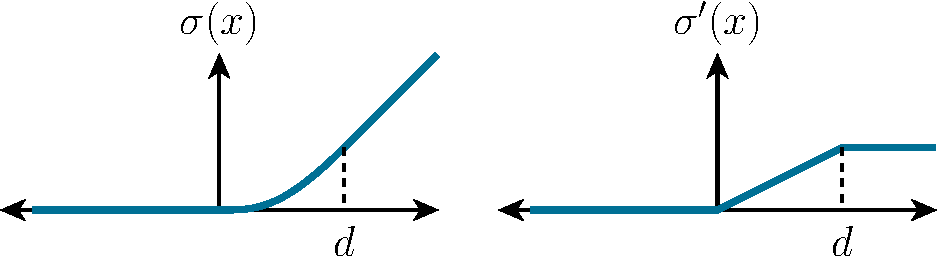
\includegraphics[width=.66\textwidth]{LSDDM/figures/rehu.pdf}
    \caption{Rectified Huber Unit (ReHU), necessary for continuously differentiable Lyapunov functions. }
    \label{fig:rehu}
\end{figure}
% \end{comment}

\paragraph{Continuously differentiable.}  Although not always required, several of the conditions for Lyapunov stability are simplified if $V$ is continuously differentiable. ReLU is discontinuous around 0, and the soft-plus smoothed ReLU is not zero at the origin. We use a smoothed version with quadratic knee in $[0, d]$, called the Rectified Huber Unit (ReHU):
\begin{align}
	\sigma(x) = \begin{cases} 0                   & \mbox {if } x \leq 0 \\
              \nicefrac{x^2}{2d}  & \mbox{if } 0 < x < d \\
              x - \nicefrac{d}{2} & \mbox{otherwise}\end{cases}.
\end{align}
An illustration of this activation is shown in Figure \ref{fig:rehu}.

\paragraph{[Optional] Warped input space. }  Our construction so far guarantees that the Lyapunov function has no local optima by making it convex. This is sufficient but not necessary, and it may even impose too strict a constraint on the learned dynamics. We can relax this function by allowing the input to the ICNN to be warped by any continuously differentiable invertible function $F : \mathbb{R}^n \times \mathbb{R}^n$. i.e., using
\begin{align}
	V(x) = \sigma_{k+1}(g(F(x)) - g(F(0))) + \epsilon \|x\|_2^2.
	\label{eq:V_definition2}
\end{align}
as the Lyapunov function.  Invertibility ensures that the level sets of $V$, which are convex, map to contiguous regions of the composite function $g \circ F$. This allows the resultant Lyapunov function to be non-convex without having any optima other than the global.

With these conditions in place, we have the following result.
\begin{theorem}
	The dynamics defined by
	\begin{align}
		\dot{x} = f(x)
	\end{align}
	are globally exponentially stable to the equilibrium point $x=0$. Where $f$ is from Eqn.~\eqref{eq:dynamics} and $V$ is from Eqn.~\eqref{eq:V_definition} or Eqn.~\eqref{eq:V_definition2}, and $\hat{f}$ and $V$ functions have finite, bounded weights.
\end{theorem}
\begin{proof}
	The proof is straightforward, and relies on the properties of the networks created above.  First, note that by our definitions we have, for some $M$,
	\begin{align}
		\epsilon \|x\|^2_2 \leq V(x) \leq M \|x\|_2^2
	\end{align}
	where the lower bound follows from Eqn.~\ref{eq:V_definition} and the fact that $g$ is positive. The upper bound follows from the fact that the ReHU activation is linear for large $x$ and quadratic around 0.  This fact in turn implies that $V(x)$ behaves linearly as $\|x\|\rightarrow \infty$, and is quadratic around the origin, so can be upper bounded by some quadratic $M \|x\|_2^2$.

	The fact the $V$ is continuously differentiable means that $\nabla V(x)$ (in $f$) is defined everywhere, bounds on $\|\nabla V(x)\|_2^2$ for all $x$ follows from the the Lipschitz property of $V$, the fact that $0 \leq \sigma'(x) \leq 1$, and the $\epsilon \|x\|_2^2$ term
	\begin{align}
		\epsilon \|x\|_2 \leq  \|\nabla V(x)\|_2 \leq \sum_{i=1}^k \prod_{j=i}^k \|U_j\|_2 \|W_i\|_2
	\end{align}
	where $\|\cdot\|_2$ denotes the operator norm when applied to a matrix.  This implies that the dynamics are defined and bounded everywhere owing to the choice of function $\hat{f}$.

	Now, consider some initial state $x(0)$.  The definition of $f$ implies that
	\begin{align}
		\frac{d}{dt} V(x(t))  & = \nabla V(x)^T \frac{d}{dt} x(t) = \nabla V(x)^T f(x) \leq -\alpha V(x(t)).
		\intertext{Integrating this equation gives the bound}
		V(x(t))               & \leq V(x(0))e^{-\alpha t}
		\intertext{and applying the lower and upper bounds gives}
		\epsilon \|x(t)\|_2^2 & \leq M \|x(0)\|_2^2 e^{-\alpha t}
		\; \Longrightarrow \; \|x(t)\|_2 \leq \frac{M}{\epsilon} \|x(0)\|_2 e^{-\alpha t/2}
	\end{align}
	as required for global exponential convergence.
\end{proof}




\section{Empirical results}

We illustrate our technique on several example problems, first highlighting the (inherent) stability of the method for random networks, demonstrating learning on simple $n$-link pendulum dynamics, and finally learning high-dimensional stable latent space dynamics for dynamic video textures via a VAE model.

\subsection{Random networks}


\begin{figure}
    \centering
    \begin{tikzpicture}
        \begin{groupplot}[
                group style={
                        group name=my plots,
                        group size=4 by 1,
                        ylabels at=edge left,
                        yticklabels at=edge left,
                        horizontal sep=12pt
                    },
                axis on top,% ----
                width=1.33in,
                height=1.33in,
                scale only axis,
                enlargelimits=false,
                xmin=-2,
                xmax=2,
                ymin=-2,
                ymax=2,
            ]

            \nextgroupplot[title={Nominal $\hat f$}]
            \addplot[] graphics[xmin=-2,ymin=-2,xmax=2.2,ymax=2.2] {LSDDM/figures/random/fhat_dynamics.eps};
            \nextgroupplot[title={Lyapunov Function $V$}]
            \addplot[] graphics[xmin=-2,ymin=-2,xmax=2,ymax=2] {LSDDM/figures/random/V_lyap.eps};
            \nextgroupplot[axis equal image, axis lines=none, xtick=\empty, ytick=\empty]
            \addplotgraphicsnatural [xmin=-2, xmax=2, ymin=-2, ymax=2] {LSDDM/figures/pendulum/nn-lyapunov-cmap.eps};
            \nextgroupplot[title={Stable $f$}]
            \addplot[] graphics[xmin=-2,ymin=-2,xmax=2.2,ymax=2.2] {LSDDM/figures/random/f_dynamics.eps};
        \end{groupplot}
    \end{tikzpicture}
    \caption{(left) Nominal dynamics $\hat{f}$ for random network; (center) Convex positive definite Lyapunov function generated by random ICNN with constraints from Section \ref{sec:lyapunov_properties}; (right) Resulting stable dynamics $f$.}
    \label{fig:nominal_dynamics}
\end{figure}


Although we mention this only briefly, it is interesting to visualize the dynamics created by random networks according to our process, i.e., before any training at all. Because the dynamics models are inherently stable, these random networks lead to stable dynamics with interesting behaviors, illustrated in Figure \ref{fig:nominal_dynamics}.  Specifically, we let $\hat{f}$ be defined by a fully connected network and $V$ be an ICNN. Both networks have two hidden layers with 100 nodes each, and are initialized by the Kaiming uniform initialization \citep{he2015delving}). The $U$ weights in the ICNN are further subject to a softplus unit to make them positive.

\subsection[n-link pendulum]{$n$-link pendulum}

Next we look at the ability of our approach to model a physically-based dynamical system, specifically the $n$-link pendulum.  A damped, rigid $n$-link pendulum's state $x$ can be described by the angular position $\theta_i$ and angular velocity $\theta_i$ of each link $i$.  As before $\hat f$ and the Lyapunov function $V$ have two hidden layers of 100 nodes, with properties described in Section~\ref{sec:lyapunov_properties}. Models are trained with pairs of data $(x, \dot x)$ produced by the symbolic algebra solver \texttt{sympy}, using simulation code adapted from \cite{vanderplas_2017}.


\begin{figure}
    \centering
    \begin{tikzpicture}
        \begin{groupplot}[
                group style={
                        group name=my plots,
                        group size=4 by 1,
                        ylabels at=edge left,
                        yticklabels at=edge left,
                        horizontal sep=18pt
                    },
                axis on top,% ----
                width=1.33in,
                height=1.33in,
                scale only axis,
                enlargelimits=false,
                xmin=-2,
                xmax=2,
                ymin=-2,
                ymax=2,
            ]

            \nextgroupplot[title={Simulated}]
            \addplot[] graphics[xmin=-2,ymin=-2,xmax=2,ymax=2] {LSDDM/figures/pendulum/true-stream.eps};
            \nextgroupplot[title={Learned $f$}]
            \addplot[] graphics[xmin=-2,ymin=-2,xmax=2,ymax=2] {LSDDM/figures/pendulum/nn-stream.eps};
            \nextgroupplot[title={Learned $V$}]
            \addplot[] graphics[xmin=-2,ymin=-2,xmax=2,ymax=2] {LSDDM/figures/pendulum/nn-lyapunov.eps};
            \nextgroupplot[axis equal image, axis lines=none, xtick=\empty, ytick=\empty]
            \addplotgraphicsnatural [xmin=-2, xmax=2, ymin=-2, ymax=2] {LSDDM/figures/pendulum/nn-lyapunov-cmap.eps};
        \end{groupplot}
    \end{tikzpicture}
    \caption{Dynamics of a simple damped pendulum. From left to right: the dynamics as simulated from first principles, the dynamics model $f$ learned by our method, and the Lyapunov function $V$ learned by our method (under which $f$ is non-expansive).}
    \label{fig:pendulum_experiment}
\end{figure}{}


In Figure~\ref{fig:pendulum_experiment}, we compare the simulated dynamics with the learned dynamics in the case of a simple damped pendulum (i.e. with $n=1$), showing both the vector field and a single simulated trajectory, and draw a contour plot of the learned Lyapunov function. As seen, the system is able to learn dynamics that can accurately predict motion of the system even over long time periods.

\pgfplotstableread{LSDDM/figures/pendulum_results/nlinkerror_simple.dat}{\nlinkerrorsimple}
\pgfplotstableread{LSDDM/figures/pendulum_results/nlinkerror_rehu.dat}{\nlinkerrorrehu}
\pgfplotstableread{LSDDM/figures/pendulum_results/8_simple.dat}{\pendressimple}
\pgfplotstableread{LSDDM/figures/pendulum_results/8_REHU_0.005.dat}{\pendressrehu}
\pgfplotstableread{LSDDM/figures/pendulum_results/8_lstm.dat}{\pendresslstm}

\begin{figure}
    \begin{center}
        \begin{tikzpicture}
            \begin{groupplot}[
                    group style={
                            group name=my plots,
                            group size=2 by 1,
                            ylabels at=edge left,
                            yticklabels at=edge left,
                            horizontal sep=12pt
                        },
                    axis on top,% ----
                    height=1.2in,
                    width=2.35in,
                    scale only axis,
                    enlargelimits=false,
                    ymode=log
                ]

                \nextgroupplot[title={\shortstack{Error at each time\\ for 8-link pendulums}},
                    axis on top,% ----
                    scale only axis,
                    enlargelimits=false,
                    xmin=0, xmax=1000, ymin=100, ymax=100000,
                    ylabel near ticks,
                    legend pos=north west,
                    xlabel={Timestamp},
                    ylabel={Error}]

                \addplot+[]
                table [x={t}, y={loss}] {\pendressimple};
                \addplot+[]
                table [x={t}, y={loss}] {\pendressrehu};
                \legend{Simple,Stable}

                \nextgroupplot[title={\shortstack{Average error over 999 timesteps\\ for $n$-link pendulums}},
                    xmin=0.5, xmax=8.5,
                    ymin=10000, ymax=100000000,
                    xlabel={Number of links $n$}, xtick=data]
                \addplot+[] table [x={n}, y={loss}] {\nlinkerrorsimple};
                \addplot+[] table [x={n}, y={loss}] {\nlinkerrorrehu};

            \end{groupplot}
        \end{tikzpicture}
    \end{center}

    \caption{Error in predicting $
            \theta, \dot \theta$ in 8-link pendulum at each timestep (left); and average error over 999 timesteps as the number of links in the pendulum increases (right).}
    \label{fig:pendulum_results}
\end{figure}


We also evaluate the learned dynamics quantitatively varying $n$ and the time horizon of simulation. Figure~\ref{fig:pendulum_results} presents the total error over time for the 8-link pendulum, and the average cumulative error over 1000 time steps for different values of $n$.  While both the simple and our stable models show increasing mean error at the start of the trajectory, our model is able to capture the contraction in the physical system (implied by conservation of energy) and in fact exhibits decreasing error towards the end of the simulation (the true and simulated dynamics are both stable). In comparison, the error in the simple model increases.

\subsection{Video Texture Generation}

Finally, We apply our technique to stable video texture generation, using a Variational Autoencoder (VAE) \citep{kingma2013auto} to learn an encoding for images, and our stable network to learn a dynamics model in encoding-space.  Given a sequence of frames $(y_0, y_1, \ldots)$, we feed the network the frame at time $t$
and train it to reconstruct the frames at time $t$ and $t+1$.  Specifically, we consider a VAE defined by the encoder $e : \mathcal{Y} \rightarrow \mathbb{R}^{2n}$ giving mean and variance $\mu, \log \sigma^2_t = e(y_t)$, latent state $z_t \in \mathbb{R}^n \sim \mathcal{N}(\mu_t, \sigma_t^2)$, and decoder $d: \mathbb{R}^n \rightarrow \mathcal{Y}$, $y_t \approx d(z_t)$.  We train the network to minimize both the standard VAE loss (reconstruction error plus a KL divergence term), but \emph{also} minimize the reconstruction loss of a next predicted state. We model the evolution of the latent dynamics at $z_{t+1} \approx f(z_t)$, or more precisely $y_{t+1} \approx d(f(z_t))$.  In other words, as illustrated in Figure~\ref{fig:vae_training}, we train the full system to minimize
\begin{align}
	\minimize_{e,d,\hat{f},V} \sum_{t=1}^{T-1} \biggl ( \mathsf{KL}(\mathcal{N}(\mu_t,\sigma_t^2 I\|\mathcal{N}(0,I)) + \mathbf{E}_z \bigl [ \|d(z_t) - y_t\|_2^2 + \| d(f(z_t)) - y_{t+1}\|_2^2 \bigr ] \biggr )
\end{align}



\begin{figure}
    \begin{tikzpicture}
        \begin{axis}[
                axis on top,% ----
                scale only axis,
                enlargelimits=false,
                xmin=0, ymin=0,
                xmax=527.577, ymax=134.747,
                width=5.5in,
                height=1.404in,
                yticklabels={,,},
                xticklabels={,,},
                axis line style={draw=none},
                tick style={draw=none}]
            \addplot[] graphics[xmin=0, ymin=0, xmax=527.577, ymax=134.747] {LSDDM/figures/vidtex-2/model-training-blank.png};
            \node (A) [anchor=north] at (axis cs:40,74){$e(y_t)$};
            \node (D) [anchor=south west] at (axis cs:66,102){$\mu_t$};
            \node (E) [anchor=north west] at (axis cs:66,82){$\log\sigma_t$};
            \node (H) [anchor=south west] at (axis cs:160,64){\small{$\hat f(z_t)$}};
            \node (H) [anchor=south west] at (axis cs:160,28){\small{$V(z_t)$}};
            \node (F) [anchor=south] at (axis cs:196,92){$z_t \in \mathcal{N}(\mu_t,\sigma_t^2)$};
            \node (J) [anchor=south] at (axis cs:286,35){\footnotesize{$z_{t+1} \gets z_t + f(z_t)$}};
            \node (B) [anchor=north east] at (axis cs:392,72){\footnotesize{$d(z_t)$}};
            \node (B) [anchor=north east] at (axis cs:392,20){\footnotesize{$d(z_{t+1})$}};
            \node (I) [anchor=west] at (axis cs:380,118){{KL}($\mathcal{N}(\mu_t,\sigma_t^2)\| \mathcal{N}(0,I))$};
            \node (K) [anchor=west] at (axis cs:396,82){$\|d(z_t) - y_{t}\|_2^2$};
            \node (K) [anchor=west] at (axis cs:396,28){$\|d(z_{t+1}) - y_{t+1}\|_2^2$};
        \end{axis}
    \end{tikzpicture}
    \caption{Structure of our video texture generation network. The encoder $e$ and decoder $d$ form a Variational Autoencoder, and the stable dynamics model $f$ is trained together with the decoder to predict the next frame in the video texture.}
    \label{fig:vae_training}
\end{figure}

\setlength{\tabcolsep}{2pt}
\newcommand{\sampletbl}[2]{
    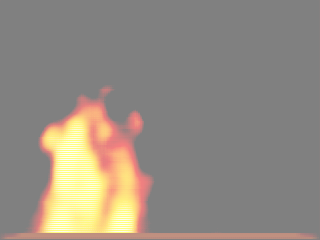
\includegraphics[width=0.4in]{LSDDM/figures/results/#1-#2/fr_00000.png} &
    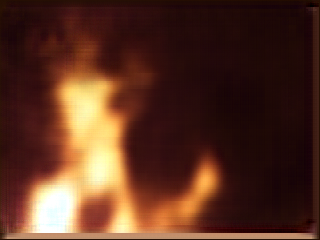
\includegraphics[width=0.4in]{LSDDM/figures/results/#1-#2/fr_00010.png} &
    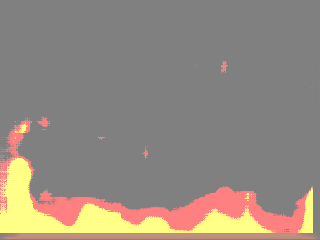
\includegraphics[width=0.4in]{LSDDM/figures/results/#1-#2/fr_00020.png} &
    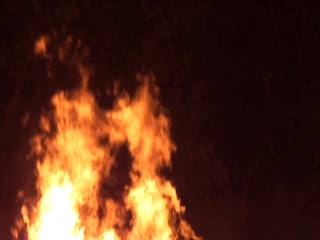
\includegraphics[width=0.4in]{LSDDM/figures/results/#1-#2/fr_00030.png} &
    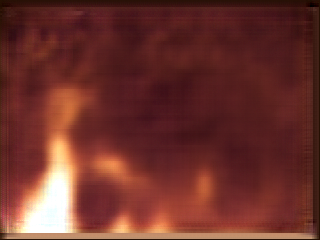
\includegraphics[width=0.4in]{LSDDM/figures/results/#1-#2/fr_00040.png} &
    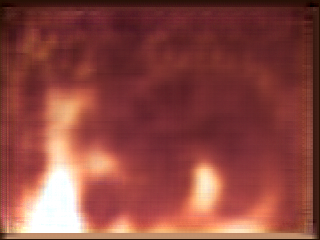
\includegraphics[width=0.4in]{LSDDM/figures/results/#1-#2/fr_00050.png}  &
    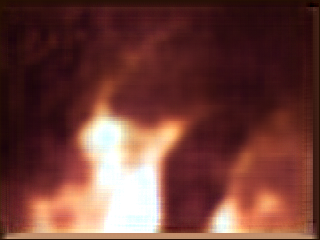
\includegraphics[width=0.4in]{LSDDM/figures/results/#1-#2/fr_00100.png} &
    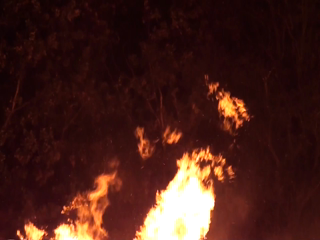
\includegraphics[width=0.4in]{LSDDM/figures/results/#1-#2/fr_00150.png} &
    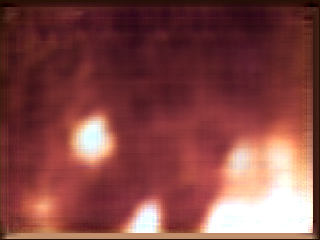
\includegraphics[width=0.4in]{LSDDM/figures/results/#1-#2/fr_00200.png} &
    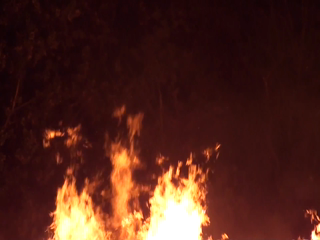
\includegraphics[width=0.4in]{LSDDM/figures/results/#1-#2/fr_00250.png}
}
\begin{figure}
    \centering
    \begin{tikzpicture}
        \begin{groupplot}[
                group style={
                        group name=my plots,
                        group size=5 by 1,
                        horizontal sep=12pt
                    },
                axis on top,% ----
                width=1.in,
                height=1.in,
                scale only axis,
                enlargelimits=false,
                xmin=0,
                xmax=1,
                ymin=0,
                ymax=1,
                axis x line*=bottom, axis y line*=left,
            ]

            \nextgroupplot[title={Stable Model Run 1},
                ytick={.1, 1},
                yticklabels={-2,18},
                xtick={.15, 1},
                xticklabels={$-10$,15}]
            \addplot[
                yticklabels={,,},
                xticklabels={,,}] graphics[xmin=-0.17,ymin=-0.17,xmax=1.17,ymax=1.17] {LSDDM/figures/results/bonfire-exp27r-1e-5-1231132/trajmodel.png};

            \nextgroupplot[title={Stable Model Run 2},
                ytick={.1, 1},
                yticklabels={0,$20$},
                xtick={.15, 1},
                xticklabels={$0$,25}]
            \addplot[] graphics[xmin=-0.17,ymin=-0.17,xmax=1.17,ymax=1.17] {LSDDM/figures/results/bonfire-exp27r-1e-5-1238886/trajmodel.png};

            \nextgroupplot[title={Stable Model Run 3},
                ytick={.1, 1},
                yticklabels={-10,8},
                xtick={.1, .8},
                xticklabels={-5,15}]
            ]
            \addplot[] graphics[xmin=-0.17,ymin=-0.17,xmax=1.17,ymax=1.17] {LSDDM/figures/results/bonfire-exp27r-1e-5-main/trajmodel.png};

            \nextgroupplot[title={Naive Model},
                ytick={.1, 1},
                yticklabels={0,},
                xtick={.1, 1},
                xticklabels={$-2 \times 10^{30}$,0},
                extra y tick labels={$1.2 \times 10^{30}$},
                extra y ticks={1.0},
                extra y tick style={y tick label style={right, xshift=0.25em}},]
            \addplot[] graphics[xmin=-0.17,ymin=-0.17,xmax=1.17,ymax=1.17] {LSDDM/figures/results/bonfire-bad2/trajmodel.png};

            \nextgroupplot[
                ytick={0,1},
                yticklabels={0,300},
                ylabel={steps},
                width=.05in,
                axis line style={draw=none}, tick style={draw=none}, xticklabel=\empty, every axis y label/.style={at={(current axis.west)},rotate=90,yshift=-3mm,xshift=1mm},
                y tick label style={right, xshift=0.25em}]

            \addplot[] graphics[xmin=0,ymin=0,xmax=1,ymax=1] {LSDDM/figures/viridis.png};

        \end{groupplot}
    \end{tikzpicture}
    \begin{tabular}{r|cccccc|cccc}
        Stable & \multicolumn{10}{c}{Frame Number}                                                                                             \\
        Model  & $0$                                      & ${10}$ & ${20}$ & ${30}$ & ${40}$ & ${50}$ & ${100}$ & ${150}$ & ${200}$ & ${250}$ \\
        Run 1  & \sampletbl{bonfire}{exp27r-1e-5-main}                                                                                         \\
        Run 2  & \sampletbl{bonfire}{exp27r-1e-5-1231132}                                                                                      \\
        Run 3  & \sampletbl{bonfire}{exp27r-1e-5-1238886}                                                                                      \\
        \shortstack{Naive                                                                                                                      \\Model} &
        \sampletbl{bonfire}{bad2}
        % \\ \shortstack{Sample\\Video} &    \sampletbl{bonfire}{sample}
    \end{tabular}

    \caption{Samples generated by our stable video texture networks, with associated trajectories above. The true latent space is 320-dimensional; we project the trajectories onto a two-dimensional plane for display. For comparison, we present the video texture generated using an unconstrained neural network in place of our stable dynamics model.}
    \label{fig:vae_results}
\end{figure}


We train the model on pairs of successive frames sampled from videos. To generate video textures, we seed the dynamics model with the encoding of a single frame and numerically integrate the dynamics model to obtain a trajectory. The VAE decoder converts each step of the trajectory into a frame. In Figure~\ref{fig:vae_results}, we present sample stable trajectories and frames produced by our network. For comparison, we also include an example trajectory and resulting frames when the dynamics are modelled without the stability constraint (i.e. letting $f$ in the above loss be a generic neural network).  For the naive model, the dynamics quickly diverge and produce a static image, whereas for our approach, we are able to generate different (stable) trajectories that keep generating realistic images over long time horizons.

\section{Conclusion}

We proposed a method for learning stable non-linear dynamical systems defined by neural network architectures. The approach jointly learns a convex positive definite Lyapunov function along with dynamics constrained to be stable according to these dynamics everywhere in the state space.  We show that these models can be integrated into other deep architectures such as VAEs, and learn complex latent space dynamics is a fully end-to-end manner.  Although we have focused here on the autonomous (uncontrolled) setting, the method opens several directions for future work, such as integration into dynamical systems for control or reinforcement learning settings.  Have stable systems as a ``primitive'' can be useful in a large number of contexts, and combining these stable systems with the representational power of deep networks offers a powerful tool in modeling and controlling dynamical systems.


\section{Adaptation to Stable Control and RL }

After the successes of our stable dynamics model, we attempted to extend it to also learn stable policies and value functions. The intuitive extension to this is to replace the dynamics model $\hat f$ with fixed (known) dynamics $\tilde f$ and a learnable policy network $\pi$. That is, we train to minimize:
\begin{align}
  \mathsf{ReLU}\bigl(\nabla V(x)^T \tilde{f}(x, \pi) + \alpha V (x) \bigr)
\end{align}
given traces from simulated dynamics. We also transformed the dynamics so that the goal state was positioned at the origin, choosing suitable transformations for the dynamics and Lyapunov functions. As required by the approach, we attempted to train it from trajectory samples to minimize the error over one step.

We were able to successfully learn stabilizing controllers for toy examples such as a simple damped pendulum and for the cartpole problem. Unfortunately, we were not able to learn a swing-up controller for either environment, or any type of controller for an Acrobot\footnote{A two-link pendulum with a single actuator in the middle joint. } or more complex locomotion tasks. We observed that the training would consistently fail in the same way: the nominal dynamics function would diverge to the point of uselessness, followed by the learned Lyapunov function collapsing to a trivial function.

This persisted despite any amount of regularization, hyperparameter tuning, and even across a variety of environments. Contemporary efforts in the literature were similarly unable to scale this approach to locomotion tasks. The consistent failure of this method suggested that an underlying principle was being violated, and that regularization was not able to address that. We eventually investigated how the difference in distributions between the data used to train the purportedly stable controller and the policy the controller was attempting to learn, which led us to the work in the next chapter.



%%%%%%%%%%%%%%%%%%%%%%%%%%%%%%%%%%%%
\chapter[The Pitfalls of Regularization in Off-Policy TD]{The Pitfalls of Regularization in Off-Policy Temporal Difference Learning}
\chaptermark{Regularization in Off-Policy TD}

Temporal Difference (TD) learning is ubiquitous in reinforcement learning, where it is often combined with off-policy sampling and function approximation.  Unfortunately learning with this combination (known as the \emph{deadly triad}), exhibits instability and unbounded error.  To account for this, modern RL methods often implicitly (or sometimes explicitly) assume that regularization is sufficient to mitigate the problem in practice; indeed, the standard deadly triad examples from the literature can be ``fixed'' via proper regularization. In this paper, we introduce a series of new counterexamples to show that the instability and unbounded error of TD methods is \emph{not} solved by regularization. We demonstrate that, in the off-policy setting with linear function approximation, TD methods can fail to learn a non-trivial value function under \emph{any} amount of regularization; we further show that regularization can induce divergence under common conditions; and we show that one of the most promising methods to mitigate this divergence (Emphatic TD algorithms) may also diverge under regularization. We further demonstrate such divergence when using neural networks as function approximators.  Thus, we argue that regularization in TD methods needs to be reconsidered, given that it is insufficient to prevent divergence and may itself introduce instability. There needs to be much more care in the application of regularization to RL methods.

\emph{From ``The Pitfalls of Regularization in Off-Policy TD Learning'' by \citeauthor{manek2022pitfalls} (\citeyear{manek2022pitfalls})}

\clearpage

%%%%%%%%%%%%%%%%%%%%%%%%%%%%%%%%%%%%%%%%%%%%%%%%%%%%%%%%%%%%
\section{Introduction}
Temporal Difference (TD) learning is a method for learning expected future-discounted quantities from Markov processes, using transition samples to iteratively improve estimates. This is most commonly used to estimate expected future-discounted rewards (the \emph{value function}) in Reinforcement Learning (RL). Advances in RL allow us to use powerful function approximators, and also to use sampling strategies other than naively following the Markov process (MP). When TD, function approximation, and off-policy training are all combined, learned functions exhibit severe instability and divergence, as classically observed by \citet{baird1993counterexample,tsitsiklis1996analysis}. This combination is known in the literature as the \emph{deadly triad}~\cite[pg.~264]{sutton2020reinforcement}, and while many contemporary variants of TD are designed to converge despite the instability, the quality of the solution at convergence may be arbitrarily poor.

A common technique to avoid unbounded error is $\ell_2$ \emph{regularization}~\cite{tikhonov1943stability}, i.e.\ penalizing the squared norm of the weights in addition to the TD error.  This is generally understood to bound the worst-case error in exchange for biasing the model and potentially increasing the error everywhere else.  When used on three common examples of the deadly triad~\cite[pg.260]{kolter2011fixed,baird1993counterexample,sutton2020reinforcement}, regularization appears to mitigate the worst aspects of the divergence in practice.  Consequently, it has become an essential assumption made by many RL algorithms~\cite{diddigi2019convergent,mahadevan2014proximal,sutton2009fast,yu2017convergence,zhang2020provably,zhang2021breaking,kumar2022dr} and is seen as routine and innocuous.

We argue that this perspective on regularization in off-policy TD is fundamentally mistaken.  While regularization is indeed reasonably well-behaved and innocuous in classic fully-supervised contexts, the use of bootstrapping in TD means that even small amounts of model bias induced by regularization can cause divergence.  This is an oft-ignored phenomenon in the literature, and so we introduce a series of new counterexamples (summarized in Table~\ref{tab:summarytheorems}) to show how regularization can have counterintuitive and destructive effects in TD.  We show that vacuous solutions and training instability are \emph{not} solved by the use of regularization; that applying regularization can sometimes induce divergence and increase worst-case error; and that Emphatic TD algorithms---which are the most promising solution to this divergence---can themselves diverge when regularized. We finally also illustrate misbehaving regularization in the context of neural network value function approximation, demonstrating the general pitfalls of regularization possible in RL algorithms.  Regularization needs to be treated cautiously in the context of RL, as it behaves differently than in supervised settings.

Our counterexamples demonstrate these core ideas:

\paragraph{TD learning off-policy can be unstable and/or have unbounded error even when it converges.}
Following well-established methods we show there is some off-policy distribution under which TD with linear value function approximation diverges \emph{and} learns a model with unbounded error (even if it were able to converge to the TD fixed point). This concisely demonstrates key features of the training error: the error is small when the distribution is close to on-policy, but the error diverges around specific off-policy distributions.  The intuition behind this, explained in Section~\ref{sec:introduce_example}, is that the off-policy\footnote{We consider a sampling distribution to be \emph{on-policy} if it follows the stationary distribution of the MP;  we do not explicitly consider a separate policy in this paper. } TD update involves a projection operation that depends on the sampling distribution and can be arbitrarily far away from the true value.  This basic fact has already been established by past work~\cite{baird1993counterexample,kolter2011fixed}, but our example is based upon a particular simple three-state MP, drawn in Figure~\ref{fig:mdp_illustration}.

\paragraph{Regularization cannot always mitigate off-policy training error. }
We next introduce regularization into our setting, and show how it changes the relationship between training error and off-policy training. As explained in Section~\ref{sec:introduce_ab}, we penalize the $\ell_2$-norm of learned (linear) weights with some coefficient $\eta$; as $\eta$ increases, the learned weights approach zero.  However, in \textbf{Example~\ref{ex:withrr}}, we show that there exists an off-policy distribution such that for any $\eta \geq 0 < \infty$, the regularized TD fixed point attains strictly higher approximation error than the zero solution (i.e., the infinitely regularized point).  We call such examples \emph{vacuous}. In other words, \emph{vacuous value functions never do better than guessing zero for all states, for any amount of regularization}.

We further analyze this vacuous example in the context of the algorithm in \citep{zhang2021breaking}. In this work, the authors assume the use of regularization to derive bounds on the learned error under off-policy sampling. Although these bounds are technically correct in the case of our counterexample, they are very loose, at about $2000$ times the threshold of vacuity.  This highlights the challenge of formally relying on regularization to bound model error.

\paragraph{Small amounts of regularization can cause model divergence or large errors. }
There is a general implicit assumption in much ML literature that regularization monotonically shrinks learned weights. This intuition comes from classic fully-supervised machine learning where it typically holds. But because TD bootstraps value estimates (i.e.\ learns values using its own output), it is possible for small amounts of bias to be arbitrarily magnified. We dub this phenomenon ``small-eta error'' and illustrate it in \textbf{Example~\ref{ex:badeta}}. We relate this to the presence of negative eigenvalues in an intermediate step of the solution and % show how this causes models that are otherwise well-behaved to diverge around specific values of $\eta$.  
show that, in some settings, the error of the TD solution may be relatively small when applied with no regularization but adding regularization causes the model to have worse error than the zero solution.

One common solution to this problem is to lower-bound $\eta$ to guarantee that regularization behaves monotonically. However, we further show that such a lower bound may occur after the point of vacuity: a model that is not vacuous becomes vacuous for any regularization parameter above this lower bound. We also show that it is not always possible to select a single $\eta$ \emph{a priori}, with examples of mutually-incompatible off-policy distributions where there is no $\eta$ that achieves better than vacuous or nearly-vacuous results at different distributions.


\paragraph{Emphatic-TD-based algorithms are vulnerable to instability from regularization.  }
Emphatic-TD~\cite{sutton2016emphatic} fundamentally solves the problem of training off-policy by resampling TD updates so they appear to be on-policy.  This technique requires an emphasis model that decides how to scale each TD update, and learning this has been the key challenge preventing widespread adoption of Emphatic-TD.  A recent paper~\cite{zhang2020provably} proposed learning this emphasis model using ``reversed'' TD while simultaneously learning the value model using regular TD.  The resultant algorithm is called COF-PAC, and employs regularization to ensure that the two TD models eventually converge.

We show that regularization, while necessary, can be harmful for such models in \textbf{Example~\ref{ex:emph}}. Specifically, we construct a model that converges to the correct solution without regularization but to an arbitrarily poor solution when regularized. The intuition behind this is that regularizing the emphasis model changes the effective distribution of the TD updates to the value model, which can cause the value model to have arbitrarily large error. We complete the example by showing that regularizing the value function separately does not restore performance.

\paragraph{Regularization can cause model divergence in neural networks. }
So far most analysis of the deadly triad in the literature focuses on the linear case. We extend our example to a nine-state Markov chain (shown in Figure~\ref{fig:mdp9_illustration}), and show how the previously identified problems persist into the neural network case in \textbf{Example~\ref{ex:neuralnetwork}}. We show two key similarities: first, models trained at certain off-policy distributions may be vacuous. Second, small amounts of regularization counterintuitively \emph{increase} error. This illustrates Example~\ref{ex:badeta} in the NN case.

\begin{table}
	\centering
	\begin{tabular}{p{0.15\textwidth} p{0.85\textwidth}}
		\toprule\toprule
		%    Theorem & Description \\
		%    \midrule
		\\  \textbf{Example~\ref{ex:withrr}} & There exist off-policy distributions under which TD learns a \emph{vacuous} model (one which---despite any amount of regularization---never does better than guessing zeros).
		\\  \textbf{Example~\ref{ex:badeta}} & Small values of the regularization parameter $\eta$ can make TD diverge in models that otherwise converge. This is an unavoidable effect of bootstrapping in TD, and setting a lower-bound to exclude this may render models vacuous.
		\\  \textbf{Example~\ref{ex:emph}} & Emphatic-TD-inspired algorithms are a promising way to reweigh samples and mitigate the effects of training off-policy. But if this reweighing is learned using TD, then using regularization can bias the emphasis model and cause the value model itself to diverge.
		\\  \textbf{Example~\ref{ex:neuralnetwork}} & Training instability and increased error due to the deadly triad also occur when neural networks are used. We construct an empirical example and draw qualitative comparisons.
		\\ \bottomrule \bottomrule
	\end{tabular}
	\vspace{7pt}
	\caption{Summary of theorems. }\label{tab:summarytheorems}
\end{table}

\begin{figure}
	\centering
\begin{subfigure}[b]{0.49\textwidth}
  \centering
  \begin{tikzpicture}[->,shorten >=1pt, node distance={15mm}, main/.style = {draw, circle}] 
    \node[main] (3) {$s_3$}; 
    \node[main] (1) [below left of=3] {$s_1$}; 
    \node[main] (2) [below right of=3]{$s_2$}; 

    \path
    (1) edge[bend left=-30] node[above] {\sfrac 1 4} (2)
        edge[bend right=-10] node[below right] {\sfrac 1 2} (3)
        edge[loop left] node[left] {\sfrac 1 4} (1);

    \path
    (2) edge[bend left=40] node[below] {\sfrac 1 4} (1)
        edge[bend left=-10] node[below left] {\sfrac 1 2} (3)
        edge[loop right] node[right] {\sfrac 1 4} (2);

    \path
    (3) edge[bend left=20] node[above right] {\sfrac 1 4} (2)
        edge[bend right=20] node[above left] {\sfrac 1 4} (1)
        edge[loop above,out=80,in=110,looseness=5] node[left=2mm,pos=0.2] {\sfrac 1 2} (3);

  \end{tikzpicture}
  \caption{Three-state MP. }
  \label{fig:mdp_illustration}
\end{subfigure}
\begin{subfigure}[b]{0.49\textwidth}
    \begin{align}
        \frac{1}{4}\begin{bmatrix}
            1 & 1 & 2 \\ 1 & 1 & 2 \\ 1 & 1 & 2
        \end{bmatrix}
    \end{align}
    \caption{Three-state MP. }
    \label{fig:mdp_transition}
\end{subfigure}

	\caption{Our three-state counterexample Markov Process. We use this to illustrate how TD models can fail despite common mitigating strategies with linear function approximation. }\label{fig:mdp}
\end{figure}

%%%%%%%%%%%%%%%%%%%%%%%%%%%%%%%%%%%%%%%%%%%%%%%%%%%%%%%%%%%%
\section{Preliminaries and Notation}

Consider the $n$-state Markov chain $(\mathcal S, P, R, \gamma)$, with state space $\mathcal S$, state-dependent reward $R : \mathcal S \to \mathbb R$, and discount factor $\gamma \in [0, 1]$. $P \in \mathbb R^{n\times n}$ is the transition matrix, with $P_{ij}$ encoding the probability of moving from state $i$ to $j$. We wish to estimate the value function $V : \mathcal S \to R$, defined as the expected discounted future reward of being in each state: $V(s) \dot = \textbf E\left[\left.\sum_{t=0}^\infty \gamma^t R(s_t) \right| s_0 = s \right]$. A key property is that it follows the Bellman equation:
\begin{align}
	V      & = R + \gamma PV
	\intertext{Using linear function approximation to learn $V$, we assume a matrix of feature-vectors $\Phi\in\mathbb R^{n\times k}$ that is fixed, and a vector of parameters $w\in \mathbb R^k$ that is learned. The Bellman equation is then:}
	\Phi w & = R + \gamma\,P\,\Phi w
	\intertext{When $w$ is learned with TD, this equation is only valid if the TD updates are \emph{on-policy} (that is, they are distributed according to the steady-state probability of visiting each state, written as $\pi \in \mathbb R^n$). In the general case, where TD updates follow a (possibly) different distribution $\mu\in \mathbb R^n_0$, the TD solution is a fixed point of the Bellman operator followed by a projection~\cite{kolter2011fixed}:}
	\Phi w & = \Pi_\mu \left( R + \gamma P \Phi w \right)
	\intertext{where the matrix $\Pi_\mu = \Phi {(\Phi^\top D \Phi)}^{-1} \Phi^\top D$ projects the Bellman backup onto the column-space of $\Phi$, reweighed by the diagonal matrix $D = \text{diag}(\mu)$. This yields the closed-form solution:}
	w      & = A^{-1} \vec b
\end{align}
Where $A = \Phi^\top D (I - \gamma P) \Phi$ and $\vec b = \Phi^\top D R$. When this solution is subject to $\ell_2$ regularization, some non-negative $\eta$ is added to ensure the matrix being inverted is positive definite:
\begin{align}
	w^*(\eta) & = {(A + \eta I)}^{-1} \vec b \label{eqn:wstar}
\end{align}
As will be important later, we note that as $\eta$ increases it drives $w^*(\eta)$ towards zero.\label{sec:introduce_ab}


%%%%%%%%%%%%%%%%%%%%%%%%%%%%%%%%%%%%%%%%%%%%%%%%%%%%%%%%%%%%
\section{Our Counterexamples}\label{sec:introduce_example}
Under deadly triad conditions are present, TD may learn a value function with arbitrarily large error even if the true value function can be represented with low error.
Consider the three-state MP in Figure~\ref{fig:mdp_illustration}, which we instantiate with the value function $V = {[1,~2.2,~1.05]}^\top$ and discount factor $\gamma = 0.99$. The reward function is computed as $R \gets (I-\gamma P)V$. We choose a basis $\Phi$ with small representation error $\|\Pi_\mu V - V\| \leq \epsilon$:
\begin{align}
	\Phi & = \begin{bmatrix}
		         1                              & 0                               \\
		         0                              & -2.2                            \\
		         \sfrac{1}{2} (1.05 + \epsilon) & -\sfrac{1}{2} (1.05 + \epsilon) \\
	         \end{bmatrix} & \text{where $\epsilon > 0$}
\end{align}

We first consider the unregularized ($\eta=0$) case, closely following the derivation in~\cite{kolter2011fixed}. We wish to show there is some sampling distribution $\mu$ such that error in the learned value function is unbounded. To do this, we set $\mu=[0.56(1-p), 0.56p, 0.44]$, where $p \in (0, 1)$. We set $\epsilon=10^{-4}$ and find $p$ around which $A$ is ill-conditioned by solving $\det(A) = 0$:
\begin{align}
	p = 0.102631 \qquad \lor \qquad p = 0.807255
\end{align}
$A^{-1}$ (and consequently the error) can be made arbitrarily large by selecting $p$ close to these values, which completes the introductory example. Now we look at the behavior of TD under regularization, which is the main contribution of this chapter.


%%%%%%%%%%%%%%%%%%%%%%%%%%%%%%%%%%%%%%%%%%%%%%%%%%%%%%%%%%%%
\subsection{Regularization cannot always mitigate off-policy training error. }\label{sec:rrplotexplained}
There is a belief in the literature that regularization is a trade-off between reducing the blow-up of asymptotic errors and accurately learning the value function everywhere else~\cite{diddigi2019convergent,zhang2021breaking}.
However, this belief does not accurately capture the nature of regularization: we show that it is possible to learn models that never perform better than always guessing zero despite any amount of regularization. That is, the TD error at all $\eta$ is at least as much as the error as $\eta\to\infty$. We call such models \emph{vacuous}.

\begin{example}\label{ex:withrr}
	We use the same setting as in Section~\ref{sec:introduce_example}.
	When TD is regularized, there may exist some off-policy distribution at which TD learns a vacuous model. In notation:
	\begin{align}
		\|\Phi w^*(\eta) - V\| & \geq \lim_{\eta\to\infty} \|\Phi w^*(\eta) - V \| = \|\Phi \vec 0 - V \| = \|V \| & \forall \eta\in\mathbb{R}_0^+ \label{eqn:vacuoustd}
	\end{align}

	\proof{} We use the same setting as in Section~\ref{sec:introduce_example}.
	We observe that $\hat w = {[1, -1]}^\top$ minimizes the least-squares error $\|\Phi \hat w - V\|$, and further observe that a sufficient (but not necessary) condition for a solution to be vacuous is that $\hat w^\top w^*(\eta) \leq 0$. Solving:
	\begin{align}
		0= & ~ \hat w^\top w^*(\eta) =
		\frac{\eta p-0.233 \eta-0.304 p^2+0.276 p-0.025}{\eta^2+1.44 \eta p+0.215 \eta-0.193 p^2+0.175 p-0.016}
		\\ & \implies p \in \{0.102636, \ldots\}
	\end{align}
	We verify that TD is vacuous at $p=0.102636$ by computing the TD error at convergence:
	\begin{align}
		\left. \|\Phi w^*(\eta) - V\|^2 \right|_{p=\tilde p} & =
		\frac{\eta^2 (0.148 + 0.744 \eta + \eta^2)}{ \eta^2 (0.132 + 0.727 \eta + \eta^2)} \|V\|^2 \geq \|V\|^2\quad(\forall \eta \in \mathbb R^+) \label{eqn:example1error}
	\end{align}
	Since the fraction term in Equation~\ref{eqn:example1error} is obviously improper, we can conclude that our example will always have at least $\|V\|$ error over all $\eta$, and is therefore vacuous. \qed
\end{example}
We note that the error is not defined at $\eta=0$ because this corresponds to a model divergence similar to our introductory example. In practice, the TD fixed point will still converge to a vacuous solution:
\begin{align}
	\lim_{\eta\to 0} \|\Phi w^*(\eta) - V\|^2 & = \frac{0.148}{0.132} \|V\|^2 > \|V\|^2
\end{align}

\subsubsection{Geometry of vacuous linear models. }
We begin by noting that we can easily find the solution $\hat w$ that minimizes the least-squares error $\|\Phi \hat w - V\|$. If we consider this solution as a vector (as drawn in Figure~\ref*{fig:gigeometry}), we can immediately see that there is an $\ell_2$-ball around $\hat w$ corresponding to the set of $w^*(\eta)$ with no more than $\|V\|$ error.

Similarly, we can trace the trajectory that the TD solution $w^*(\eta)$ takes as $\eta$ is increased from 0 to $\infty$. We know that, as $\eta\to\infty$, $w^*(\eta)$ is crushed to zero and so all trajectories must eventually terminate at the origin. When regularized models are not vacuous, the trajectory intersects the non-vacuous-error ball. We see this in trajectory 2, where the error briefly dips below $\|V\|$ in Figure~\ref{fig:giplots}.

Intuitively, a sufficient condition for a solution to be vacuous is that it remains in the half-space that is tangent to and excludes the non-vacuous parameter ball. This is equivalent to finding some distribution $\mu$ such that $\hat w^\top w^*(\eta) \leq 0$ for all $\eta$, which we numerically solve to obtain the model in trajectory 1. From Figure~\ref{fig:gigeometry} we can see the trajectory remains in the half-space, and from Figure~\ref{fig:giplots} we can see that the error is never less than $\|V\|$. Trajectory 1 is a vacuous example.

We observe that Example~\ref*{ex:withrr}, because it remains entirely in the half-space $\hat w^\top w^*(\eta) \leq 0$, could easily be generalized to other forms of regularization. We leave this for future work.

This intuition does not persist in the neural network case (discussed in Section~\ref{sec:multilayer}). In that case, the relationship between parameters and error does not admit a clean non-vacuous ball, but instead a deeply non-linear set of states. The resultant geometry does not admit a clean, intuitive, explanation.

\begin{figure} \centering
	\begin{subfigure}[t]{0.8\textwidth}
		\centering
		\begin{tikzpicture}[]
    \begin{axis}[
        width=\textwidth, height=\textwidth,
        xmin=-2.5, xmax=2.5, ymin=-2.5, ymax=2.5,
        axis equal,
        xticklabels={,,}, yticklabels={,,},
    ]
        \draw[fill=black] (axis cs: 0,0) circle (1pt) node[anchor=south east]{$0$};
        \draw[fill=gray,fill opacity=0.1,dashed,draw=gray,thin] (axis cs: 1,-1) circle (1.414);
        \draw[black,->] (axis cs: 0,0)--(1,-1) node[anchor=south west]{$\hat w$};
        \draw[gray!70,thick] (-4,-4) -- (4,4);

        \begin{scope}[
            /pgfplots/filter point/.code={%
                \pgfkeysgetvalue{/data point/x}\X
                \pgfkeysgetvalue{/data point/y}\Y
                % Mirror across (1 -1):
                %
                \pgfmathparse{max(min(\Y*2, 10), -10)}
                \let\outX=\pgfmathresult
                %
                \pgfmathparse{max(min(-\X*2, 10), -10)}
                \let\outY=\pgfmathresult
                %
                \pgfkeyslet{/data point/x}\outX
                \pgfkeyslet{/data point/y}\outY
            },
        ]
            \addplot[color=viridis03,thick] table [x=x, y=y] {Pitfalls/geometryintuition/data/geometric_a.dat} node[currarrow,pos=0.87,xscale=-1,sloped,] {} node[currarrow,pos=0.95,xscale=1,sloped,] {};
        \end{scope}
        \node[color=viridis03, anchor=north east] at (axis cs: 0,2) {(1)};


        \begin{scope}[
            /pgfplots/filter point/.code={%
                \pgfkeysgetvalue{/data point/x}\X
                \pgfkeysgetvalue{/data point/y}\Y
                % Pre-scaling
                \pgfmathparse{\X*3}
                \let\X=\pgfmathresult
                \pgfmathparse{\Y*3}
                \let\Y=\pgfmathresult
                % Stretching
                \pgfmathparse{(0.5+4)*\X+(0.5-4)*\Y}
                \let\outX=\pgfmathresult
                \pgfmathparse{(0.5-4)*\X+(0.5+4)*\Y}
                \let\outY=\pgfmathresult
                %
                \pgfkeyslet{/data point/x}\outX
                \pgfkeyslet{/data point/y}\outY
          },
        ]
            \addplot[color=viridis06,thick] table [x=x, y=y] {Pitfalls/geometryintuition/data/geometric_b.dat} node[currarrow,pos=0.98,xscale=1,sloped,] {} node[currarrow,pos=0.995,xscale=1,sloped,] {};
        \end{scope}
        \node[color=viridis06, anchor=north west] at (axis cs: -.6,-1.6) {(2)};


        \begin{scope}[
            /pgfplots/filter point/.code={%
                \pgfkeysgetvalue{/data point/x}\X
                \pgfkeysgetvalue{/data point/y}\Y
                %
                \pgfmathparse{\X*1}
                \let\outX=\pgfmathresult
                %
                \pgfmathparse{\Y*1}
                \let\outY=\pgfmathresult
                %
                \pgfkeyslet{/data point/x}\outX
                \pgfkeyslet{/data point/y}\outY
          },
        ]
            \addplot[color=viridis09,thick] table [x=x, y=y] {Pitfalls/geometryintuition/data/geometric_c1.dat} node[currarrow,pos=0.2,xscale=1,sloped,] {};
            \addplot[color=viridis09,thick] table [x=x, y=y] {Pitfalls/geometryintuition/data/geometric_c2.dat} node[currarrow,pos=0.88,xscale=1,sloped,] {} node[currarrow,pos=0.96,xscale=1,sloped,] {};
        \end{scope}
        \node[color=viridis09, anchor=south west] at (axis cs: 1.864,-1.393) {(3)};

    \end{axis}
\end{tikzpicture}

		\caption{As $\eta$ increases, $w^*(\eta)$ traces different trajectories at different $\mu$. $\hat w$ minimizes the error, and we shade the area with TD error less than $\|V\|$. }\label{fig:gigeometry}
	\end{subfigure}
	\\
	\begin{subfigure}[t]{0.8\textwidth}
		\centering
		\begin{tikzpicture}
    \begin{axis}[
            scale only axis,
            width=\textwidth-10mm,
            height=3.99cm,
            tick align=outside,
            enlargelimits=false,
            mark=none,
            ymax=100,
            ymin=.1,
            ymode=log,
            xmin=0.000000001,
            xmax=100,
            xmode=log,
            xlabel={Regularization parameter $\eta$},
            ylabel={Error at convergence},
            x tick label style={font=\small, yshift=0.5ex},
            y tick label style={font=\small, xshift=0.5ex},
            ytick align=inside,
            xtick align=inside,
        ]

        \node[anchor=south east,black] at (axis cs:8., 2.635) {$\|V\|$};
        \draw[dashed,very thick,gray] (axis cs:0.000000001, 2.635) to[] (axis cs:1000, 2.635);

        \node[anchor=north east,black] at (axis cs:8., 0.044) {$\epsilon$};
        \draw[dashed,very thick,gray] (axis cs:0.000000001, 0.044) to[] (axis cs:1000, 0.044);

        \addplot[color=viridis03,thick] table [x=eta, y=err] {Pitfalls/geometryintuition/data/geometric_a.dat};
        \node[color=viridis03, anchor=north east] at (axis cs: 0.0000001,60) {(1)};

        \addplot[color=viridis06,thick] table [x=eta, y=err] {Pitfalls/geometryintuition/data/geometric_b.dat};
        \node[color=viridis06, anchor=north east] at (axis cs: 0.0000001,14) {(2)};

        \addplot[color=viridis09,thick] table [x=eta, y=err] {Pitfalls/geometryintuition/data/geometric_c.dat};
        \node[color=viridis09, anchor=north east] at (axis cs: 0.0000001,0.4) {(3)};

    \end{axis}
\end{tikzpicture}

		\caption{We plot the error curves corresponding to the three $w^*(\eta)$ trajectories, along with $\|V\|$. Trajectory 1 is vacuous because the error is at least $\|V\|$ for all $\eta$. }\label{fig:giplots}
	\end{subfigure}
	\caption{Plotting the trajectory of the parameters on above and the errors below, we show how our counterexample 1 is never better than $\|V\|$ because it remains in half-space where $\hat w^\top w^*(\eta) \leq 0$. For comparison, we show trajectory 2 that is improved by regularization, and 3, which exhibits small-$\eta$ errors. (The trajectories are distorted, so the errors in the two plots are not directly comparable.) }
	\label{fig:gi}
\end{figure}

\subsubsection{A second example. }\label{sec:withrr2}
\begin{figure}
	\definecolor{viridis00}{RGB}{253, 231, 37}
\definecolor{viridis01}{RGB}{181, 222, 43}
\definecolor{viridis02}{RGB}{110, 206, 88}
\definecolor{viridis03}{RGB}{53, 183, 121}
\definecolor{viridis04}{RGB}{31, 158, 137}
\definecolor{viridis05}{RGB}{38, 130, 142}
\definecolor{viridis06}{RGB}{49, 104, 142}
\definecolor{viridis07}{RGB}{62, 73, 137}
\definecolor{viridis08}{RGB}{72, 40, 120}
\definecolor{viridis09}{RGB}{68, 1, 84}

\begin{tikzpicture}
    \begin{axis}[
        scale only axis,
        width=\textwidth-10mm,
        height=5cm,
        tick align=outside,
        enlargelimits=false,
        ymode=log,
        mark=none,
        ymax=100,
        xlabel={$p$ in sampling distribution $\mu=[\sfrac p2, \sfrac p2, 1-p]$},
        yticklabels={,,},
        ylabel={TD error},
        ]
        % \addplot[color=viridis09] table [x=p, y=err] {Pitfalls/fixedpoint_p/data/td_1e-6.dat};
        % \addplot[color=viridis08] table [x=p, y=err] {Pitfalls/fixedpoint_p/data/td_1e-5.dat};
        % \addplot[color=viridis07] table [x=p, y=err] {Pitfalls/fixedpoint_p/data/td_5e-4.dat};
        % \addplot[color=viridis06] table [x=p, y=err] {Pitfalls/fixedpoint_p/data/td_2e-4.dat};
        % \addplot[color=viridis05] table [x=p, y=err] {Pitfalls/fixedpoint_p/data/td_1e-4.dat};
        % \addplot[color=viridis04] table [x=p, y=err] {Pitfalls/fixedpoint_p/data/td_5e-3.dat};
        % \addplot[color=viridis03] table [x=p, y=err] {Pitfalls/fixedpoint_p/data/td_2e-3.dat};
        % \addplot[color=viridis02] table [x=p, y=err] {Pitfalls/fixedpoint_p/data/td_1e-3.dat};
        % \addplot[color=viridis01] table [x=p, y=err] {Pitfalls/fixedpoint_p/data/td_1e-2.dat};
        \addplot[color=black,thick,dashed] table [x=p, y=err] {Pitfalls/fixedpoint_p/eta_infty.dat} node[above,pos=0.06] {$\eta\to\infty$};
        \addplot[color=red,thick] table [x=p, y=err] {Pitfalls/fixedpoint_p/data/td_1e-inf.dat} node[below,pos=0.002] {$\eta=0$};

        % \node[anchor=south,rotate=90,gray] at (axis cs:0.51, 13.) {on-policy};
        %\draw[dotted,very thick,gray] (axis cs:0.5, 0.0001) to[] (axis cs:0.5, 100);
        \node[anchor=south west,rotate=90,gray] at (axis cs:0.725, .0002) {$p=0.715$};
        \draw[dotted,very thick,gray] (axis cs:0.715, 0.0001) to[] (axis cs:0.715, 100);

        %\draw[->,very thick] (axis cs:0.25, 0.01) to[bend left=-10] (axis cs:0.35, 1);
        %\node[anchor=south,rotate=55] at (axis cs:0.30, 0.08) {Increasing $\eta$};
    \end{axis}
\end{tikzpicture}

	\caption{We plot TD error against $p$ for our three-state MP with $\epsilon=10^{-4}$. This shape is similar to that in~\cite{kolter2011fixed}. There is a minima close to $\pi$ ($p\approx 0.5$), and an asymptote at the singularity ($p\approx 0.715$). At different levels of regularization the error function moves between the unregularized case ($\eta=0$) and the limiting case ($\eta\to\infty$), as analyzed in Section~\ref{sec:rrplotexplained}. We show that there is some $p$ at which the error is never below the $\eta\to\infty$ line. }
	\label{fig:fixedpointp}
\end{figure}

We present a second example where the error is stationary with respect to the regularization parameter. This is worse than Example~\ref{ex:withrr} because we are able to show that the point the model converges to is \emph{independent} of regularization. This example is the natural extension of that of \citet{kolter2011fixed}.

\proof We use the same setting as in Section~\ref{sec:introduce_example}, except the value function is $V = [1,~1,~1.05]^\top$ and basis $\Phi$ selected to have small representation error $\|\Pi_D V - V\| \leq \epsilon$:
\begin{align}
	\Phi & = \begin{bmatrix}
		         1                              & 0                               \\
		         0                              & -1                              \\
		         \sfrac{1}{2} (1.05 + \epsilon) & -\sfrac{1}{2} (1.05 + \epsilon) \\
	         \end{bmatrix} & \text{where $\epsilon > 0$}
\end{align}.
We set $\epsilon = 10^{-4}$ and write down $w^*(\eta)$ in terms of $g$, a scalar function of $\eta$ and $p$:
\begin{align}
	w^*(\eta) & = (A+\eta I)^{-1} \vec b =
	\frac{(2\eta + p)(0.925 - 1.29p)}{100\eta^2+47.4p\eta +1.85\eta - 1.30p^2 + 0.927p}
	\cdot \begin{bmatrix} \phantom{-}1 \\ -1 \end{bmatrix}
	\\ & \equiv g(p,\eta) \begin{bmatrix} \phantom{-}1 \\ -1 \end{bmatrix} \label{eqn:wstarrr2}
\end{align}
When $g(p,\eta) \leq 0$, the TD solution is vacuous. We show that directly:
\begin{align}
	\|\Phi w^*(\eta) - V\| & =
	\|g(p,\eta) \Phi*[1, -1]^\top - \Phi*[1, -1]^\top\|
	= \|g(\eta) - 1\|\cdot\|V\|
\end{align}
When $g(p,\eta) \leq 0$, then $\|g(p,\eta) - 1\| \geq 1$ for all $\eta$ and the TD solution is vacuous. We find such a solution by noting the numerator has two roots in $p$, one of which corresponds to a vacuous solution:
$g(0.715083, \eta) = 0~(\forall \eta)$, and this completes the example!

In this setting, when TD updates follow the sampling distribution $p\approx0.715083$, the error of the model at convergence is always $\|V\|$ regardless of regularization. Our example converges to the same vacuous value regardless $\eta$. \qed

We present this graphically in Figure~\ref{fig:fixedpointp}, where we plot the relationship between the off-policy distribution and the error at the TD fixed point. We plot the error with no regularization ($\eta=0$) and the limiting error ($\eta\to\infty$).

We can see that the TD error intersects the $\eta\to\infty$ line immediately before and after the singularity. Our counterexample corresponds to the second root (that is, the intersection point at higher $p$.) This is because that corresponds to the stationary point between the asymptote that is crushed and the error on the right that increases. If our simpler derivation proved unsatisfying, we can also derive this counterexample using this fact:
\begin{align}
	0 & = \frac{d}{d \eta} \hat w^\top w^*(\eta)
	= \frac{p(p - 0.715083)}{p(p - 0.714303)^2}
\end{align}

From this, we can easily see that the counterexample is at $p = 0.715083$.
And this completes the example! We have discovered some $p$ at which the TD error is always at least $\|V\|$, regardless of regularization, and so our example learns a vacuous value function.

\subsubsection{\emph{Breaking the Deadly Triad} and our counterexample.}

In light of our example we examine the work of~\cite{zhang2021breaking} in which the authors derive a bound for the regularized TD error under a novel double-projection update rule. We apply our example to their bound and show that their method may produce loose bounds on TD solutions, and so doesn't quite break the deadly triad:
\begin{align}
	\|\Phi w^*(\eta) - V\| & \leq \frac{1}{\xi}
	\left(\frac{\sigma_{\max}(\Phi)^2}{\sigma_{\min}(\Phi)^4 \sigma_{\min}(D)^{2.5}}\cdot \|V\|\eta + \| \Pi_D V - V \| \right)
	\label{eqn:zhangbounds}
	\intertext{for $\xi\in[0, 1]$, where $\sigma_{\max}$ and $\sigma_{\min}$ denote the largest and smallest singular value respectively. Theorem 2 from~\cite{zhang2021breaking} bounds $\eta$, and therefore also $b$:}
	\eta                   & > \arg\,\inf_{\eta} \|\Phi - C_0\| = \sfrac{0.177}{(1 - \xi)^2}
	\\  \inf_{\xi} b(\xi, \eta) & = 5.20\times 10^4 \approx 2000*\|V\|
\end{align}
Their method bounds the error in our example by $2000*\|V\|$, which is tremendously loose.

Analyzing the second example in~\ref{sec:withrr2}; starting from Equation~\ref{eqn:zhangbounds}:
\begin{align}
	\|\Phi w^*(\eta) - V\| \leq b(\eta, \xi) & = \frac{1}{\xi} \left(\frac{\sigma_{\max}(\Phi)^2}{\sigma_{\min}(\Phi)^4 \sigma_{\min}(D)^{2.5}} \cdot \|V\|\eta + \| \Pi_D V - V \| \right)
	\\ & = \sfrac{1}{\xi}\cdot(38.0\eta + 8.07\times 10^{-5})
	\intertext{for $\xi\in[0, 1]$, where $\sigma_{\max}$ and $\sigma_{\min}$ denote the largest and smallest singular value respectively. Theorem 2 from~\cite{zhang2021breaking} bounds $\eta$, and therefore also $b$:}
	\eta > \arg\,\inf_{\eta} \|\Phi - C_0\|  & = 0.367 {(6.86 - 13.7\xi + 6.86\xi^2)}^{-1}
	\\  \inf_{\xi} b(\xi, \eta) & = 13.8 = 7.86*\|V\|
\end{align}
Under our example, their method bounds the error at no more than $7.86*\|V\|$, which is a very loose bound that permits vacuous solutions. This illustrates the risk of trying to regularize away singularities, particularly in theoretical work.

Investigating the cause of the loose bounds reveals that the presence of $\sigma_{\min}{(D)}^{2.5}$ in~\ref{eqn:zhangbounds} is largely responsible. As $D$ is a diagonal matrix encoding the sampling distribution, $\sigma_{\min}(D)$ is the smallest sampling rate of any state, and so the bound must be at least $\frac{\eta}{\xi n^{2.5}}$ for any perfectly representable $n$-state MP. Unfortunately, this appears to be fundamental limit caused by finding a linear bound to an error that scales non-linearly, and following their derivation in the appendix does not readily admit a way to improve this.


%%%%%%%%%%%%%%%%%%%%%%%%%%%%%%%%%%%%%%%%%%%%%%%%%%%%%%%%%%%%
\subsection{Small amounts of regularization can cause large increases in training error. }

There is a general assumption in the literature that $\ell_2$ regularization monotonically shrinks the learned weights. While this is true in classification, regression, and other non-bootstrapping contexts, this is not true in TD. Because TD bootstraps values, it is possible for model bias to be arbitrarily magnified.

This can be understood in terms of the eigenvalues of the matrix $A$ in Equation~\ref{eqn:wstar}. By increasing values along the diagonal, $\ell_2$ regularization increases eigenvalues of the matrix $(A + \eta I)$ to ensure it is positive definite. Under off-policy distributions, it is possible for $A$ to have eigenvalues that are negative or zero. This implies that there are $\eta$ for which $\det(A+\eta I) = 0$, and selecting $\eta$ close to these values allows us to achieve arbitrarily high error. We show one such case in Example~\ref{ex:badeta}. This is not merely theoretical--we demonstrate this in the neural network case in Section~\ref{sec:multilayer}.


\begin{example}\label{ex:badeta}
	When TD is regularized, the model may diverge around (typically small) values of $\eta$. Lower-bounding $\eta$, a common mitigation, can make well-behaved models vacuous. It is not always possible to select a single value of $\eta$ that makes models vacuous at different sampling distributions.
	\vspace{-1em}\proof
	Using our three-state example, we set $\mu=[0.05, 0.05, 0.9]$ and solve for $\det(A+\eta I)=0$:
	\begin{align}
		0 & = \det(A+\eta I) = \eta^2 + 5.45\times 10^{-2} \eta - 7.47\times 10^{-3}
		\quad\implies\quad  \eta = 0.0634
	\end{align}
	As in the introductory example, the error can be made arbitrarily large by setting $\eta\approx 0.0634$.
	\qed{}
\end{example}


The same analysis is repeated for our second example in~\ref{sec:withrr2}. We set $p=0.9$ and solve for $\det(A+\eta I)=0$:
\proof{}
\begin{align}
	0 & = 100\eta^2+47.4p\eta +1.85\eta - 1.30p^2 + 0.927p
	\\  \eta & = 0.00482577 \quad \lor \quad \eta = -0.45
\end{align}
Note that the denominator of $g(p,\eta)$ is proportional to $\det(A+\eta I)$, and so $g(0.9,\eta)$--and the error at the TD fixed point--can be made arbitrarily large by selecting $\eta$ close to $4.83\times 10^{-3}$. As this is the only positive root, the model does not diverge at other values.\qed{}

This small-$\eta$ divergence effect can appear in several ways, illustrated in Figure~\ref{fig:etagraph}. Typically, this appears as one or more points at which TD error diverges before the region at which regularization reduces the model error below $\|V\|$. The first and second plot in Figure~\ref{fig:etagraph} show two such cases, where the error increases sharply at two and one points respectively.

In the literature, it is commonly assumed that $A$ is ``nearly'' positive definite, where only a few eigenvalues are non-positive, and those are close to zero. This gives rise to the common mitigation of setting a lower-bound $\eta_0$ such that $(A+\eta I)$ is positive definite for $\eta>\eta_0$. This may render an otherwise well-behaved model vacuous. The third plot in Figure~\ref{fig:etagraph} illustrates this: the model is not vacuous when unregularized, but is vacuous in the domain $\eta > 10^{-2}$ where divergence is prohibited.

A common practice in the literature is to set $\eta$ before training, without regard for the sampling distribution. This is ill advised, as the value may be under- or over-regularizing depending on the sampling distribution. One such example is illustrated in Figure~\ref{fig:mismatchedeta}, where selecting an $\eta$ that minimizes the error for one distribution will lead to vacuous or nearly-vacuous results in the other two. A second example in Figure~\ref{fig:giplots} has no single $\eta$ for which trajectories 2 and 3 are both non-vacuous. This is especially relevant as regularization is commonly used to permit distribution drift during training, as discussed in Section~\ref{sec:relatedwork}. If the training distribution changes while $\eta$ is fixed, then algorithms that can be proven to converge to good solutions under some original distribution may converge to poor solutions as the distribution drifts.

\begin{figure}
	\centering
	\begin{subfigure}[t]{0.8\columnwidth}
		\centering
		

\begin{tikzpicture}
    \begin{groupplot}[
            group style={
                    group size=1 by 3,
                    x descriptions at=edge bottom,
                    vertical sep=0pt,
                },
            scale only axis,
            width=\textwidth-8mm,
            height=1.33cm,
            tick align=outside,
            enlargelimits=false,
            xmin=0.000000001,
            xmax=1,
            xmode=log,
            xlabel={Regularization parameter $\eta$},
            x tick label style={font=\small, yshift=0.5ex},
            xtick align=inside,
        ]


        \nextgroupplot[
            mark=none,
            ymax=10000,
            ymin=0.05,
            ymode=log,
            yticklabels={,,},
            ytick style={draw=none},
        ]
        \node[anchor=south east,black] at (axis cs:.8, 2.25) {$\scriptstyle \|V\|$};
        \draw[dashed,very thick,gray] (axis cs:0.000000001, 2.25) to[] (axis cs:1000, 2.25);

        %\node[anchor=north east,black] at (axis cs:.8, 0.044) {$\epsilon$};
        %\draw[dashed,very thick,gray] (axis cs:0.000000001, 0.044) to[] (axis cs:1000, 0.044);

        \addplot[color=viridis06,thick] table [x=eta, y=err] {Pitfalls/smalleta/data/td_smalleta_B.dat};


        \nextgroupplot[
            mark=none,
            ymax=10000,
            ymin=0.05,
            ymode=log,
            yticklabels={,,},
            ytick style={draw=none},
            ylabel={TD error},
            ylabel style={yshift=-3mm},
        ]
        \node[anchor=south east,black] at (axis cs:.8, 2.25) {$\scriptstyle \|V\|$};
        \draw[dashed,very thick,gray] (axis cs:0.000000001, 2.25) to[] (axis cs:1000, 2.25);

        %\node[anchor=north east,black] at (axis cs:.8, 0.044) {$\epsilon$};
        %\draw[dashed,very thick,gray] (axis cs:0.000000001, 0.044) to[] (axis cs:1000, 0.044);

        \addplot[color=viridis03,thick] table [x=eta, y=err] {Pitfalls/smalleta/data/td_smalleta_A.dat};


        \nextgroupplot[
            mark=none,
            ymax=1000,
            ymin=0.0001,
            ymode=log,
            yticklabels={,,},
            ytick style={draw=none},
        ]
        \node[anchor=north east,black] at (axis cs:.8, 2.2) {$\scriptstyle \|V\|$};
        \draw[dashed,very thick,gray] (axis cs:0.000000001, 2.2) to[] (axis cs:1000, 2.2);

        %\node[anchor=north east,black] at (axis cs:.8, 0.044) {$\epsilon$};
        %\draw[dashed,very thick,gray] (axis cs:0.000000001, 0.044) to[] (axis cs:1000, 0.044);

        \addplot[color=viridis09,thick] table [x=eta, y=err] {Pitfalls/smalleta/data/td_smalleta_C.dat};

    \end{groupplot}
\end{tikzpicture}

		\caption{Different MPs at off-policy distributions selected to show small-$\eta$ error. The error may increase at multiple $\eta$, and may even occur \emph{after} the optimal $\eta$. }\label{fig:etagraph}
	\end{subfigure}
	\\

	\begin{subfigure}[t]{0.8\columnwidth}
		\centering
		\begin{tikzpicture}
    \begin{axis}[
            scale only axis,
            width=\textwidth-10mm,
            height=3.99cm,
            tick align=outside,
            enlargelimits=false,
            mark=none,
            ymax=100,
            ymin=0.01,
            ymode=log,
            xmin=0.000000001,
            xmax=0.1,
            xmode=log,
            xlabel={Regularization parameter $\eta$},
            %ylabel={TD error},
            x tick label style={font=\small, yshift=0.5ex},
            y tick label style={font=\small, xshift=0.5ex},
            ytick align=inside,
            xtick align=inside,
        ]

        \node[anchor=south east,black] at (axis cs:.08, 2.25) {$\|V\|$};
        \draw[dashed,very thick,gray] (axis cs:0.000000001, 2.25) to[] (axis cs:1000, 2.25);

        \node[anchor=north east,black] at (axis cs:.08, 0.044) {$\epsilon$};
        \draw[dashed,very thick,gray] (axis cs:0.000000001, 0.044) to[] (axis cs:1000, 0.044);


        \addplot[color=viridis03,thick] table [x=eta, y=err] {Pitfalls/fixedpoint/data/td_eta_A.dat};
        \draw[dotted,very thick,viridis03!50] (axis cs:0.000000053088, 0.00001) to[] (axis cs:0.000000053088, 0.1748);

        \addplot[color=viridis06,thick] table [x=eta, y=err] {Pitfalls/fixedpoint/data/td_eta_B.dat};
        \draw[dotted,very thick,viridis06!50] (axis cs:0.0001258, 0.00001) to[] (axis cs:0.0001258, 1.2431);

        \addplot[color=viridis09,thick] table [x=eta, y=err] {Pitfalls/fixedpoint/data/td_eta_C.dat};
        \draw[dotted,very thick,viridis09!50] (axis cs:0.00000237137, 0.00001) to[] (axis cs:0.00000237137, 0.23783);

    \end{axis}
\end{tikzpicture}

		\caption{Three off-policy distributions with mutually incompatible $\eta$. There is no $\eta$ at which all models are not vacuous or nearly vacuous. }\label{fig:mismatchedeta}
	\end{subfigure}
	\caption{We plot TD error against $\eta$ to show small-$\eta$ errors (above) and mutually-incompatible $\eta$ (below). We also plot the error at the limit of vacuity $\|V\|$ and the representation error $\epsilon$. }
\end{figure}

%%%%%%%%%%%%%%%%%%%%%%%%%%%%%%%%%%%%%%%%%%%%%%%%%%%%%%%%%%%%
\subsection{Emphatic approaches and our counterexample}\label{sec:emphatictd}
Emphatic-TD eliminates instability from off-policy sampling by reweighing incoming data (via an importance function) so it appears to be on-policy. There is considerable interest in making this more practical, especially by learning the importance and value models simultaneously. A leading example of this work is COF-PAC~\cite{zhang2020provably}, which uses $\ell_2$-regularized versions of GTD2~\cite{sutton2009fast} to learn both the value and emphasis models. The authors rely on regularization, particularly because the target policy changes during learning. This makes COF-PAC vulnerable to regularization-caused error. We illustrate this with Example~\ref{ex:emph} in which COF-PAC learns correctly when unregularized, but has large error when regularized.


\begin{figure}
	\centering
	\centering
\begin{subfigure}[b]{0.5\columnwidth}
  \centering

  \begin{tikzpicture}
    \begin{axis}[
        title={Emphasis Model Error},
        scale only axis,
        width=\columnwidth,
        height=3cm,
        tick align=outside,
        enlargelimits=false,
        mark=none,
        xmode=log,
        xmin=0.00000001, xmax=0.1,
        ymin=0, ymax=.4,
        xlabel={Emphasis $\eta_m$},
        ylabel={$\|\upsilon(\eta) - \pi\|$},
        ylabel style={yshift = -18pt,},
        yticklabels={,0,,,,0.4},
        xtick align=inside,
        ytick align=inside,
      ]
      \addplot[color=viridis09,very thick] table [x=eta, y=err] {Pitfalls/emphasistdeta/td_emph_nAD_etaemph.dat};

      \draw[dashed,black] (0.0002,0.269) to (0.0002,0.);
      \node[anchor=north west,rotate=90] at (axis cs:0.0002,0.) {${\scriptstyle 2\cdot 10^{-4}}$};
    \end{axis}
  \end{tikzpicture}
  \caption{$\eta_m$ distorts the emphasis model. }
  \label{fig:emphimpetam}
\end{subfigure}

\begin{subfigure}[b]{0.5\columnwidth}
  \centering

  \begin{tikzpicture}
    \begin{axis}[
        title={Value Model Error},
        scale only axis,
        width=\columnwidth,
        height=3cm,
        tick align=outside,
        enlargelimits=false,
        mark=none,
        xmode=log,
        xmin=0.0000001, xmax=1.,
        ymax=0.002,
        xlabel={Emphasis $\eta_m$},
        ylabel={$\|\Phi_v w_v^* - V\|$},
        yticklabels={,,},
        ylabel style={yshift = -7pt,},
        scaled y ticks = false,
        xtick align=inside,
        ytick align=inside,
      ]
      \draw[dashed,black] (0.00025,0.269) to (0.00025,0.);
      \node[anchor=north west,rotate=90] at (axis cs:0.0002,0.0002) {${\scriptstyle 2\cdot 10^{-4}}$};

      \addplot[color=viridis09,very thick] table [x=eta, y=err] {Pitfalls/emphasistdeta/td_emph_valerr_etaemph.dat};

    \end{axis}
  \end{tikzpicture}
  \caption{$\eta_m$ distorts value. }
  \label{fig:emphvaletam}
\end{subfigure}

\begin{subfigure}[b]{0.5\columnwidth}
  \centering
  \begin{tikzpicture}
    \begin{axis}[
        title={Value Model Error},
        scale only axis,
        width=\columnwidth,
        height=3cm,
        tick align=outside,
        enlargelimits=false,
        mark=none,
        xmode=log, ymode=log,
        xmin=0.00000001, xmax=.001,
        ymin=0.1, ymax=100,
        xlabel={Value $\eta_v$},
        ylabel={$\|\Phi_v w_v^* - V\|$},
        yticklabels={,,},
        ylabel style={yshift = -7pt,},
        scaled y ticks = false,
        xtick align=inside,
        ytick align=inside,
      ]
      \draw[dashed,black] (0.000000001,3.) to (1.,3.);
      \node[anchor=south west] at (axis cs:0.00000001,3.) {$\|V\|$};

      \draw[dashed,black] (0.000000001,.005) to (1.,.005);
      \node[anchor=south west] at (axis cs:0.00000001,.005) {$\epsilon$};

      \addplot[color=viridis09,very thick] table [x=eta, y=err] {Pitfalls/emphasistdeta/td_emph_valerr_etaval.dat};
    \end{axis}
  \end{tikzpicture}
  \caption{$\eta_v$ can't fix this. }
  \label{fig:emphvaletav}
\end{subfigure}

	\label{fig:emphasisplotseta}
	\caption{Regularization on the emphasis model ($\eta_m$) distorts the effective distribution (Figure~\ref{fig:emphimpetam}). Specific values of $\eta_m$ induce the value function to diverge (Figure~\ref{fig:emphvaletam}). The resultant value function is vacuous (Figure~\ref{fig:emphvaletav}). Under COF-PAC, regularization can greatly increase model error. }
\end{figure}

\begin{figure}
	\centering
\begin{subfigure}[b]{0.8\columnwidth}
  \centering

  \begin{tikzpicture}
    \begin{axis}[
        title={Emphasis Model Error},
        scale only axis,
        width=\columnwidth-10mm,
        height=4cm,
        tick align=outside,
        enlargelimits=false,
        mark=none,
        ymax=1.5,
        xlabel={distrib. param. $h_e$},
        ylabel={distrib. err. $\|\upsilon(\eta) - \pi\|$},
        yticklabels={,,},
        ylabel style={yshift = -9pt,},
      ]
      \addplot[color=viridis03,very thick] table [x=p, y=err] {Pitfalls/emphasistd/file_2a0.dat} node[above,pos=0.017] {$\eta=0$};
      %\addplot[color=black,dashed] table [x=p, y=err] {Pitfalls/emphasistd/file_2a100..dat} node[above,pos=0.85] {$\eta\to\infty$};
      \addplot[color=viridis09,very thick] table [x=p, y=err] {Pitfalls/emphasistd/file_2a0.0002.dat} node[below,pos=0.2] {$\eta=2\cdot 10^{-4}$};
      % Annotation:
      \addplot[color=viridis03,only marks,mark=o,mark size=6pt] coordinates {(0.4,0)};
      \addplot[color=viridis09,only marks,mark=o,mark size=6pt] coordinates {(0.4,0.6123)};
      \draw[->,black,very thick,shorten >=6pt,shorten <=6pt] (0.4, 0) to [bend right] (0.4, 0.6123);
      \node[anchor=west] at (axis cs:0.45, .3) {With Regularization };
    \end{axis}
  \end{tikzpicture}
  \caption{distribution is $[\sfrac {h_m}2,~\sfrac {h_m}2,~(1-h_m)]$ }
  \label{fig:emphimp}
\end{subfigure}
\begin{subfigure}[b]{0.8\columnwidth}
  \centering

  \begin{tikzpicture}
    \begin{axis}[
        title={Value Model Error},
        scale only axis,
        width=\columnwidth-10mm,
        height=4cm,
        tick align=outside,
        enlargelimits=false,
        mark=none,
        ymax=0.005,
        xlabel={distrib. param. $h_v$},
        ylabel={value err. $\|\Phi_v w_v^* - V\|$},
        yticklabels={,,},
        ylabel style={yshift = -9pt,},
        scaled y ticks = false,
      ]
      \addplot[color=black] table [x=p, y=err] {Pitfalls/emphasistd/file_2b0.dat} node[below right,pos=0.7] {$\eta=0$};
      \draw[viridis03,very thick] (0.5, 0.00086458) -- (0.5, 0.00086458|-{rel axis cs:0,0});
      \draw[viridis03,dashed,very thick] (0.5, 0.005) -- (0.5, 0.005|-{rel axis cs:0,0});
      \draw[viridis09,very thick] (0.12, 0.005) -- (0.12, 0.005|-{rel axis cs:0,0});

      % Annotation:
      \addplot[color=viridis03,only marks,mark=o,mark size=6pt] coordinates {(0.5,0.00086458)};
      \node[color=viridis03,anchor=north,rotate=90] at (axis cs:0.5, 0.0025) {$\upsilon(0)$};

      \addplot[color=viridis09,only marks,mark=o,mark size=6pt] coordinates {(0.12,0.005)};
      \node[color=viridis09,anchor=north,rotate=90] at (axis cs:0.12, 0.0015) {$\upsilon(2\cdot 10^{-4})$};

      \draw[->,black,very thick,shorten >=12pt,shorten <=6pt,bend left=10] (0.5, 0.00086458) to [] (0.12, 0.005);
      \node[anchor=west] at (axis cs:0.24, .003) {With Regularization };

    \end{axis}
  \end{tikzpicture}
  \caption{distribution is $[\sfrac {(1-h_v)}2,~\sfrac {h_v}2,~0.5]$ }
  \label{fig:emphval}
\end{subfigure}

	\caption{Regularization distorts the emphasis model (left), which induces the value function (right) to move to a singularity. Unregularized models are shown in red, regularized models in blue. Regularization can interact with emphasis models to significantly worsen learned value functions. }\label{fig:emphasisplots}
\end{figure}


\begin{example}\label{ex:emph}
	COF-PAC may learn the value function with low error when unregularized, but with arbitrarily high error when regularized.

	\proof Conceptually, COF-PAC maintains two separate models that are each updated by TD: the emphasis and the value models. This emphasis model is used to reweigh TD updates to the value function so they appear to come from the on-policy distribution. Our strategy is to first show how regularization biases the emphasis model, and then how this bias causes the value model to diverge.
	We begin with our three-state MP, noting its on-policy distribution is $\pi=[.25~.25,~.5]$. We wish to learn the values using COF-PAC while sampling off-policy at $\mu=[.2~.2~.6]$.

	Now we introduce a key conceptual tool: $\upsilon(\eta_m)$, which is the effective distribution seen by the TD-updates, influenced by the emphasis regularization parameter $\eta_m$. Unregularized, COF-PAC is able to resample off-policy updates to the on-policy distribution:  $\upsilon(0) \equiv \pi$. If the model is regularized, then the effective distribution moves away from $\pi$. Figure~\ref{fig:emphimpetam} illustrates the distance between $\upsilon(\eta_m)$ and $\pi$ as the regularization parameter increases.

	We can use the effective distribution to compute the error in the value model. Plotting the relationship between the value function error and $\eta_m$ in Figure~\ref{fig:emphvaletam}, we can see the value function has asymptotic error around $\eta_m=2\times 10^{-4}$. This shows how COF-PAC may diverge with specific regularization.

	COF-PAC also allows for the value function to be separately regularized with parameter $\eta_v$. We show the effect of this in Figure~\ref{fig:emphvaletav}, where the value function never does much better than $\|V\|$ making it (nearly) vacuous. We can conclude that regularizing the emphasis model may cause the value model to diverge, and this cannot be fixed by regularizing the value function separately. \qed{}
\end{example}

\paragraph{Mathematical details of example. } We use an MP with the same transition function as in Figure~\ref{fig:mdp_illustration}, with separate bases $\Phi_m$ and $\Phi_v$ for the emphasis and value stages respectively. We assume that our interest in all states is uniformly $i=1$.

We begin by setting the off-policy sampling distribution of $\mu=[.2~.2~.6]$, used as the diagonal matrix $D_\mu=\text{diag}(\mu)$. Thanks to the simple structure of our example, we know the emphasis is $m = \frac{i}{1-\gamma} \cdot \pi D_\mu^{-1} \propto \left(\sfrac{5}{4}, \sfrac{5}{4}, \sfrac{5}{6}\right)$. We select a basis that allows us to represent this emphasis:
\begin{align}
	\Phi_m                                           & = \begin{bmatrix}\sfrac{5}{4} & 0 \\ 0 & -\sfrac{1}{100}\cdot\sfrac{5}{4} \\ \sfrac{5}{12} & -\sfrac{1}{100}\cdot\sfrac{5}{12} \end{bmatrix}
	\intertext{We deliberately choose $\Phi_m$ to have a poor condition number for reasons that will become apparent later. We can represent $c \cdot \left(\sfrac{5}{4}, \sfrac{5}{4}, \sfrac{5}{6}\right)$ exactly for any constant $c$:}
	\Phi_m \cdot (1, -100) \cdot c                   & = c\cdot \left(\sfrac{5}{4}, \sfrac{5}{4}, \sfrac{5}{6}\right)
	\intertext{Using Equation 5 from \cite{zhang2020provably}, we define the matrices:}
	C_m = \Phi_m^\top D_\mu \Phi_m                   & = \begin{bmatrix}
		                                                     0.417 & -1.04\times 10^{-3} \\ -1.04\times 10^{-3} & 4.17\times 10^{-5}
	                                                     \end{bmatrix}                                                                     \\
	A_m = \Phi_m^\top (I-\gamma P^\top) D_\mu \Phi_m & = \begin{bmatrix}
		                                                     0.159 & 1.536\times 10^{-3} \\ 1.536\times 10^{-3} & 1.59\times 10^{-5}
	                                                     \end{bmatrix}
	\intertext{And we apply these to the formulation in Lemma 3 and compute the emphasis weights as a function of the regularization $w_m : \mathbb R^+_0 \to \mathbb R^+$:}
	w_m^*(\eta)                                      & = (A_m^\top C_m^{-1} A_m + \eta I)^{-1} A_m^\top C_m^{-1} \Phi_m^\top D i
\end{align}

We can then use this to compute the new apparent distribution $\upsilon$, which is the effective distribution that the updates to the value model see, and it is equal to the emphasis multiplied by the off-policy distribution.
\begin{align}
	\upsilon(\eta)           & = \Phi_m \cdot w_m^*(\eta) \cdot D
	\intertext{Without any regularization, this should be exactly equal to the on-policy distribution. }
	\upsilon(0)              & = [0.25~0.25~0.5] \equiv \pi
	\intertext{When we compute this value with a small amount of regularization $\eta=2\times10^{-4}$, we observe that the apparent distribution drifts far away from the on-policy distribution.}
	\upsilon(2\times10^{-4}) & = [0.44~0.06~0.5]
\end{align}
The proximate cause of this is the poor condition number of $C$, caused by the $\frac{1}{100}$ scale factor applied to the second column of $\Phi_m$. This allows $\eta$ to affect different columns by different (relative) amounts in the definition of $w^*(\eta)$, which pushes it away from the symmetric solution. See this error shift in Figure~\ref{fig:emphimp}.

So far, we have shown how regularization causes a shift in the apparent distribution that the TD updates see. To complete the example we show how this moves the fixed point of the value function away from a stable point into an asymptote where it may grow without bounds. This second phase follows in the same pattern as the first phase, starting with the desired value function: $V=[1~2.69~1.05]$ and a basis that can almost exactly represent the value function:
\begin{align}
	\Phi_v                                                      & = \begin{bmatrix}
		                                                                1 & 0 \\ 0 & -2.69 \\ \sfrac12(\epsilon+1.05) & -\sfrac12(\epsilon+1.05)
	                                                                \end{bmatrix} \\
    \epsilon                                                    & = 2\times 10^{-4}
    \intertext{We use this basis to compute the state-rewards $R=(I-\gamma P)V=[-0.43~1.26~-0.38]$ and define the matrices $A_v$ and $C_v$ and the solution $w^*_v(\eta)$:}
    A_v                                                         & = \Phi_v^\top (I-\gamma P^\top) D \Phi_v                                  \\
    C_v                                                         & = \Phi_v^\top D \Phi_v                                                    \\
    w_v^*(\eta)                                                 & = (A_v^\top C_v^{-1} A_v + \eta I)^{-1} A_v^\top C_v^{-1} \Phi_v^\top D R
    \intertext{We can use this solution to compute the error between the value function and the true values, $\|\Phi_v w_v(\eta) - V\|$. First, under the corrected distribution without regularization $\upsilon(0) \equiv \pi$:}
    \Phi_v w_v^*(0)|_{D=\text{diag}(\upsilon(0))}               & = 0.000865
    \intertext{Then, with regularization in the value function (but not in the emphasis function):}
    \Phi_v w_v^*(2\times 10^{-4})|_{D=\text{diag}(\upsilon(0))} & = 0.0162
    \intertext{Then, under the apparent distribution $\upsilon$ induced by use of regularization in the emphasis function, without and with regularization:}
    \Phi_v w_v^*(0)|_{D=\text{diag}(\upsilon(2\times 10^{-4}))} & = 418.601
    \\ \Phi_v w_v^*(2\times 10^{-4})|_{D=\text{diag}(\upsilon(2\times 10^{-4}))} & = 3.00
\end{align}
It is immediately obvious that the use of regularization in the emphasis function causes the learned value function to be incorrect. Including a regularizing term in the value estimate is not sufficient to fix the value function. This completes the example.

\subsubsection{Kolter's non-expansion condition and our counterexample. }
COF-PAC makes the strong assumption that Kolter's relaxed-contraction condition~\cite[eqn.~10]{kolter2011fixed} holds in both the emphasis and value models~\cite[asm.~4]{zhang2020provably}. This is itself a very strong condition because it inherently assumes that both the emphasis and value models are not subject to runaway TD~\cite[asm.~4]{zhang2020provably}. Specifically, they make the strong assumption that Kolter's relaxed-contraction condition~\cite[eqn.~10]{kolter2011fixed} holds in the emphasis model at $\mu$ and value model at $\upsilon$. Kolter's condition selects a convex subset of distributions under which one-step transition followed by projection onto $\Phi$ is non-expansive. We illustrate these regions in Figure~\ref{fig:koldercond}. Even in the one-dimensional parameterization shown, this condition only holds in a small sub-region of the space and therefore appears to be a very strong condition. Empirically determining if such a condition holds (or training models to enforce it) may be possible with TD-DO~\cite[sec~4.1]{kolter2011fixed}, but it is not clear how that method interacts with regularization.~\label{sec:nosingularity}

\begin{figure}
	\centering
	\begin{tikzpicture}
  \begin{groupplot}[
      group style={
          group name=my plots,
          group size=1 by 3,
          xlabels at=edge bottom,
          xticklabels at=edge bottom,
          vertical sep=0pt,
          horizontal sep=3mm,
        },
      height=3cm,
      width=0.8\columnwidth,
      scale only axis,
      enlargelimits=false,
      yticklabels={,,},
      ymajorticks=false,
      yminorticks=false,
      tick align=outside,
      xmin=0,xmax=1,
    ]

    \nextgroupplot[ymax=10,ymode=log, title={}] % Figure~\ref{fig:fixedpointp}
    \draw[fill=green!50,opacity=.3]
    (axis cs:0,0.00001) -- (axis cs:0.52,0.00001) -- (axis cs:0.52,10) -- (axis cs:0,10) -- cycle ;
    \addplot[color=black,thick] table [x=p, y=err] {Pitfalls/fixedpoint_p/data/td_1e-inf.dat};

    \nextgroupplot[ymax=1.5, title={}] % Figure~\ref{fig:emphimp}
    \draw[fill=green!50,opacity=.3]
    (axis cs:1,0) -- (axis cs:0.4,0) -- (axis cs:0.4,1.5) -- (axis cs:1,1.5) -- cycle ;
    \addplot[color=black,thick] table [x=p, y=err] {Pitfalls/emphasistd/file_2a0.dat};

    \nextgroupplot[ymax=0.005, title={}] % 
    \draw[fill=green!50,opacity=.3]
    (axis cs:.62,0) -- (axis cs:.33,0) -- (axis cs:.33,0.005) -- (axis cs:.62,0.005) -- cycle ;
    \addplot[color=black,thick] table [x=p, y=err] {Pitfalls/emphasistd/file_2b0.dat};

  \end{groupplot}
\end{tikzpicture}

	\caption{Kolter's non-expansion condition holds in the shaded region of each graph. These correspond to Figure~\ref{fig:fixedpointp}, Figure~\ref{fig:emphimp}, and Figure~\ref{fig:emphval} respectively. }
	\label{fig:koldercond}
\end{figure}


%%%%%%%%%%%%%%%%%%%%%%%%%%%%%%%%%%%%%%%%%%%%%%%%%%%%%%%%%%%%
\subsection{Applied to multi-layer networks}
\label{sec:multilayer}


\begin{figure}
	\centering
\tikzset{fit margins/.style={/tikz/afit/.cd,#1,
    /tikz/.cd,
    inner xsep=\pgfkeysvalueof{/tikz/afit/left}+\pgfkeysvalueof{/tikz/afit/right},
    inner ysep=\pgfkeysvalueof{/tikz/afit/top}+\pgfkeysvalueof{/tikz/afit/bottom},
    xshift=-\pgfkeysvalueof{/tikz/afit/left}+\pgfkeysvalueof{/tikz/afit/right},
    yshift=-\pgfkeysvalueof{/tikz/afit/bottom}+\pgfkeysvalueof{/tikz/afit/top}},
    afit/.cd,left/.initial=2pt,right/.initial=2pt,bottom/.initial=2pt,top/.initial=2pt}

\begin{tikzpicture}[->,shorten >=1pt, node distance={24mm}, main/.style = {draw, circle}] 
\node[main] (3) {$s_{3,1}$};
\node[main] (1) [below left of=3] {$s_{1,1}$};
\node[main] (2) [below right of=3]{$s_{2,1}$};

\node[main] (11) [above left=0mm and 6mm of 1] {};
\node[main] (12) [below left=0mm and 6mm of 1] {};
\node[main] (21) [above right=0mm and 6mm of 2] {};
\node[main] (22) [below right=0mm and 6mm of 2] {};
\node[main] (31) [above left=6mm and 0mm of 3] {};
\node[main] (32) [above right=6mm and 0mm of 3] {};


\path
(1) edge[bend left=-30] node[above] {\sfrac 1 4} (2)
    edge[bend right=-10] node[below right] {\sfrac 1 2} (3);
\path
(2) edge[bend left=40] node[below] {\sfrac 1 4} (1)
    edge[bend left=-10] node[below left] {\sfrac 1 2} (3);

\path
(3) edge[bend left=20] node[above right] {\sfrac 1 4} (2)
    edge[bend right=20] node[above left] {\sfrac 1 4} (1);

\path (1)  edge[bend left=-10] (11) edge[bend right=-10] (12);
\path (11) edge[bend left=-10] (1)  edge[bend left=-10] (12);
\path (12) edge[bend right=-10] (1)  edge[bend left=-10] (11);
\path (11) edge[out=110,in=150,looseness=8] (11);
\path (12) edge[out=250,in=210,looseness=8] (12);
\path (1) edge[out=185,in=175,looseness=10] (1);

\path (2)  edge[bend right=-10] (21) edge[bend left=-10] (22);
\path (21) edge[bend right=-10] (2)  edge[bend left=-10] (22);
\path (22) edge[bend left=-10] (2)  edge[bend left=-10] (21);
\path (21) edge[out=70,in=30,looseness=8] (21);
\path (22) edge[out=290,in=330,looseness=8] (22);
\path (2) edge[out=5,in=355,looseness=10] (2);

\path (3)  edge[bend right=-10] (31) edge[bend left=-10] (32);
\path (31) edge[bend right=-10] (3)  edge[bend left=-10] (32);
\path (32) edge[bend left=-10] (3)  edge[bend left=-10] (31);
\path (31) edge[out=150,in=110,looseness=8] (31);
\path (32) edge[out=30,in=70,looseness=8] (32);
\path (3) edge[out=95,in=85,looseness=10] (3);

\draw[dotted,fill=yellow,fill opacity=0.1] (1.4,-2.0) rectangle (2.4,-0.15);

\node[main] (B21) [above right=0.1cm and 2.2cm of 2] {$s_{2,1}$};
\node[main] (B22) [above right=0.2cm and 1.0cm of B21] {$s_{2,2}$};
\node[main] (B23) [below right=0.2cm and 1.0cm of B21] {$s_{2,3}$};
\path (B21) edge[bend right=-10] node[above] {\sfrac e 3} (B22)
            edge[bend left=-10] node[below] {\sfrac e 3} (B23);
\path (B22) edge[bend right=-10] (B21)  edge[bend left=-10] (B23);
\path (B23) edge[bend left=-10] (B21)  edge[bend left=-10] (B22);
\path (B22) edge[out=40,in=0,looseness=4] (B22);
\path (B23) edge[out=320,in=0,looseness=4] (B23);
\path (B21) edge[out=5,in=355,looseness=10] node[right] {\sfrac e 3} (B21);

\node[draw,dotted,fill=yellow,fill opacity=0.1,fit={(B21) (B22) (B23)},fit margins={left=3pt,right=9pt,bottom=3pt,top=3pt},] (fit) {};

\path (2.4,-0.15) edge[-,dotted] (fit.north west);
\path (2.4,-2.) edge[-,dotted] (fit.south west);
\end{tikzpicture}


	\caption{Our three-state counter-example MP is extended to nine states to illustrate how the deadly triad problem could manifest in multi-layer neural networks. The self-loop in the original example is replaced with a clique with uniform transitions except as labelled with the original edge weight $e$. }
	\label{fig:mdp9_illustration}
\end{figure}


\begin{figure}
	\begin{subfigure}[b]{0.48\textwidth}
	\begin{align*}
		\frac{1}{12}
		\begin{bmatrix}
			1 & 1 & 1 & 3 &   &   & 6 &   &   \\
			4 & 4 & 4 &   &   &   &   &   &   \\
			4 & 4 & 4 &   &   &   &   &   &   \\
			3 &   &   & 1 & 1 & 1 & 6 &   &   \\
			  &   &   & 4 & 4 & 4 &   &   &   \\
			  &   &   & 4 & 4 & 4 &   &   &   \\
			3 &   &   & 3 &   &   & 2 & 2 & 2 \\
			  &   &   &   &   &   & 4 & 4 & 4 \\
			  &   &   &   &   &   & 4 & 4 & 4 \\
		\end{bmatrix}\end{align*}
	\caption{Transition function of the MDP. }\label{fig:mdp9_transition}
\end{subfigure}
\begin{subfigure}[b]{0.48\textwidth}
	\begin{align*}
		\frac{1}{2}
		\begin{bmatrix}
			1 &   &   & 1 &   &   \\
			  & 1 &   & 1 &   &   \\
			  &   & 1 & 1 &   &   \\
			1 &   &   &   & 1 &   \\
			  & 1 &   &   & 1 &   \\
			  &   & 1 &   & 1 &   \\
			1 &   &   &   &   & 1 \\
			  & 1 &   &   &   & 1 \\
			  &   & 1 &   &   & 1 \\
		\end{bmatrix}
	\end{align*}
	\caption{Observation function of the MDP. }\label{fig:mdp9_observation}
\end{subfigure}

	\caption{Our three-state counterexample Markov Process. We use this to illustrate how TD models can fail despite common mitigating strategies with linear function approximation. }\label{fig:mdp9}
\end{figure}


We use a 9-state variant of our example to study the deadly triad in multi-layer neural networks (NNs). The MDP and its transition function are depicted in Figure~\ref{fig:mdp9}; we have transformed the original MDP by replacing each self-loop with two additional states, forming a clique with the original state. We also define a deterministic observation function $o : \mathcal S \to \mathbb B^6$. where each state is encoded as the concatenation of the one-hot vector of its subscripts. The value function is assigned pseudo-randomly in range $[-1, 1]$, and a consistent reward function is assigned.
We select the family of sampling distributions $\mu \propto [4p,~1p,~1p,4p,~1p,~1p,8(1-p),~4(1-p),~4(1-p)]$, where the on-policy distribution is at $p=0.5$.

We train a simple two-layer neural network with 3 neurons in the hidden layer. The value function is assigned pseudo-randomly in range $[-1, 1]$.


\begin{example}
	Vacuous models and small-$\eta$ error also occur in neural network conditions.\label{ex:neuralnetwork}

	\proof We train 100 models using simple semi-gradient TD updates under a fixed learning rate. We plot the mean and the $10^\text{th}$--$90^\text{th}$ percentile range in Figure~\ref{fig:mlperfdist}, with and without regularization.
	TD is known to exhibit high variance, and regularization is the traditional remedy for that. We corroborate this by noting that the performance of the unregularized model varies widely, but regularization leads to similar performance across initializations at the cost of increased error.

	First, we show that vacuous models may exist in the neural network case. In Figure~\ref{fig:mlperfdist}, note how there are some off-policy distributions under which both the regularized and unregularized models perform worse than the threshold of vacuity. We can numerically verify that vacuous models exist. Second, we show the small-$\eta$ error problem in the neural network case in Figure~\ref*{fig:mlperfeta}, where we plot the TD error against $\eta$ at a fixed off-policy distribution. We observe that around $\eta\approx 10^{-3}$ the TD Error unexpectedly \emph{increases} before decreasing, which clearly illustrates this phenomenon.  \qed{}
\end{example}

We wish to learn the model with a two-layer network with $k < n$ nodes in the inner layer.
We define the network as $f(o(s_{i,j})) = \tan^{-1}(o(s_{i, j}) * \omega_1) * \omega_2$. The parameters $\omega_1 \in \mathbb R^{6\times k}$, $\omega_2 \in \mathbb R^{k \times 1}$ are trained to convergence using simple TD updates with semi-gradient updates, a fixed learning rate, and without a target network.

In addition to the example in Figure~\ref{fig:mlperfeta}, we present an additional example in Figure~\ref{fig:twomultilayerperfs}. The same Markov process, at a different off-policy distribution, attains a curve where the non-vacuous region lies before the divergent region, similar to the second row in Figure \ref{fig:etagraph}. An added observation is that these two graphs are mutually incompatible -- there is no fixed $\eta$ that can simultaneously do better than vacuity in both, which promotes the idea of testing multiple regularization parameters or using an adaptive regularization scheme.

\begin{figure}
	\centering
	\begin{subfigure}[t]{0.8\columnwidth}
		\centering
		\begin{tikzpicture}
    \begin{axis}[
            width=\columnwidth,
            height=0.5\columnwidth,
            ymin=0.01,
            ymax=10,
            ymode = log,
            xmin=0,
            xmax=1,
            xlabel={Distribution parameter $h$},
            xtick={0,0.2,0.4,0.6,0.8},
            legend style={legend cell align=left, legend pos=south west,nodes={scale=0.75, transform shape}},
        ]
        \addplot[dashed,color=black] table [x=p, y=v0err] {Pitfalls/multilayerperf/basic.dat}
        node[below,pos=0.2] {$\|V\|_2$};

        \addplot[color=viridis03,very thick] table [x=p, y=mean] {Pitfalls/multilayerperf/dump_3_0.dat};
        \addplot[color=viridis03,very thin,name path=lcb,] table [x=p, y=conf_05] {Pitfalls/multilayerperf/dump_3_0.dat};
        \addplot[color=viridis03,very thin,name path=ucb,] table [x=p, y=conf_95] {Pitfalls/multilayerperf/dump_3_0.dat};
        \addplot[pattern=crosshatch,pattern color=viridis03!50,area legend] fill between[of=lcb and ucb];

        \addplot[color=viridis09,very thick] table [x=p, y=mean] {Pitfalls/multilayerperf/dump_3_0.001.dat};
        \addplot[color=viridis09,very thin,name path=lcb,] table [x=p, y=conf_05] {Pitfalls/multilayerperf/dump_3_0.001.dat};
        \addplot[color=viridis09,very thin,name path=ucb,] table [x=p, y=conf_95] {Pitfalls/multilayerperf/dump_3_0.001.dat};
        \addplot[viridis09!15,area legend] fill between[of=lcb and ucb];

        \legend{,,,,unregularized,regularized}
    \end{axis}
\end{tikzpicture}

		\caption{Mean and $10^\text{th}$--$90^\text{th}$ percentile errors of 100 NN value models trained to convergence. }\label{fig:mlperfdist}
	\end{subfigure}

	\begin{subfigure}[t]{0.8\columnwidth}
		\centering
		\begin{tikzpicture}
    \begin{axis}[
            width=\columnwidth,
            height=0.5\columnwidth,
            ymin=2.0,
            ymax=4.0,
            xmin=0.00001,
            xmax=1,
            xlabel={Regularization parameter $\eta$},
            xmode=log,
        ]
        \addplot[color=viridis08,very thick] table [x=eta, y=mean] {Pitfalls/multilayerperf/etas_p_0.31.dat};
        \addplot[color=viridis08,very thin,name path=lcb,] table [x=eta, y=conf_05] {Pitfalls/multilayerperf/etas_p_0.31.dat};
        \addplot[color=viridis08,very thin,name path=ucb,] table [x=eta, y=conf_95] {Pitfalls/multilayerperf/etas_p_0.31.dat};
        \addplot[viridis08!15] fill between[of=lcb and ucb];

        \addplot[dashed,color=black] table [x=eta, y=v0err] {Pitfalls/multilayerperf/basic.dat};
    \end{axis}
\end{tikzpicture}

		\caption{The relationship between error and $\eta$ at the off-policy distribution $p=0.31$. }\label{fig:mlperfeta}
	\end{subfigure}
	\caption{We illustrate how regularization interacts with NN value functions, showing that the problems identified in this chapter persist in the NN case. }
\end{figure}


\begin{figure}[b]
	\centering
	\begin{subfigure}[t]{0.8\columnwidth}
		\centering
		\begin{tikzpicture}
    \begin{axis}[
            width=\textwidth,
            height=0.6\textwidth,
            ymin=1.0,
            ymax=4.0,
            xmin=0.00001,
            xmax=1,
            xlabel={Regularization parameter $\eta$},
            xmode=log,
        ]
        \addplot[color=viridis08,very thick] table [x=eta, y=mean] {Pitfalls/multilayerperf/etas_p_0.31.dat};
        \addplot[color=viridis08,very thin,name path=lcb,] table [x=eta, y=conf_05] {Pitfalls/multilayerperf/etas_p_0.31.dat};
        \addplot[color=viridis08,very thin,name path=ucb,] table [x=eta, y=conf_95] {Pitfalls/multilayerperf/etas_p_0.31.dat};
        \addplot[viridis08!15] fill between[of=lcb and ucb];

        \addplot[dashed,color=black] table [x=eta, y=v0err] {Pitfalls/multilayerperf/basic.dat};
    \end{axis}
\end{tikzpicture}

		\caption{$p=0.31$ (From Figure~
			\ref{fig:mlperfeta})}
	\end{subfigure}
	\hfill
	\begin{subfigure}[t]{0.8\columnwidth}
		\centering
		\begin{tikzpicture}
    \begin{axis}[
            width=\textwidth,
            height=0.6\textwidth,
            ymin=1.0,
            ymax=4.0,
            xmin=0.00001,
            xmax=1,
            xlabel={Regularization parameter $\eta$},
            xmode=log,
        ]
        \addplot[color=viridis08,very thick] table [x=eta, y=mean] {Pitfalls/multilayerperf/etas_p_0.95.dat};
        \addplot[color=viridis08,very thin,name path=lcb,] table [x=eta, y=conf_05] {Pitfalls/multilayerperf/etas_p_0.95.dat};
        \addplot[color=viridis08,very thin,name path=ucb,] table [x=eta, y=conf_95] {Pitfalls/multilayerperf/etas_p_0.95.dat};
        \addplot[viridis08!15] fill between[of=lcb and ucb];

        \addplot[dashed,color=black] table [x=eta, y=v0err] {Pitfalls/multilayerperf/basic.dat};
    \end{axis}
\end{tikzpicture}

		\caption{$p=0.95$}
	\end{subfigure}
	\caption{The relationship between error and $\eta$ at different off-policy distributions, showing mutually incompatible regularization behavior. The shaded range indicates the region between the 5th and 95th percentile of 100 differently-initialized models. }
	\label{fig:twomultilayerperfs}
\end{figure}



\subsection{Over-parameterization does not solve this problem}

Baird's counterexample \cite{baird1993counterexample} shows how, in the linear case, that off-policy divergence can also happen with over-parameterization, as long as some amount of function approximation occurs. It is not obvious that this conclusion persists in the neural network case, so we include an additional example showing that the parameterization doesn't resolve small-$\eta$ divergence.

In Figure~\ref{fig:twomultilayerperfs_k} we plot models with 3 to 13 nodes in the hidden layer. For reference, the MDP has 9 states, so some models under-parameterize and some models over-parameterize. We observe that, in the low-regularization regime, increasing the number of parameters improves the error slightly. However, increasing the number of parameters in the hidden layer does not change the behavior in the the small-$\eta$ divergence region.

\begin{figure}[b]\centering
	\begin{subfigure}[t]{0.8\columnwidth}
		\centering
		\begin{tikzpicture}
    \begin{axis}[
            width=\columnwidth,
            height=0.6\columnwidth,
            ymin=1.0,
            ymax=4.0,
            xmin=0.00001,
            xmax=1,
            xlabel={Regularization parameter $\eta$},
            xmode=log,
        ]
        \addplot[color=viridis02,very thick] table [x=eta, y=mean] {Pitfalls/multilayerperf_k/etas_p_0.31_k_3.dat};
        \addplot[color=viridis03,thick] table [x=eta, y=mean] {Pitfalls/multilayerperf_k/etas_p_0.31_k_5.dat};
        \addplot[color=viridis04,thick] table [x=eta, y=mean] {Pitfalls/multilayerperf_k/etas_p_0.31_k_7.dat};
        \addplot[color=viridis05,thick] table [x=eta, y=mean] {Pitfalls/multilayerperf_k/etas_p_0.31_k_9.dat};
        \addplot[color=viridis06,thick] table [x=eta, y=mean] {Pitfalls/multilayerperf_k/etas_p_0.31_k_11.dat};
        \addplot[color=viridis07,thick] table [x=eta, y=mean] {Pitfalls/multilayerperf_k/etas_p_0.31_k_13.dat};
        \addplot[color=viridis08,thick] table [x=eta, y=mean] {Pitfalls/multilayerperf_k/etas_p_0.31_k_64.dat};

        \addplot[dashed,color=black] table [x=eta, y=v0err] {Pitfalls/multilayerperf/basic.dat};
    \end{axis}
\end{tikzpicture}

		\caption{$p=0.31$}
	\end{subfigure}
	\begin{subfigure}[t]{0.8\columnwidth}
		\centering
		\begin{tikzpicture}
    \begin{axis}[
            width=\textwidth,
            height=0.6\textwidth,
            ymin=1.0,
            ymax=4.0,
            xmin=0.00001,
            xmax=1,
            xlabel={Regularization parameter $\eta$},
            xmode=log,
        ]
        \addplot[color=viridis02,very thick] table [x=eta, y=mean] {Pitfalls/multilayerperf_k/etas_p_0.95_k_3.dat};
        \addplot[color=viridis03,thick] table [x=eta, y=mean] {Pitfalls/multilayerperf_k/etas_p_0.95_k_5.dat};
        \addplot[color=viridis04,thick] table [x=eta, y=mean] {Pitfalls/multilayerperf_k/etas_p_0.95_k_7.dat};
        \addplot[color=viridis05,thick] table [x=eta, y=mean] {Pitfalls/multilayerperf_k/etas_p_0.95_k_9.dat};
        \addplot[color=viridis06,thick] table [x=eta, y=mean] {Pitfalls/multilayerperf_k/etas_p_0.95_k_11.dat};
        \addplot[color=viridis07,thick] table [x=eta, y=mean] {Pitfalls/multilayerperf_k/etas_p_0.95_k_13.dat};
        \addplot[color=viridis08,thick] table [x=eta, y=mean] {Pitfalls/multilayerperf_k/etas_p_0.95_k_64.dat};

        \addplot[dashed,color=black] table [x=eta, y=v0err] {Pitfalls/multilayerperf/basic.dat};
    \end{axis}
\end{tikzpicture}

		\caption{$p=0.95$}
	\end{subfigure}
	\caption{The relationship between $\eta$ and error with different amount of model parameterization (with 3, 5, 7, 9, 11, 13, and 64 nodes in the hidden layer, corresponding to darkening colors.) }
	\label{fig:twomultilayerperfs_k}
\end{figure}

These qualitative links show a clear connection between the neural network case and the linear case, and highlights the importance of correctly handling off-policy sampling.


%%%%%%%%%%%%%%%%%%%%%%%%%%%%%%%%%%%%%%%%%%%%%%%%%%%%%%%%%%%%
\section{Related Work}\label{sec:relatedwork}
Three examples of the deadly triad are common in the literature: the classic Tsitsiklis and Van Roy $(w, 2w)$ example~\cite[p.~260]{sutton2020reinforcement}, Kolter's example~\cite{kolter2011fixed}, and Baird's counterexample which shows how training instability can exist despite over-parameterization~\cite{baird1993counterexample}.

$\ell_2$ regularization is common when proving that an algorithm converges under a changing sampling policy. This is seen in GTD (analyzed in~\cite{yu2017convergence}), GTD2~\cite{sutton2009fast}, RO-TD~\cite{mahadevan2014proximal}, and COF-PAC~\cite{zhang2020provably}. This assumption may also be used to ensure convergence when training with a target network~\cite{zhang2021breaking}. Despite the prevalence of regularization, the induced bias from using it is not well studied. It is often dismissed as a mere technical assumption, as in~\cite{diddigi2019convergent}. We contradict that: using regularization for convergence proofs may induce catastrophic bias. By showing concrete examples, this work hopes to inspire further investigation into regularization-induced bias in the same vein as~\cite{yu2017convergence}.

\paragraph{Alternatives to regularization and TD}
We focus on $\ell_2$ regularization in this chapter, which penalizes the $\ell_2$-norm of the learned weights; it is also possible to use $\ell_1$ regularization with a proximal operator/saddle point formulation as in~\cite{mahadevan2014proximal}, or any convex regularization term under a fixed target policy~\cite{yu2017convergence}. Instead of directly regularizing the weights, COP-TD uses a discounted update~\cite{gelada2019off}. DisCor~\cite{kumar2020discor} propagates bounds on Q-value estimates to quickly converge TD learning in the face of large bootstrapping error; it is not clear if DisCor can overcome off-policy sampling. A separate primal-dual saddle point method has also been adapted to $\ell_2$ regularization~\cite{du2017stochastic} and is known to converge under deadly triad conditions, and recent work~\cite{chaudhuri2022first} has derived error bounds with improved scaling properties in the linear setting, offering a promising line of research.

Emphatic-TD~\cite{sutton2016emphatic} fixes the fundamental problem in off-policy TD by reweighing updates so they appear on-policy. The core idea underlying these techniques is to estimate the ``follow-on trace'' for each state, the (weighted, $\lambda$- and $\gamma-$discounted) probability mass of all states whose value estimates it influences. This trace is then used to estimate the emphasis, which is the reweighing factor for each update. While this family of methods is provably optimal in expectation, it is subject to tremendous variance in theory and practice, especially when the importance is estimated using Monte-Carlo sampling.\footnote{Sutton and Barto's textbook~\cite{sutton2020reinforcement} says about Emphatic-TD that ``it is
	nigh impossible to get consistent results in computational experiments.'' (when applied to Baird's example). } In practice, these methods learn the follow-on trace using TD~\cite{jiang2021learning,zhang2020provably} or similar~\cite{hasselt2021expected}, which makes them vulnerable to bias induced by the use of regularization.
% We analyze one such example in Section~\ref{sec:emphatictd}.


%%%%%%%%%%%%%%%%%%%%%%%%%%%%%%%%%%%%%%%%%%%%%%%%%%%%%%%%%%%%
\section{Relationship to modern RL algorithms}

It is still not obvious how strongly this instability affects modern RL algorithms, which are also sensitive to a variety of other failure modes. Unlike our analysis, the sampling distribution changes during training, and regularization mechanisms are more complex than simple $\ell_2$ penalities. The exact relationship between the instabilities we study and RL algorithms is an open problem, but we offer two pieces of indirect evidence suggesting there is a link.

First, in the offline/batch RL literature, it is well-known that online RL algorithms naively applied can catastrophically fail if the learned policy is not consistent with the data distribution. This is known as the distribution shift problem, \cite[p.~26]{levine2020offline} and offline RL algorithms are generally constructed to explicitly address this. Second, when using experience replay buffers in online RL algorithms, policy quality generally improves when older transitions are more quickly evicted \cite{fedus2020revisiting}. However, there are multiple factors at work here, and it is not possible to separate out the instability from off-policy sampling from the remaining factors.


%%%%%%%%%%%%%%%%%%%%%%%%%%%%%%%%%%%%%%%%%%%%%%%%%%%%%%%%%%%%
\section{Conclusion}

There is a tremendous focus in the RL literature on proving convergence of novel algorithms, but not on the error at convergence. Papers like~\cite{zhang2021breaking} are laudable because they provide error bounds; even if the current bounds are loose, future work will no doubt tighten them.
In this work, we show that the popular technique of $\ell_2$ regularization does not always prevent singularities and could even introduce catastrophic divergence. We show this with a new counterexample that elegantly illustrates the problems with learning off-policy and how it persists into the NN case.

Even though regularization can catastrophically fail in the ways we illustrate, it remains a reasonable method that may offer a fair tradeoff---as long as we are careful to check that we are not running afoul of the failure modes we explain here. It may be possible to design an adaptive regularization scheme that can avoid these pathologies. For now, testing the model performance over a range of regularization parameters (spanning several orders of magnitude) is the best option we have to detect such pathological behavior.

Emphatic-TD is perhaps the most promising area of research for mitigating off-policy TD-learning. The key problem preventing its widespread adoption is the difficulty in estimating the emphasis function, but future work in this area may be able to overcome this. Our example shows the risk of relying on regularization in practical implementations of such methods. It is absolutely critical that Emphatic algorithms correctly manage regularization to avoid the risks that we highlight here.

% 
\section{Appendix}

\subsection{Example Details}

\subsubsection{``Vacuous'' models}
\label{sec:choiceoffailure}
Without $\ell_2$ regularization, our linear model fails with asymptotic error. As this penalizes the $\ell_2$-norm of the learned weights, this removes the asymptote and so we can no longer use the existence of an asymptote as evidence of failure. Instead, we propose a different definition of failure by noting that, in the limiting case, regularization drives the learned weights to zero ($\lim_{\eta\to\infty} w^*(\eta) = \vec 0$). The learned value function $\Phi\cdot\vec 0 = \vec 0$ has no information about the true value function. We argue that if the error with any $\eta\in\mathbb R^+$ is never better than this case then the model is vacuous and hence adopt the threshold error of $\|\Phi\cdot\vec 0 - V\| = \|V\|$ to call a model vacuous. This explains the failure condition in Equation~\ref{eqn:vacuoustd}.


\subsubsection{Small-Eta Error}
Our simplified example allows us to show this easily.

\begin{example}\label{ex:badeta2}
  When TD is regularized, the model may diverge around (typically small) values of $\eta$.
  \proof

  We set $p=0.9$ and solve for $\det(A+\eta I)=0$:
  \begin{align}
    0 & = 100\eta^2+47.4p\eta +1.85\eta - 1.30p^2 + 0.927p
    \\  \eta & = 0.00482577 \quad \lor \quad \eta = -0.45
  \end{align}
  Note that the denominator of $g(p,\eta)$ is proportional to $\det(A+\eta I)$, and so $g(0.9,\eta)$--and the error at the TD fixed point--can be made arbitrarily large by selecting $\eta$ close to $4.83\times 10^{-3}$. As this is the only positive root, the model does not diverge at other values.
\end{example}


\subsubsection{Emphatic approaches and our counterexample}
\label{app:emphatic}
\begin{figure}
  \centering
\begin{subfigure}[b]{0.8\columnwidth}
  \centering

  \begin{tikzpicture}
    \begin{axis}[
        title={Emphasis Model Error},
        scale only axis,
        width=\columnwidth-10mm,
        height=4cm,
        tick align=outside,
        enlargelimits=false,
        mark=none,
        ymax=1.5,
        xlabel={distrib. param. $h_e$},
        ylabel={distrib. err. $\|\upsilon(\eta) - \pi\|$},
        yticklabels={,,},
        ylabel style={yshift = -9pt,},
      ]
      \addplot[color=viridis03,very thick] table [x=p, y=err] {Pitfalls/emphasistd/file_2a0.dat} node[above,pos=0.017] {$\eta=0$};
      %\addplot[color=black,dashed] table [x=p, y=err] {Pitfalls/emphasistd/file_2a100..dat} node[above,pos=0.85] {$\eta\to\infty$};
      \addplot[color=viridis09,very thick] table [x=p, y=err] {Pitfalls/emphasistd/file_2a0.0002.dat} node[below,pos=0.2] {$\eta=2\cdot 10^{-4}$};
      % Annotation:
      \addplot[color=viridis03,only marks,mark=o,mark size=6pt] coordinates {(0.4,0)};
      \addplot[color=viridis09,only marks,mark=o,mark size=6pt] coordinates {(0.4,0.6123)};
      \draw[->,black,very thick,shorten >=6pt,shorten <=6pt] (0.4, 0) to [bend right] (0.4, 0.6123);
      \node[anchor=west] at (axis cs:0.45, .3) {With Regularization };
    \end{axis}
  \end{tikzpicture}
  \caption{distribution is $[\sfrac {h_m}2,~\sfrac {h_m}2,~(1-h_m)]$ }
  \label{fig:emphimp}
\end{subfigure}
\begin{subfigure}[b]{0.8\columnwidth}
  \centering

  \begin{tikzpicture}
    \begin{axis}[
        title={Value Model Error},
        scale only axis,
        width=\columnwidth-10mm,
        height=4cm,
        tick align=outside,
        enlargelimits=false,
        mark=none,
        ymax=0.005,
        xlabel={distrib. param. $h_v$},
        ylabel={value err. $\|\Phi_v w_v^* - V\|$},
        yticklabels={,,},
        ylabel style={yshift = -9pt,},
        scaled y ticks = false,
      ]
      \addplot[color=black] table [x=p, y=err] {Pitfalls/emphasistd/file_2b0.dat} node[below right,pos=0.7] {$\eta=0$};
      \draw[viridis03,very thick] (0.5, 0.00086458) -- (0.5, 0.00086458|-{rel axis cs:0,0});
      \draw[viridis03,dashed,very thick] (0.5, 0.005) -- (0.5, 0.005|-{rel axis cs:0,0});
      \draw[viridis09,very thick] (0.12, 0.005) -- (0.12, 0.005|-{rel axis cs:0,0});

      % Annotation:
      \addplot[color=viridis03,only marks,mark=o,mark size=6pt] coordinates {(0.5,0.00086458)};
      \node[color=viridis03,anchor=north,rotate=90] at (axis cs:0.5, 0.0025) {$\upsilon(0)$};

      \addplot[color=viridis09,only marks,mark=o,mark size=6pt] coordinates {(0.12,0.005)};
      \node[color=viridis09,anchor=north,rotate=90] at (axis cs:0.12, 0.0015) {$\upsilon(2\cdot 10^{-4})$};

      \draw[->,black,very thick,shorten >=12pt,shorten <=6pt,bend left=10] (0.5, 0.00086458) to [] (0.12, 0.005);
      \node[anchor=west] at (axis cs:0.24, .003) {With Regularization };

    \end{axis}
  \end{tikzpicture}
  \caption{distribution is $[\sfrac {(1-h_v)}2,~\sfrac {h_v}2,~0.5]$ }
  \label{fig:emphval}
\end{subfigure}

  \caption{Regularization distorts the emphasis model (left), which induces the value function (right) to move to a singularity. Unregularized models are shown in red, regularized models in blue. Regularization can interact with emphasis models to significantly worsen learned value functions. }
  \label{fig:emphasisplots}
\end{figure}

We use an MP with the same transition function as in Figure~\ref{fig:mdp_illustration}, with separate bases $\Phi_m$ and $\Phi_v$ for the emphasis and value stages respectively. We assume that our interest in all states is uniformly $i=1$.

We begin by setting the off-policy sampling distribution of $\mu=[.2~.2~.6]$, used as the diagonal matrix $D_\mu=\text{diag}(\mu)$. Thanks to the simple structure of our example, we know the emphasis is $m = \frac{i}{1-\gamma} \cdot \pi D_\mu^{-1} \propto \left(\sfrac{5}{4}, \sfrac{5}{4}, \sfrac{5}{6}\right)$. We select a basis that allows us to represent this emphasis:
\begin{align}
  \Phi_m                                           & = \begin{bmatrix}\sfrac{5}{4} & 0 \\ 0 & -\sfrac{1}{100}\cdot\sfrac{5}{4} \\ \sfrac{5}{12} & -\sfrac{1}{100}\cdot\sfrac{5}{12} \end{bmatrix}
  \intertext{We deliberately choose $\Phi_m$ to have a poor condition number for reasons that will become apparent later. We can represent $c \cdot \left(\sfrac{5}{4}, \sfrac{5}{4}, \sfrac{5}{6}\right)$ exactly for any constant $c$:}
  \Phi_m \cdot (1, -100) \cdot c                   & = c\cdot \left(\sfrac{5}{4}, \sfrac{5}{4}, \sfrac{5}{6}\right)
  \intertext{Using Equation 5 from \cite{zhang2020provably}, we define the matrices:}
  C_m = \Phi_m^\top D_\mu \Phi_m                   & = \begin{bmatrix}
                                                         0.417 & -1.04\times 10^{-3} \\ -1.04\times 10^{-3} & 4.17\times 10^{-5}
                                                       \end{bmatrix}                                                                     \\
  A_m = \Phi_m^\top (I-\gamma P^\top) D_\mu \Phi_m & = \begin{bmatrix}
                                                         0.159 & 1.536\times 10^{-3} \\ 1.536\times 10^{-3} & 1.59\times 10^{-5}
                                                       \end{bmatrix}
  \intertext{And we apply these to the formulation in Lemma 3 and compute the emphasis weights as a function of the regularization $w_m : \mathbb R^+_0 \to \mathbb R^+$:}
  w_m^*(\eta)                                      & = (A_m^\top C_m^{-1} A_m + \eta I)^{-1} A_m^\top C_m^{-1} \Phi_m^\top D i
\end{align}

We can then use this to compute the new apparent distribution $\upsilon$, which is the effective distribution that the updates to the value model see, and it is equal to the emphasis multiplied by the off-policy distribution.
\begin{align}
  \upsilon(\eta)           & = \Phi_m \cdot w_m^*(\eta) \cdot D
  \intertext{Without any regularization, this should be exactly equal to the on-policy distribution. }
  \upsilon(0)              & = [0.25~0.25~0.5] \equiv \pi
  \intertext{When we compute this value with a small amount of regularization $\eta=2\times10^{-4}$, we observe that the apparent distribution drifts far away from the on-policy distribution.}
  \upsilon(2\times10^{-4}) & = [0.44~0.06~0.5]
\end{align}
The proximate cause of this is the poor condition number of $C$, caused by the $\frac{1}{100}$ scale factor applied to the second column of $\Phi_m$. This allows $\eta$ to affect different columns by different (relative) amounts in the definition of $w^*(\eta)$, which pushes it away from the symmetric solution. See this error shift in Figure~\ref{fig:emphimp}.

So far, we have shown how regularization causes a shift in the apparent distribution that the TD updates see. To complete the example we show how this moves the fixed point of the value function away from a stable point into an asymptote where it may grow without bounds. This second phase follows in the same pattern as the first phase, starting with the desired value function: $V=[1~2.69~1.05]$ and a basis that can almost exactly represent the value function:
\begin{align*}
  \Phi_v                                                      & = \begin{bmatrix}
                                                                    1 & 0 \\ 0 & -2.69 \\ \sfrac12(\epsilon+1.05) & -\sfrac12(\epsilon+1.05)
                                                                  \end{bmatrix} \\
  \epsilon                                                    & = 2\times 10^{-4}
  \intertext{We use this basis to compute the state-rewards $R=(I-\gamma P)V=[-0.43~1.26~-0.38]$ and define the matrices $A_v$ and $C_v$ and the solution $w^*_v(\eta)$:}
  A_v                                                         & = \Phi_v^\top (I-\gamma P^\top) D \Phi_v                                  \\
  C_v                                                         & = \Phi_v^\top D \Phi_v                                                    \\
  w_v^*(\eta)                                                 & = (A_v^\top C_v^{-1} A_v + \eta I)^{-1} A_v^\top C_v^{-1} \Phi_v^\top D R
  \intertext{We can use this solution to compute the error between the value function and the true values, $\|\Phi_v w_v(\eta) - V\|$. First, under the corrected distribution without regularization $\upsilon(0) \equiv \pi$:}
  \Phi_v w_v^*(0)|_{D=\text{diag}(\upsilon(0))}               & = 0.000865
  \intertext{Then, with regularization in the value function (but not in the emphasis function):}
  \Phi_v w_v^*(2\times 10^{-4})|_{D=\text{diag}(\upsilon(0))} & = 0.0162
  \intertext{Then, under the apparent distribution $\upsilon$ induced by use of regularization in the emphasis function, without and with regularization:}
  \Phi_v w_v^*(0)|_{D=\text{diag}(\upsilon(2\times 10^{-4}))} & = 418.601
  \\ \Phi_v w_v^*(2\times 10^{-4})|_{D=\text{diag}(\upsilon(2\times 10^{-4}))} & = 3.00
\end{align*}
It is immediately obvious that the use of regularization in the emphasis function causes the learned value function to be incorrect. Including a regularizing term in the value estimate is not sufficient to fix the value function. This completes the example. \qed

\subsubsection{Kolter's non-expansion condition and our counterexample. }
In the construction of COF-PAC, a key assumption made is that both the emphasis and value models are not subject to runaway TD \cite[asm.~4]{zhang2020provably}. Specifically, they make the strong assumption that Kolter's relaxed-contraction condition \cite[eqn.~10]{kolter2011fixed} holds in the emphasis model at $\mu$ and value model at $\upsilon$. Kolter's condition selects a convex subset of distributions under which one-step transition followed by projection onto $\Phi$ is non-expansive. We illustrate these regions in Figure~\ref{fig:koldercond}. Even in the one-dimensional parameterization shown, this condition only holds in a small sub-region of the space and therefore appears to be a very strong condition. Empirically determining if such a condition holds (or training models to enforce it) may be possible with TD-DO \cite[sec~4.1]{kolter2011fixed}, but it is not clear how that method interacts with regularization. \label{sec:nosingularity}

\begin{figure}
  \centering
  \begin{tikzpicture}
  \begin{groupplot}[
      group style={
          group name=my plots,
          group size=1 by 3,
          xlabels at=edge bottom,
          xticklabels at=edge bottom,
          vertical sep=0pt,
          horizontal sep=3mm,
        },
      height=3cm,
      width=0.8\columnwidth,
      scale only axis,
      enlargelimits=false,
      yticklabels={,,},
      ymajorticks=false,
      yminorticks=false,
      tick align=outside,
      xmin=0,xmax=1,
    ]

    \nextgroupplot[ymax=10,ymode=log, title={}] % Figure~\ref{fig:fixedpointp}
    \draw[fill=green!50,opacity=.3]
    (axis cs:0,0.00001) -- (axis cs:0.52,0.00001) -- (axis cs:0.52,10) -- (axis cs:0,10) -- cycle ;
    \addplot[color=black,thick] table [x=p, y=err] {Pitfalls/fixedpoint_p/data/td_1e-inf.dat};

    \nextgroupplot[ymax=1.5, title={}] % Figure~\ref{fig:emphimp}
    \draw[fill=green!50,opacity=.3]
    (axis cs:1,0) -- (axis cs:0.4,0) -- (axis cs:0.4,1.5) -- (axis cs:1,1.5) -- cycle ;
    \addplot[color=black,thick] table [x=p, y=err] {Pitfalls/emphasistd/file_2a0.dat};

    \nextgroupplot[ymax=0.005, title={}] % 
    \draw[fill=green!50,opacity=.3]
    (axis cs:.62,0) -- (axis cs:.33,0) -- (axis cs:.33,0.005) -- (axis cs:.62,0.005) -- cycle ;
    \addplot[color=black,thick] table [x=p, y=err] {Pitfalls/emphasistd/file_2b0.dat};

  \end{groupplot}
\end{tikzpicture}

  \caption{Kolter's non-expansion condition holds in the shaded region of each graph. }
  \label{fig:koldercond}
\end{figure}


%%%%%%%%%%%%%%%%%%%%%%%%%%%%%%%%%%%%%%%%%%%%%%%%%%%%%%%%%%%%
\subsection{Applied to multi-layer networks}
\label{sec:multilayerapp}

We also use a variant of our example to study how the deadly triad appears in multi-layer networks. As illustrated in Figure~\ref{fig:multilayermdp}, we replace each self-loop with two additional states, forming a clique with the original state. The resultant MP has $n=9$ states; we define a deterministic observation function $o : \mathcal S \to \mathbb B^6$. where each state is encoded as the concatenation of the one-hot vector of its subscripts. The value function is assigned pseudo-randomly in range $[-1, 1]$, and a consistent reward function is assigned.
We select the family of sampling distributions $\mu \propto [4p,~1p,~1p,4p,~1p,~1p,8(1-p),~4(1-p),~4(1-p)]$, where the on-policy distribution is at $p=0.5$.
%The on-policy distribution is $\pi = \sfrac{1}{28} [4,~1,~1,4,~1,~1,8,~4,~4]$; 

We wish to learn the model with a two-layer network with $k < n$ nodes in the inner layer.
We define the network as $f(o(s_{i,j})) = \tan^{-1}(o(s_{i, j}) * \omega_1) * \omega_2$. The parameters $\omega_1 \in \mathbb R^{6\times k}$, $\omega_2 \in \mathbb R^{k \times 1}$ are trained to convergence using simple TD updates with semi-gradient updates, a fixed learning rate, and without a target network.

In addition to the example in Figure~\ref{fig:mlperfeta}, we present an additional example in Figure~\ref{fig:twomultilayerperfs}. The same Markov process, at a different off-policy distribution, attains a curve where the non-vacuous region lies before the divergent region, similar to the second row in Figure \ref{fig:etagraph}. An added observation is that these two graphs are mutually incompatible -- there is no fixed $\eta$ that can simultaneously do better than vacuity in both, which promotes the idea of testing multiple regularization parameters or using an adaptive regularization scheme.

\begin{figure}[b]
  \begin{subfigure}[t]{0.48\textwidth}
    \centering
    \begin{tikzpicture}
    \begin{axis}[
            width=\textwidth,
            height=0.6\textwidth,
            ymin=1.0,
            ymax=4.0,
            xmin=0.00001,
            xmax=1,
            xlabel={Regularization parameter $\eta$},
            xmode=log,
        ]
        \addplot[color=viridis08,very thick] table [x=eta, y=mean] {Pitfalls/multilayerperf/etas_p_0.31.dat};
        \addplot[color=viridis08,very thin,name path=lcb,] table [x=eta, y=conf_05] {Pitfalls/multilayerperf/etas_p_0.31.dat};
        \addplot[color=viridis08,very thin,name path=ucb,] table [x=eta, y=conf_95] {Pitfalls/multilayerperf/etas_p_0.31.dat};
        \addplot[viridis08!15] fill between[of=lcb and ucb];

        \addplot[dashed,color=black] table [x=eta, y=v0err] {Pitfalls/multilayerperf/basic.dat};
    \end{axis}
\end{tikzpicture}

    \caption{$p=0.31$ (Same as Figure~
      \ref{fig:mlperfeta})}
  \end{subfigure}
  \hfill
  \begin{subfigure}[t]{0.48\textwidth}
    \centering
    \begin{tikzpicture}
    \begin{axis}[
            width=\textwidth,
            height=0.6\textwidth,
            ymin=1.0,
            ymax=4.0,
            xmin=0.00001,
            xmax=1,
            xlabel={Regularization parameter $\eta$},
            xmode=log,
        ]
        \addplot[color=viridis08,very thick] table [x=eta, y=mean] {Pitfalls/multilayerperf/etas_p_0.95.dat};
        \addplot[color=viridis08,very thin,name path=lcb,] table [x=eta, y=conf_05] {Pitfalls/multilayerperf/etas_p_0.95.dat};
        \addplot[color=viridis08,very thin,name path=ucb,] table [x=eta, y=conf_95] {Pitfalls/multilayerperf/etas_p_0.95.dat};
        \addplot[viridis08!15] fill between[of=lcb and ucb];

        \addplot[dashed,color=black] table [x=eta, y=v0err] {Pitfalls/multilayerperf/basic.dat};
    \end{axis}
\end{tikzpicture}

    \caption{$p=0.95$}
  \end{subfigure}
  \caption{The relationship between error and $\eta$ at different off-policy distributions, showing mutually incompatible regularization behavior. The shaded range indicates the region between the 5th and 95th percentile of 100 differently-initialized models. }
  \label{fig:twomultilayerperfs}
\end{figure}

\subsection{Over-parameterization does not solve this problem}

Baird's counterexample \cite{baird1993counterexample} shows how, in the linear case, that off-policy divergence can also happen with over-parameterization, as long as some amount of function approximation occurs. It is not obvious that this conclusion persists in the neural network case, so we include an additional example showing that the parameterization doesn't resolve small-$\eta$ divergence.

In Figure~\ref{fig:twomultilayerperfs_k} we plot models with 3 to 13 nodes in the hidden layer. For reference, the MDP has 9 states, so some models under-parameterize and some models over-parameterize. We observe that, in the low-regularization regime, increasing the number of parameters improves the error slightly. However, increasing the number of parameters in the hidden layer does not change the behavior in the the small-$\eta$ divergence region.

\begin{figure}[b]
  \begin{subfigure}[t]{0.48\textwidth}
    \centering
    \begin{tikzpicture}
    \begin{axis}[
            width=\columnwidth,
            height=0.6\columnwidth,
            ymin=1.0,
            ymax=4.0,
            xmin=0.00001,
            xmax=1,
            xlabel={Regularization parameter $\eta$},
            xmode=log,
        ]
        \addplot[color=viridis02,very thick] table [x=eta, y=mean] {Pitfalls/multilayerperf_k/etas_p_0.31_k_3.dat};
        \addplot[color=viridis03,thick] table [x=eta, y=mean] {Pitfalls/multilayerperf_k/etas_p_0.31_k_5.dat};
        \addplot[color=viridis04,thick] table [x=eta, y=mean] {Pitfalls/multilayerperf_k/etas_p_0.31_k_7.dat};
        \addplot[color=viridis05,thick] table [x=eta, y=mean] {Pitfalls/multilayerperf_k/etas_p_0.31_k_9.dat};
        \addplot[color=viridis06,thick] table [x=eta, y=mean] {Pitfalls/multilayerperf_k/etas_p_0.31_k_11.dat};
        \addplot[color=viridis07,thick] table [x=eta, y=mean] {Pitfalls/multilayerperf_k/etas_p_0.31_k_13.dat};
        \addplot[color=viridis08,thick] table [x=eta, y=mean] {Pitfalls/multilayerperf_k/etas_p_0.31_k_64.dat};

        \addplot[dashed,color=black] table [x=eta, y=v0err] {Pitfalls/multilayerperf/basic.dat};
    \end{axis}
\end{tikzpicture}

    \caption{$p=0.31$}
  \end{subfigure}
  \hfill
  \begin{subfigure}[t]{0.48\textwidth}
    \centering
    \begin{tikzpicture}
    \begin{axis}[
            width=\textwidth,
            height=0.6\textwidth,
            ymin=1.0,
            ymax=4.0,
            xmin=0.00001,
            xmax=1,
            xlabel={Regularization parameter $\eta$},
            xmode=log,
        ]
        \addplot[color=viridis02,very thick] table [x=eta, y=mean] {Pitfalls/multilayerperf_k/etas_p_0.95_k_3.dat};
        \addplot[color=viridis03,thick] table [x=eta, y=mean] {Pitfalls/multilayerperf_k/etas_p_0.95_k_5.dat};
        \addplot[color=viridis04,thick] table [x=eta, y=mean] {Pitfalls/multilayerperf_k/etas_p_0.95_k_7.dat};
        \addplot[color=viridis05,thick] table [x=eta, y=mean] {Pitfalls/multilayerperf_k/etas_p_0.95_k_9.dat};
        \addplot[color=viridis06,thick] table [x=eta, y=mean] {Pitfalls/multilayerperf_k/etas_p_0.95_k_11.dat};
        \addplot[color=viridis07,thick] table [x=eta, y=mean] {Pitfalls/multilayerperf_k/etas_p_0.95_k_13.dat};
        \addplot[color=viridis08,thick] table [x=eta, y=mean] {Pitfalls/multilayerperf_k/etas_p_0.95_k_64.dat};

        \addplot[dashed,color=black] table [x=eta, y=v0err] {Pitfalls/multilayerperf/basic.dat};
    \end{axis}
\end{tikzpicture}

    \caption{$p=0.95$}
  \end{subfigure}
  \caption{The relationship between $\eta$ and error with different amount of model parameterization (with 3, 5, 7, 9, 11, 13, and 64 nodes in the hidden layer, corresponding to darkening colors.) }
  \label{fig:twomultilayerperfs_k}
\end{figure}

\subsubsection{Relationship to modern RL algorithms}

It is still not obvious how strongly this instability affects modern RL algorithms, which are also sensitive to a variety of other failure modes. Unlike our analysis, the sampling distribution changes during training, and regularization mechanisms are more complex than simple $\ell_2$ penalities. The exact relationship between the instabilities we study and RL algorithms is an open problem, but we offer two pieces of indirect evidence suggesting there is a link.

First, in the offline/batch RL literature, it is well-known that online RL algorithms naively applied can catastrophically fail if the learned policy is not consistent with the data distribution. This is known as the distribution shift problem, \cite[p.~26]{levine2020offline} and offline RL algorithms are generally constructed to explicitly address this. Second, when using experience replay buffers in online RL algorithms, policy quality generally improves when older transitions are more quickly evicted \cite{fedus2020revisiting}. However, there are multiple factors at work here, and it is not possible to separate out the instability from off-policy sampling from the remaining factors.

%%%%%%%%%%%%%%%%%%%%%%%%%%%%%%%%%%%%%%%%%%%%%%%%%%%%%%%%%%%%
\subsection{Markov Processes}\label{sec:all_mdps}

We use a three-, five- and nine-state Markov Processes to generate examples for this paper. Here we give details of the construction of each example. Mathematica code for all examples is included in the supplementary material.

\subsection{Three-state}
The construction of the three-state MDP is described in Section~\ref{sec:introduce_example} and illustrated in Figure~\ref{fig:mdp_illustration}. This example is used in Examples~\ref{ex:withrr} and \ref{ex:emph} For completeness, the transition matrix is:
>\subsubsection{Nine-state}
This example is used to train neural networks. The construction is based on the three-state example and the construction is illustrated in Figures \ref{fig:mdp9_illustration} and \ref{fig:multilayermdp}. The transition matrix (with omitted zeros) is:
\begin{align}
  \begin{bmatrix}
    1 & 1 & 1 & 3 &   &   & 6 &   &   \\
    4 & 4 & 4 &   &   &   &   &   &   \\
    4 & 4 & 4 &   &   &   &   &   &   \\
    3 &   &   & 1 & 1 & 1 & 6 &   &   \\
      &   &   & 4 & 4 & 4 &   &   &   \\
      &   &   & 4 & 4 & 4 &   &   &   \\
    3 &   &   & 3 &   &   & 2 & 2 & 2 \\
      &   &   &   &   &   & 4 & 4 & 4 \\
      &   &   &   &   &   & 4 & 4 & 4 \\
  \end{bmatrix}
  \intertext{and the observation function that forces the neural network to approximate is:}
  o : \mathcal S\to \mathbb R^6 =
  \begin{bmatrix}
    1 & 0 & 0 & 1 & 0 & 0 \\
    0 & 1 & 0 & 1 & 0 & 0 \\
    0 & 0 & 1 & 1 & 0 & 0 \\
    1 & 0 & 0 & 0 & 1 & 0 \\
    0 & 1 & 0 & 0 & 1 & 0 \\
    0 & 0 & 1 & 0 & 1 & 0 \\
    1 & 0 & 0 & 0 & 0 & 1 \\
    0 & 1 & 0 & 0 & 0 & 1 \\
    0 & 0 & 1 & 0 & 0 & 1 \\
  \end{bmatrix}
\end{align}

\begin{figure}
  \centering
\tikzset{fit margins/.style={/tikz/afit/.cd,#1,
    /tikz/.cd,
    inner xsep=\pgfkeysvalueof{/tikz/afit/left}+\pgfkeysvalueof{/tikz/afit/right},
    inner ysep=\pgfkeysvalueof{/tikz/afit/top}+\pgfkeysvalueof{/tikz/afit/bottom},
    xshift=-\pgfkeysvalueof{/tikz/afit/left}+\pgfkeysvalueof{/tikz/afit/right},
    yshift=-\pgfkeysvalueof{/tikz/afit/bottom}+\pgfkeysvalueof{/tikz/afit/top}},
    afit/.cd,left/.initial=2pt,right/.initial=2pt,bottom/.initial=2pt,top/.initial=2pt}

\begin{tikzpicture}[->,shorten >=1pt, node distance={24mm}, main/.style = {draw, circle}] 
\node[main] (3) {$s_{3,1}$};
\node[main] (1) [below left of=3] {$s_{1,1}$};
\node[main] (2) [below right of=3]{$s_{2,1}$};

\node[main] (11) [above left=0mm and 6mm of 1] {};
\node[main] (12) [below left=0mm and 6mm of 1] {};
\node[main] (21) [above right=0mm and 6mm of 2] {};
\node[main] (22) [below right=0mm and 6mm of 2] {};
\node[main] (31) [above left=6mm and 0mm of 3] {};
\node[main] (32) [above right=6mm and 0mm of 3] {};


\path
(1) edge[bend left=-30] node[above] {\sfrac 1 4} (2)
    edge[bend right=-10] node[below right] {\sfrac 1 2} (3);
\path
(2) edge[bend left=40] node[below] {\sfrac 1 4} (1)
    edge[bend left=-10] node[below left] {\sfrac 1 2} (3);

\path
(3) edge[bend left=20] node[above right] {\sfrac 1 4} (2)
    edge[bend right=20] node[above left] {\sfrac 1 4} (1);

\path (1)  edge[bend left=-10] (11) edge[bend right=-10] (12);
\path (11) edge[bend left=-10] (1)  edge[bend left=-10] (12);
\path (12) edge[bend right=-10] (1)  edge[bend left=-10] (11);
\path (11) edge[out=110,in=150,looseness=8] (11);
\path (12) edge[out=250,in=210,looseness=8] (12);
\path (1) edge[out=185,in=175,looseness=10] (1);

\path (2)  edge[bend right=-10] (21) edge[bend left=-10] (22);
\path (21) edge[bend right=-10] (2)  edge[bend left=-10] (22);
\path (22) edge[bend left=-10] (2)  edge[bend left=-10] (21);
\path (21) edge[out=70,in=30,looseness=8] (21);
\path (22) edge[out=290,in=330,looseness=8] (22);
\path (2) edge[out=5,in=355,looseness=10] (2);

\path (3)  edge[bend right=-10] (31) edge[bend left=-10] (32);
\path (31) edge[bend right=-10] (3)  edge[bend left=-10] (32);
\path (32) edge[bend left=-10] (3)  edge[bend left=-10] (31);
\path (31) edge[out=150,in=110,looseness=8] (31);
\path (32) edge[out=30,in=70,looseness=8] (32);
\path (3) edge[out=95,in=85,looseness=10] (3);

\draw[dotted,fill=yellow,fill opacity=0.1] (1.4,-2.0) rectangle (2.4,-0.15);

\node[main] (B21) [above right=0.1cm and 2.2cm of 2] {$s_{2,1}$};
\node[main] (B22) [above right=0.2cm and 1.0cm of B21] {$s_{2,2}$};
\node[main] (B23) [below right=0.2cm and 1.0cm of B21] {$s_{2,3}$};
\path (B21) edge[bend right=-10] node[above] {\sfrac e 3} (B22)
            edge[bend left=-10] node[below] {\sfrac e 3} (B23);
\path (B22) edge[bend right=-10] (B21)  edge[bend left=-10] (B23);
\path (B23) edge[bend left=-10] (B21)  edge[bend left=-10] (B22);
\path (B22) edge[out=40,in=0,looseness=4] (B22);
\path (B23) edge[out=320,in=0,looseness=4] (B23);
\path (B21) edge[out=5,in=355,looseness=10] node[right] {\sfrac e 3} (B21);

\node[draw,dotted,fill=yellow,fill opacity=0.1,fit={(B21) (B22) (B23)},fit margins={left=3pt,right=9pt,bottom=3pt,top=3pt},] (fit) {};

\path (2.4,-0.15) edge[-,dotted] (fit.north west);
\path (2.4,-2.) edge[-,dotted] (fit.south west);
\end{tikzpicture}


  \caption{Our three-state counter-example MP is extended to nine states to illustrate how the deadly triad problem could manifest in multi-layer neural networks. The self-loop in the original example is replaced with a clique with uniform transitions except as labelled with the original edge weight $e$. }
  \label{fig:multilayermdp}
\end{figure}

\subsubsection{Five-state}

We use this to generate Figure~\ref{fig:etagraph}. The transition matrix is:
\begin{align}
       & \begin{bmatrix}
           .4 & .4 & .2 & 0  & 0  \\
           .4 & .4 & .2 & 0  & 0  \\
           0  & .5 & 0  & .5 & 0  \\
           0  & 0  & .2 & .4 & .4 \\
           0  & 0  & .2 & .4 & .4 \\
         \end{bmatrix}
  \intertext{We set value function $V = [1, 1, 1.05, 1, 1]^\top$, $\gamma = 0.99$, $\epsilon=0.05$ and set basis:}
  \Phi & = \frac{1}{3}\begin{bmatrix}
                        3 & 0 & 0 \\
                        0 & 3 & 0 \\
                        1 & 1 & 1 \\
                        0 & 0 & 3 \\
                        1 & 1 & 1 \\
                      \end{bmatrix} *
  \begin{bmatrix}
    1 & 0    & 0   \\
    0 & 0.01 & 0   \\
    0 & 0    & 0.1 \\
  \end{bmatrix}
  \intertext{We also parameterize the off-policy distribution as:}
  D    & = \frac{1}{2}\text{diag}([p q, p q , 2(1 - p), p (1 - q), p (1 - q)])
\end{align}
where $p, q \in (0,1)$. We verify that $\sum D = 1$ over this domain. The on-policy distribution is $\pi=\sfrac{1}{12}[2,3,2,3,2]$. The plots correspond to the off-policy distributions:
\begin{enumerate}
  \item $p \to 0.77, q \to 0.85$
  \item $p \to 0.4, q \to 0.9$
  \item $p \to 0.02, q \to 0.2$
\end{enumerate}



%%%%%%%%%%%%%%%%%%%%%%%%%%%%%%%%%%%%
\chapter{Projected Off-Policy TD for Offline Reinforcement Learning}
\chaptermark{POP-TD for Offline RL}

\definecolor{datapolicy}{RGB}{68, 1, 84}
\definecolor{optimpolicy}{RGB}{49, 104, 142}

\definecolor{poptdraw}{RGB}{38, 130, 142}
\colorlet{poptd}{black!30!poptdraw}
\colorlet{poptds}{white!70!poptdraw}

\definecolor{naivetdraw}{RGB}{72, 40, 120}
\colorlet{naivetd}{black!30!naivetdraw}
\colorlet{naivetds}{white!70!naivetdraw}


\newcommand{\datapolicyglyph}[0]{\textls[10]{$\sqcdot\hspace{-.2em}\sqcdot\hspace{-.2em}\sqcdot$}}
\newcommand{\optimpolicyglyph}[0]{\raisebox{2pt}{\rule{8pt}{1.2pt}}}


A key problem in offline Reinforcement Learning (RL) is the mismatch between the dataset and the distribution over states and actions visited by the learned policy, called the \emph{distribution shift}. This is typically addressed by constraining the learned policy to be close to the data generating policy, at the cost of performance of the learned policy. We propose Projected Off-Policy TD (POP-TD), a new critic update rule that resamples TD updates to allow the learned policy to be distant from the data policy without catastrophic divergence. We evaluate our algorithm on a collection of offline RL benchmarks and show how various offline RL algorithms, notably Conservative Q-Learning (CQL), can be augmented to mitigate distribution shift. We show that when CQL is augmented with POP-TD, we improve performance with random data policies and mixed-expert policies.

\emph{From ``Projected Off-Policy TD Learning to Stabilize Offline Reinforcement Learning'' by \citeauthor{manek2023poptd} (\citeyear{manek2023poptd})}

\clearpage


\section{Introduction}

Reinforcement Learning (RL) aims to learn policies that maximize rewards in Markov Decision Processes (MDPs) through interaction, generally using Temporal Difference (TD) methods. In contrast, offline RL focuses on learning optimal policies from a static dataset sampled from an unknown policy, possibly a policy designed for a different task. Thus, algorithms are expected to learn without the ability to interact with the environment.
This is useful in environments that are expensive to explore (such as running a Tokamak nuclear reactor \cite{degrave2022magnetic}), or high-dimensional environments with cheap access to expert or near-expert trajectories (such as video games). \citet{levine2020survey} present a comprehensive survey of the area.

Since in offline RL the data is gathered before training begins, there is a mismatch between the the state-distributions implied by the learned policy and the data.
When applying naive RL algorithms in this setting, they tend to bootstrap from regions with little or no data, causing runaway self-reinforcement.S
Offline RL algorithms like Conservative Q-Learning (CQL) \cite{kumar2020cql}, on the other hand, generally constrain the learned policy to remain within the support of the data. While this works well in practice, there still remains a large gap in performance between online and offline RL. One reason for this is an additional subtlety to distribution shift: because of the combination of off-policy RL and function approximation, it is possible for RL to diverge if the generating policy and the learned policy are sufficiently different.

\begin{figure}[t]
  \centering
  \begin{tikzpicture}
    \tikzset{
        table/.style={
                matrix of nodes,
                row sep=-\pgflinewidth,
                column sep=-\pgflinewidth,
                nodes={
                        rectangle,
                        draw=black,
                        align=center,
                        text width=2.5em,
                    },
                minimum height=2.5em,
                text depth=0.5ex,
                text height=2ex,
                nodes in empty cells,
            }
    }

    \matrix (m) [table,text width=6em]
    {
         &   &   & S \\
         & X &   & X \\
         &   &   &   \\
         &   & X & G \\
    };

    \draw [-to,color=datapolicy,line width=1.2pt,densely dotted]
    ([yshift=2pt,xshift=-4pt]m-1-4.center) -- ([yshift=2pt]m-1-1.center)
    ([yshift=2pt]m-1-1.center) -- (m-4-1.center)
    (m-4-1.center) -- (m-4-2.center)
    (m-4-2.center) -- ([yshift=-2pt]m-3-2.center)
    ([yshift=-2pt]m-3-2.center) -- ([yshift=-2pt,xshift=-3pt]m-3-4.center)
    ([yshift=-2pt,xshift=-3pt]m-3-4.center)[shorten >=4pt] -- ([xshift=-3pt]m-4-4.center);

    \draw [-to,color=optimpolicy,line width=1.2pt]
    ([yshift=-2pt,xshift=-4pt]m-1-4.center) -- ([yshift=-2pt]m-1-3.center)
    ([yshift=-2pt]m-1-3.center) -- ([yshift=2pt]m-3-3.center)
    ([yshift=2pt]m-3-3.center) -- ([yshift=2pt,xshift=3pt]m-3-4.center)
    ([yshift=2pt,xshift=3pt]m-3-4.center)[shorten >=4pt] -- ([xshift=3pt]m-4-4.center);

\end{tikzpicture}

  \caption{A simple grid environment illustrating distribution shift despite complete support. We wish to learn the optimal trajectory ({\color{optimpolicy} \optimpolicyglyph}) from a suboptimal data policy ({\color{datapolicy} \datapolicyglyph}) which is $\epsilon$-dithered to get sufficient coverage. When we apply Q-learning methods to this, training often diverges to arbitrarily poor values. This is a consequence of distribution shift. In this paper, we propose a technique to solve this divergence. }
  \label{fig:sopmap}
\end{figure}

We illustrate a simple case in Figure~\ref{fig:sopmap}, where a simple grid environment is designed to elicit the shortest trajectory from start (S) to goal (G). Agents can move one step in each cardinal direction, reaching the goal yields a unit reward, and the episode ends on reaching the goal or any marked cell (X). We generate a dataset by following a suboptimal data policy ({\color{datapolicy} \datapolicyglyph}) with sufficient dithering to guarantee that every state-action pair is represented. If we use a tabular Q-function, we can recover the optimal policy ({\color{optimpolicy} \optimpolicyglyph}) and obtain the true value function. When we use a linear Q-function, however, the error is much larger. We find that about half of random initializations lead to Q-functions that either diverge or converge to large error. This shows how even with full coverage of states and actions, distribution shift can be a significant source of error. We provide more details in Section~\ref{sec:expsimpleoffpolicy}.

\paragraph{Contributions}
In this paper, we introduce POP-TD, a novel method of mitigating the error from off-policy learning. We show theoretically that this method bounds the off-policy approximation error for TD-based RL methods. Finally, we illustrate empirically that POP-TD can improve performance on offline RL tasks.
%// TODO: Revisit after experiments are complete.

\section{Related Work}

\paragraph{Offline RL and distribution shift}
Offline RL deals with \emph{distribution shift}, the problem where the stationary distribution of the learned policy does not match the dataset distribution. This is a key source of instability \citep{chen2019information,levine2020survey}, and naive methods require exponentially many samples in the problem horizon to address this \citep{wang2020statistical}.

One approach to Offline RL is to constrain the action space to prevent straying from the data policy, as in Batch-Constrained deep Q-learning \citep{fujimoto2019off}. This idea is improved on by BEAR \citep{kumar2019stabilizing}, which allows learned policies to stray from the sampling policy under limited conditions. \citet{laroche2019safe} interpolate bootstraps from the learned policy or the sampled data, depending on the uncertainty of the value. Conservative Q-Learning (CQL) \citep{kumar2020cql} augments existing online actor-critic methods, regularizing out-of-distribution Q-value samples to prevent overestimation. We build on CQL in this paper.

Alternative approaches leverage a dynamics model that is also learned from the data: MOPO \citep{yu2020mopo} use ensembles to understand the epistemic uncertainty of the dynamics around states and penalize the value estimates of more uncertain states, \citet{tianhe2021combo} eschew explicit uncertainty modeling by penalizing out-of-support data generated by their dynamics models. By constraining the model to be no better than the original environment, MoREL \citep{kidambi2020morel} learns a surrogate MDP that can be optimized with an online RL algorithm. More unusual methods devise entirely different RL algorithms to address this. In particular, Advantage-weighted Regression \citep{peng2019advantage} decomposes the problem into individual components that are learnt in a supervised manner.

\paragraph{Off-Policy Learning} Instability from learning off-policy has also been studied in the classic RL literature.
First described by \citet{tsitsiklis1996analysis}, the use of TD learning, function approximation, and off-policy sampling may cause severe instability or divergence. This is known as the \emph{deadly triad} \citep[p.~264]{sutton2020reinforcement} and even if many variants of TD still converge, the quality of the solution at convergence may be arbitrarily poor \citep{kolter2011fixed}.


There are three existing lines of work in the literature that attempt to resolve this: regularization, Emphatic reweighing, and TD Distribution Optimization (TD-DO).
The first attempts to regularize TD, typically with $\mathcal L_2$-norm weight regularization. Alternative regularization schemes are $\mathcal L_1$ \citep{mahadevan2014proximal}, convex \citep{yu2017convergence}, and bounds propagation \citep{kumar2020discor}. There are well-documented failure modes related to regularization \cite{manek2022pitfalls}.
The second line started with Emphatic-TD, in which \citet{sutton2016emphatic} note that it is possible to reweigh samples obtained off-policy so they appear to be on-policy. Such methods learn the follow-on trace using Monte-Carlo methods (in the original), TD \citep{jiang2021learning,zhang2020provably} or techniques similar to TD \citep{hasselt2021expected}. The third method, TD-DO, works by solving a small optimization problem on each TD update to reweigh samples to satisfy Kolter's Non-Expansion Criterion, which we introduce in the next section.

\paragraph{Importance Sampling}
Importance sampling (IS) is a common tool used to improve policy evaluation using off-policy data \citep{precup2000eligibility}.
The key idea is to re-weight samples from the data distribution to match the on-policy distribution.
However, because the variance of the re-weighting terms scale exponentially with the trajectory length, approximating the IS weights can be challenging in practice.
Several methods have been proposed to mitigate this challenge and improve performance of IS in practice \citep{hallak2017consistent, gelada2019off, nachum2019dualdice, nachum2019algaedice, liu2018breaking}, but conservative and behavior-regularized methods tend to outperform IS methods on offline RL benchmarks \citep{fu2020d4rl}.
While our method is also performing a re-weighting of the data distribution, POP-TD does not require learning the high-variance IS weighting terms.
We show in practice this yields better off-policy performance. 
% // TODO \todo{Have experiments that show this to be the case.}


\subsection{Kolter's Non-Expansion Criterion (KNEC)}
Thus far we have left open the notion of a ``safe'' distribution to resample TD updates to. The on-policy distribution must be safe, but we need to establish a criteria for acceptable off-policy distributions. \citeauthor{tsitsiklis1996analysis} lay the groundwork for this by analyzing the training of on-policy TD as a dynamical system and showing that once TD reaches its fixed point, subsequent TD updates form a non-expansive mapping around that fixed point (\citeyear[lemma 4]{tsitsiklis1996analysis}), and therefore prove that on-policy TD does not diverge. 

\citet{kolter2011fixed} extend this analysis to the off-policy case, deriving a linear matrix inequality (LMI) under which the TD updates are guaranteed to be non-expansive around the fixed point. This is Kolter's Non-Expansion Criterion (\citeyear{kolter2011fixed}):
\begin{align}
  \E_{s\sim \mu, s'\sim p(\cdot|s)} & \left[\begin{bmatrix}
                                                \phi(s)\phi(s)^\top  & \phi(s)\phi(s')^\top \\
                                                \phi(s')\phi(s)^\top & \phi(s)\phi(s)^\top
                                              \end{bmatrix}\right] \succcurlyeq 0 . \label{eqn:knec}
\end{align}
For convenience, we write this as:
\begin{align}
& \E_{s\sim q}  [F(s)] \succcurlyeq 0 \text{, where} \\
& F(s) = \E_{s'\sim p(s'|s)}  \left[\begin{bmatrix}
                                     \phi(s)\phi(s)^\top  & \phi(s)\phi(s')^\top \\
                                     \phi(s')\phi(s)^\top & \phi(s)\phi(s)^\top
                                   \end{bmatrix}\right] .
\end{align}
KNEC is an expectation over some state distribution $q$ and transition distribution $p(s,s') = p(s'|s) \mu(s)$. Because it is an LMI, the satisfying state distributions $q$ form a convex subset. More details of this derivation are in Appendix~\ref{sec:knecfull}.

%%%%%%%%%%%%%%%%%%%%%%%%%%%%%%%%%%%%%%%%%%%%%%%%%%%%%%%%%%%%

\section{Problem Setting and Notation }

Consider the $n$-state Markov chain $(\mathcal S, P, R, \gamma)$, with state space $\mathcal S$, transition function $P : \mathcal{S} \times \mathcal{S} \to \mathbb{R}_+$, reward function $R : \mathcal S \to \mathbb R$, and discount factor $\gamma \in [0, 1]$. 
% $P \in \mathbb R^{n\times n}$ is the transition matrix, with $P_{ij}$ encoding the probability of moving from state $i$ to $j$.
Because the state-space is finite, it can be indexed as $\mathcal{S} = \{1, \ldots, n\}$.
This allows us to use matrix rather than operator notation.
The expected $\gamma$-discounted future reward of being in each state $V(s) \coloneqq \E \left[\left.\sum_{t=0}^\infty \gamma^t R(s_t) \right| s_0 = s \right]$ is called the value function.
The value function is consistent with Bellman's equation (in matrix form):
\begin{align}
  V = R + \gamma P V .
\end{align}
In the linear setting, we approximate the value function as $V(s) \approx w^\top \phi(s)$, where $\phi : \mathcal S \to \mathbb R^{k}$ is a fixed basis function and we estimate parameters $w \in \mathbb R^k$. In matrix notation, we write this as $V \approx \Phi w$.

In this work, we are interested in the offline learning setting, where the sampling distribution $\mu$ differs from the stationary distribution $\nu$.
In this setting, the TD solution is:
\begin{align}
  \Phi w & = \Pi_{\mu} (R + \gamma P \Phi w) ,
\end{align}
where $\Pi_\mu = \Phi(\Phi^\top D_{\mu} \Phi)^{-1}\Phi^\top D_{\mu}$ is the projection onto the column space of $\Phi$ weighted by the data distribution $\mu$ through the matrix $D_{\mu} = \diag(\mu)$. This projection may be arbitrarily far from the true solution, and so the error may be correspondingly large. The literature bounds the error as:
\begin{theorem}
The error at the TD fixed point is $\|\Phi w - V \|_{D_\mu}$. Lemma 6 from \cite{tsitsiklis1996analysis} bounds this in terms of error projecting $V$ onto the column space of $\Phi$:
\begin{align}
    \|\Phi w - V \|_{D_\mu} & \leq \frac{1}{1-\gamma} ~ \| \Pi_{\mu} V - V \|_{D_\mu} 
\end{align} \label{thm:boundTDError}
\end{theorem}

%%%%%%%%%%%%%%%%%%%%%%%%%%%%%%%%%%%%%%%%%%%%%%%%%%%%%%%%%%%%

\section{Projected Off-Policy TD (POP-TD) }

We propose an alternative approach to stabilizing off-policy training, based on Kolter's Non-Expansion Criterion \citep{kolter2011fixed}. POP-TD identifies a convex set of ``safe'' distributions that satisfy KNEC and reweighs TD updates to come from that set. In contrast to TD-DO, POP-TD uses solves a different optimization problem using a two-timescales update with fixed cost per iteration, allowing it to scale to real-world problems. A more thorough derivation is in \cref{app:derivation}.

We begin by deriving the projected off-policy update for Markov Chains, without a separate policy function. We will extend this derivation to support actions and Markov Decision Processes (MDPs) in Section~\ref{sec:popq}. Our algorithm resamples TD updates so they come from some distribution $q$ for which KNEC holds. Given input data $(x_1, x_2, \ldots)$, this is the same as finding a set of weights $q_1, q_2, \ldots$ such that
\begin{align}
  \sum_i q_i & \cdot F(x_i) \succcurlyeq 0
\end{align}
% We also need to constrain our choice of distribution $q$ to ensure the quality of the solution.

\begin{comment}
\citet{kolter2011fixed} achieve this by selecting $q$ that solves this optimization problem
\begin{align}
  \underset{q}{\text{minimize}}~\text{KL}(\mu||q) & \qquad \text{s.t. } ~ E_{s\sim q}[F(s)] \succcurlyeq 0 \label{eqn:kolter2011objective}
\end{align}
explicitly optimizing over the distributons using a primal-dual formulation that exploits the structure of the problem. The resultant algorithm, TD-DO, performs a first-order optimization method on a dual objective using quasi-Newton methods alongside every TD step.
\end{comment}

% A deceptively simple theoretical insight opens up a new algorithmic possibility.
% Instead of the M-projection objective in \cref{eqn:kolter2011objective}, we optimize the dual I-projection instead:
To constrain the effective distribution to be close to the data distribution, we choose to set it to the closest stable I-projection of $q$ on $\mu$. (This is different from TD-DO \citep{kolter2011fixed}, as explained in Appendix~\ref{sec:improj}.)
\begin{align}
  \underset{q}{\text{minimize}}~\text{KL}(q\,\|\,\mu) & \qquad \text{s.t. } ~ \E_{s\sim q}[F(s)] \succcurlyeq 0 \label{eqn:ouroptobj}
\end{align}
% By changing the objective, we are able to integrate its solution into the basic TD algorithm and solve these concurrently. This avoids the first-order optimization in each update step, greatly reducing the time-complexity of the resultant algorithm. By switching to an I-projection, we may even improve the quality of the closest distribution $q$.

The dual of \cref{eqn:ouroptobj} can simplified (as detailed in Appendix~\ref{sec:distriboptim}):
\begin{align}
  \underset{Z \succcurlyeq 0}{\text{minimize}}~\E_{s \sim \mu} [\exp(\mathrm{tr} Z^\top F(s))] ,\label{eqn:ouroptobjdual}
\end{align}
where $Z \in \R^{2k \times 2k}$ is a Lagrange multiplier and we can obtain the optimal weights $q(s) \propto \mu(s) \exp(\mathrm{tr} Z^\top F(s))$. While this yields the optimal per-state weights, it is an impractically large optimization to solve. In the following we assume (and later verify) that $Z$ is low-rank and can be written as
\begin{align}
  Z & = \begin{bmatrix}
          Z_0 & - Z_0 \\ -Z_0 & Z_0
        \end{bmatrix} ,
  \intertext{which we approximate as rank-one with parameters $y\in \mathbb{R}^{k}$ following \citet{burer2003nonlinear}}
  Z & = \begin{bmatrix} y \\ -y \end{bmatrix}
  \begin{bmatrix} y \\ -y \end{bmatrix}^\top .
\end{align}
Substituting this into \cref{eqn:ouroptobjdual}, this objective simplifies to the unconstrained optimization problem
\begin{align}
  \underset{y}{\text{minimize}}~\E_{s\sim\mu} [\exp(y^\top A(s) y)]\text{, where}
  \label{eqn:outoptobjunconstr}
  \\ A(s) = \E_{s'\sim p(s'|s)} [\phi(s)(\phi(s) - \phi(s'))^\top]. \label{eqn:amatrix}
\end{align}
To solve this problem alongside TD learning we adopt a two-timescales method that separately estimates $y$ and $(y^\top A(s) y)$. To minimize the memory overhead, we directly represent $y \in \mathbb R^{k}$ (which is the same size as the learned weights), but approximate $g_\theta(s) = (y^\top A(s) y)$ using a separate function approximator with parameter $\theta$.

Differentiating the objective in \cref{eqn:outoptobjunconstr} with respect to $y$, we obtain:
\begin{align}
   & \nabla_y \mathbf{E}_\mu \left [ \exp (y^T A(s) y) \right ]
  \\ & =
  \E_{s \sim \mu, s' \sim p(\cdot|s)} \left [ \exp(2 g_\theta(s)) \phi(s)(\phi(s) - \phi(s'))^T y \right ] \nonumber
\end{align}
With this we can determine the update rules for POP-TD. At each step, $t$, of the underlying TD algorithm, we drive each parameter towards the objective values:
% \begin{align}
%   g_\theta(s) & \to (\phi(s)^\top) y \cdot (\phi(s)^\top - \phi(s')^\top) y
%   \\ y           & \to \exp{g_\theta(s)} (\phi(s)^\top - \phi(s')^\top) y \cdot \phi(s)
%   \intertext{Alongside these two update rules, we augment the TD update to reweigh each sample:}
%   w           & = w - \alpha \exp(2 g_\theta(s)) (\phi(s)^\top w - r - \phi(s')^\top w) \cdot \phi(s)
% \end{align}
\begin{align}
  g_{\text{target}, t}(s) &\gets \phi(s)^\top y \cdot (\phi(s) - \phi(s'))^\top y \\
  \theta_{t+1} &\gets \theta_t - \alpha_\theta \nabla_{\theta_t} (g_{\theta_t}(s) - g_{\text{target}, t}(s)) \\
  y_{t+1} &\gets y_t - \alpha_y \exp{g_\theta(s)} (\phi(s) - \phi(s'))^\top y \cdot \phi(s)
\end{align}
Alongside these two update rules, we augment the TD update to reweigh each sample by a factor of $\exp(2 g_\theta(s))$:
\begin{align}
  w & \gets w - \alpha \exp(2 g_\theta(s)) (\phi(s)^\top w - r - \phi(s')^\top w) \cdot \phi(s)
\end{align}
where $\alpha$ is a learning rate parameter.

\subsection{POP-Q-Learning}\label{sec:popq}

We now extend this from simple Markov chains to MDPs by incorporating actions into it. An MDP is a tuple, $(\mathcal{S}, \mathcal{A}, P, R, \gamma)$, with state space $\mathcal S$, transition function $P : \mathcal{S} \times \mathcal{A} \times \mathcal{S} \to \mathbb{R}_+$, reward function $R : \mathcal S \times \mathcal{A} \to \mathbb R$, and discount factor $\gamma \in [0, 1]$.
The goal in this setting is to find a probabilistic policy $\pi : \mathcal{S} \times \mathcal{A} \to \mathbb{R}_+$ that maximizes the future discounted reward:
\begin{equation}
    \pi^\star = \argmax_\pi \E_\pi \left [ \sum_{t=0}^\infty \gamma^t R(s_t, a_t) \right ]
\end{equation}
Many RL methods use variations of Q-learning \cite{kumar2020cql,watkins1992q,mnih2013playing,haarnoja2018soft}, which involves learning a state-action value function, or $Q$-function:
\begin{equation}
    Q^\pi(s, a) = \E_\pi \left[\left.\sum_{t=0}^\infty \gamma^t R(s_t, a_t) \right| s_0 = s, a_0 = a \right]
\end{equation}

By considering a fixed policy $\pi$, a combined state-space $\mathcal{X} = \mathcal{S} \times \mathcal{A}$, and a policy-conditioned transition function $\tilde{P}^\pi((s, a), (s', a')) = P(s, a, s') \pi(s', a')$, any MDP reduces to a Markov Chain.
Thus, as long as KNEC is satisfied in this modified state-space, we can bound the approximation error of the Q-function.
See \cref{app:pop-q-derivation} for a detailed derivation.

Now, the POP-TD update rules for this modified state-space become
\begin{align}
  g_\theta(s, a) \gets (\phi(s, a)^\top) y \cdot (\phi(s,a )^\top - \phi(s', \pi(s'))^\top) y \\
  y \gets \exp{g_\theta(s,a)} (\phi(s,a)^\top - \phi(s', \pi(s'))^\top) y \cdot \phi(s, a)
\end{align}
with
\begin{align}
  w \gets w - (\phi(s, a)^\top) y \cdot (\phi(s,a )^\top - \phi(s', \pi(s'))^\top) y \\
  y \gets \exp{g_\theta(s,a)} (\phi(s,a)^\top - \phi(s', \pi(s'))^\top) y \cdot \phi(s, a)
\end{align}


\section{Experiments and Discussion}

We first apply POP-TD to a well-understood example so that we can directly illustrate the how it resamples TD updates to a ``safe'' distribution. We use the simple three-state task from \cite{manek2022pitfalls}, including their specified transition function, value function, and basis. Since this is a policy evaluation task, there is no policy to be separately learned. Full details in this task are in \cref{app:threestate}.

For illustration purposes, we select the family of distributions $\pi = (\sfrac h 2, \sfrac h 2, 1- h)$ parameterized by $h \in [0, 1]$.
This characterizes the possible distributions of data that we will present to POP-TD and naive TD in this experiment. The on-policy distribution corresponds to $h_o\approx 0.51$, and divides the family of distributions into a left subset ($h \leq h_o$) where KNEC holds and a right subset ($h_o > 0.5$) where KNEC does not. This is immediately apparent in \cref{fig:threestate}, where we plot the error at convergence from running naive- and POP-TD above, and the effective distribution of TD updates after reweighing below.
In the left subset, where KNEC holds, POP-TD does not resample TD updates at all. Therefore, the error of POP-TD tracks naive TD (top), and the effective distribution of TD updates in POP-TD and naive TD are the same as the data distribution (bottom).

In the right subset, we observe that naive TD converges to poor solutions with large error while POP-TD is able to learn with low error.
Directly computing the effective distribution, we see that naive TD adheres to the data distribution but POP-TD resamples the TD updates.
Looking at the behavior of POP-TD in the right subset, we see that POP-TD resamples updates to the on-policy distribution $p_o$ in $p\in[p_o,0.9]$, corresponding to the horizontal segment. This allows the learned Q-function to have very low error in that domain. As the data distribution becomes more extreme ($p\in [0.9, 1)$), POP-TD is not quite able to learn the resampling ratio, and so the effective distribution shifts away from $p_o$. This leads to a corresponding slight increase in error at extreme ratios. From this we observe that POP-TD requires full support of the sampling distribution, similar to many offline RL algorithms \cite{kumar2020cql,shi2022pessimistic}.

This simple experiment cleanly illustrates how POP-TD resamples TD updates to come from a ``safe'' distribution, and how that can greatly reduce the error in a policy evaluation task.

\label{sec:threestateexp}
\begin{figure}[t]
  \centering
  \begin{tikzpicture}
    \begin{groupplot}[
        group style={
                % set how the plots should be organized
                group size=1 by 2,
                % only show ticklabels and axis labels on the bottom
                x descriptions at=edge bottom,
                % set the `vertical sep' to zero
                vertical sep=0pt,
            },
        width=1.\columnwidth,
        height=.6\columnwidth,
        xmin=0, xmax=1,
        xlabel={Distrib. param. $h$, where $\pi = [\sfrac h 2, \sfrac h 2, 1-h]$},
        ]

        \nextgroupplot[
            ylabel={$\log_{10}$ Error},
            ymode=log,
            ymin=0.00001, ymax=1000,
            yticklabels={-5,-1,3}
        ]

        \addplot [color=poptd] table [x index=0,y index=1] {poptd/threestate/export_threestate.dat};
        \node at (axis cs:.75,0.0001) [anchor=south west,color=poptd] {POP-TD};

        \addplot [color=naivetd,dashed] table [x index=0,y index=2] {poptd/threestate/export_threestate.dat};
        \node at (axis cs:.75,1.) [anchor=north west,color=naivetd] {Naive TD};
        % \addlegendentry{Naive TD}

        \node at (axis cs:.514,1000) [anchor=north east] {$F(s)\succcurlyeq 0$};
        \node at (axis cs:.514,1000) [anchor=north west] {$F(s)\not\succcurlyeq 0$};
        \draw[dotted,thick] (axis cs:0.514,0.0000001) -- (axis cs:0.514,1000000);

        \nextgroupplot[
            ylabel={effective distrib. $p$},
            ymin=0., ymax=1.,
            yticklabels={,0,.2,.4,.6,.8,}
        ]

        \addplot [color=poptd] table [x index=0,y index=3] {poptd/threestate/export_threestate.dat};
        \node at (axis cs:.75,.5) [anchor=north east,color=poptd] {POP-TD};

        \addplot [color=naivetd, domain=0:1,dashed] {x} ;
        \node at (axis cs:.75,.75) [anchor=south east,color=naivetd] {Naive TD};

        \draw[dotted,thick] (axis cs:0.514,0.) -- (axis cs:0.514,1);

    \end{groupplot}

\end{tikzpicture}

  \caption{The error in the learned value function by naive- and POP-TD, plotted against a varying sampling distribution. In the left half of the plot, KNEC holds, and so POP-TD tracks the error of naive TD closely. In the right half of the plot naive TD diverges, while POP-TD resamples the data to a ``safe'' distribution and does not diverge. }
  \label{fig:threestate}
\end{figure}



\subsection{POP-Q on GridWorld}

\label{sec:expsimpleoffpolicy}
\begin{figure}[t]
  \centering
  \begin{tikzpicture}
    \begin{axis}[
            width=1.\columnwidth,height=1.\columnwidth,
            xmin=-4, xmax=7,
            ymin=-4, ymax=7,
            xlabel=log Naive Error,
            ylabel=log POP-Q Error,
            ylabel style={
                    yshift = {-1.5*height("0") },
                },
            ymajorgrids=true,
            yminorgrids=true,
            minor tick num=1,
            minor y grid style={line width=.2pt,draw=gray!20},
            major y grid style={line width=.2pt,draw=gray!50},
        ]

        \addplot[black,domain=-4:7] {x};
        \addplot[only marks,mark=+,mark options={viridis09}] table[x=log_error_naive, y=log_error_pop] {poptd/simpleoffpolicy/qval_err.dat};


        \node at (axis cs:-1.22,7) [anchor=north west,color=black!50!viridis02] {Mean On-Policy Error};
        %\draw[black!50!viridis02,dotted,thick] (axis cs:7,-1.22) -- (axis cs:-1.22,-1.22) -- (axis cs:-1.22,7);
        \draw[black!50!viridis02,dotted,thick] (axis cs:7,-1.22) -- (axis cs:-5,-1.22);
        \draw[black!50!viridis02,dotted,thick] (axis cs:-1.22,-5) -- (axis cs:-1.22,7);
    \end{axis}

\end{tikzpicture}

  % \vspace{-1.75em}
  \caption{Q-function errors for naive and POP Q-Learning on \cref{fig:sopmap}, over 50 randomly sampled bases. Points below the line correspond to bases where POP-Q has lower error. POP-Q substantially reduces error at convergence in about half the sampled bases. }
  \label{fig:soperr}
\end{figure}

% We motivated this paper with the simple grid environment in \cref{fig:sopmap}.
In this experiment, we consider the the simple grid environment from \cref{fig:sopmap}.
Our training data is sampled following the suboptimal data policy ({\color{datapolicy} \datapolicyglyph}), adding uniform random dithering to guarantee that every state-action pair is represented.
Our goal is to approximate the true Q-function, eventually recovering the optimal policy ({\color{optimpolicy} \optimpolicyglyph}).
We represent the Q-function as a linear function with a fixed random basis, training it to convergence using naive Q-learning and POP-Q separately. (For POP-Q, we also randomly initialize a tabular $y$ and $g$ separately.) We also compute the ground-truth Q-function using tabular Q-learning, which must converge to the global optimum \cite{watkins1992q}.

We plot the error at convergence over 50 different random initializations in \cref{fig:soperr}, where the horizontal position of the point indicates the error when Naive TD is used, and the vertical position indicated the error with POP-TD. About half of the points are below the diagonal line, indicating that POP-Q has lower error in those cases. For comparison, we annotate the mean error if similarly-initialized Q-functions were trained following the optimal policy (\emph{On-Policy}), which represents the best-case error in expectation.

The distribution of errors in naive Q-learning spans many orders of magnitude. This is expected because we have deliberately engineered the task to be unstable. The stability of TD in each case depends on the basis (see \cref{eqn:koldercondstate}), which is randomly sampled. By comparing the performance between POP-TD and naive TD on the with the same basis, we can show that POP-TD is able to mitigate instability on bases where naive TD is unstable.

POP-Q attempts to resample updates to find a distribution where KNEC holds. We can indirectly observe this tendency by finding the smallest eigenvalue of the A-matrix (from \cref{eqn:amatrix}), and comparing it before and after reweighing. In 90\% of the cases, the smallest eigenvalue increases after reweighing, suggesting that POP-Q is successfully resampling the data to a distribution closer to one where KNEC holds.

% // TODO \todo{Gaurav: Add results for non-random policy.}
\begin{table}[t]
  \centering
  \begin{tabular}{lr@{\,}c@{\,}lr@{\,}c@{\,}l}\hline\hline
\texttt{*-random-v2} & \multicolumn{3}{c}{POP-CQL} & \multicolumn{3}{c}{CQL}
\\\hline
  	\texttt{hopper}      & 0.064 & $\pm$ & 0.007 & 0.064 & $\pm$ & 0.007
\\	\texttt{halfcheetah} & 0.306 & $\pm$ & 0.028 & 0.288 & $\pm$ & 0.098
\\	\texttt{walker2d}    & 0.105 & $\pm$ & 0.060 & 0.057 & $\pm$ & 0.002
\\	\texttt{ant}         & 0.191 & $\pm$ & 0.097 & 0.353 & $\pm$ & 0.096
\\ \hline\hline
  \end{tabular}
  \caption{Performance of POP-CQL vs vanilla CQL on a range of datasets, expressed as the normalized score following the D4RL formula. 0 corresponds to the score that a random policy would achieve, and 1 corresponds to an SAC agent trained interactively. D4RL offers improvements on some locomotion environments when trained on data following a random policy. }
  \label{tab:resultsd4rl}
\end{table}


% POP-Q resamples data to the closest distribution satisfying KNEC, which is not necessarily the on-policy distribution so the errors in the learned models are generally not as low as sampling on-policy. We also note a few cases in which the error increases; this happens when TD-updates are non-expansive, but cannot be cerified as such by KNEC. As KNEC describes a convex subset of non-expansive distributions it may exclude ``safe'' distributions, which causes needless resampling.

\subsection{D4RL Random Datasets}

\begin{figure}[t]
  \centering
  \begin{tikzpicture}
    \begin{axis}[
            width=1.\columnwidth,height=.6\columnwidth,
            xmin=0, xmax=1600,
            ymin=0.19, ymax=0.33,
            ylabel={Normalized Reward},
            ytick={0.2,0.24,0.28,0.32},
            yticklabels={20,24,28,32},
            xtick={0, 400, 800, 1200, 1600},
            legend style={legend cell align=left,at={(0.5,-0.15)},anchor=north,legend columns=3},
        ]

        \addplot [name path=poptdU,color=poptd!20] table [x=step,y expr=(\thisrow{ci_upper}-\thisrow{average_return})/2.828 + \thisrow{average_return},forget plot] {poptd/d4rl/returns_halfcheetah-random-v2_popcql.tsv};
        \addplot [name path=poptdL,color=poptd!20] table [x=step,y expr=(\thisrow{ci_lower}-\thisrow{average_return})/2.828 + \thisrow{average_return},forget plot] {poptd/d4rl/returns_halfcheetah-random-v2_popcql.tsv};
        \addplot[color=poptd!20,forget plot] fill between[of=poptdU and poptdL];

        \addplot [name path=naivetdU,color=naivetd!20,forget plot] table [x=step,y expr=(\thisrow{ci_upper}-\thisrow{average_return})/2.828 + \thisrow{average_return}] {poptd/d4rl/returns_halfcheetah-random-v2_cql.tsv};
        \addplot [name path=naivetdL,color=naivetd!20,forget plot] table [x=step,y expr=(\thisrow{ci_lower}-\thisrow{average_return})/2.828 + \thisrow{average_return}] {poptd/d4rl/returns_halfcheetah-random-v2_cql.tsv};
        \addplot[color=naivetd!20,forget plot] fill between[of=naivetdU and naivetdL];

        \addplot [name path=dualdiceU,color=dualdice!20,forget plot] table [x=step,y expr=(\thisrow{ci_upper}-\thisrow{average_return})/2.828 + \thisrow{average_return}] {poptd/d4rl/returns_halfcheetah-random-v2_dualdicecql.tsv};
        \addplot [name path=dualdiceL,color=dualdice!20,forget plot] table [x=step,y expr=(\thisrow{ci_lower}-\thisrow{average_return})/2.828 + \thisrow{average_return}] {poptd/d4rl/returns_halfcheetah-random-v2_dualdicecql.tsv};
        \addplot[color=dualdice!20,forget plot] fill between[of=dualdiceU and dualdiceL];


        \addplot [color=black!30!dualdice, forget plot] table [x=step,y=average_return] {poptd/d4rl/returns_halfcheetah-random-v2_dualdicecql.tsv};
        \addlegendimage{dualdice,line width=3pt}
        % \addlegendimage{dualdice}
        \addlegendentry{DualDICE + CQL};
        \addplot [color=black!30!poptd,forget plot] table [x=step,y=average_return] {poptd/d4rl/returns_halfcheetah-random-v2_popcql.tsv};
        \addlegendimage{poptd,line width=3pt}

        \addlegendentry{POP-CQL};
        \addplot [color=black!30!naivetd,forget plot] table [x=step,y=average_return] {poptd/d4rl/returns_halfcheetah-random-v2_cql.tsv};
        \addlegendimage{naivetd,line width=3pt}
        \addlegendentry{CQL};

    \end{axis}
\end{tikzpicture}

  \caption{
    POP-Q learning performs slightly but significantly better than naive Q learning on the D4RL dataset \texttt{halfcheetah-random-v2}. The plot is smoothed, and shaded sections represent the standard error over 18 seeds. POP-Q can help us deal with datasets generated by vastly different policies.}
  % TODO: Report normalized reward instead.
  \label{fig:d4rl}
\end{figure}
%// TODO \todo{Mel: Also, we should keep the number of iterations consistent between experiments. Otherwise it looks suspicious. Gaurav: I'll rerun these shortly.}


One application of POP techniques is to improve learning from sub-optimal offline data. To illustrate this, we augment Conservative Q-Learning (CQL) by \citet{kumar2020cql} with our projected off-policy technique for better offline RL. The resultant algorithm, called POP-CQL, parameterizes the Q-function and $g_\theta(s, a)$ as separate neural networks. We still learn a linear $y$, treating the output of the penultimate layer of the Q-function as the basis. The use of CQL is important because it ensures the learned policy remains within the support of the data, which our toy experiments suggest is necessary.

We run CQL and POP-CQL on the \texttt{halfcheetah-random-v2} dataset from D4RL \citep{fu2020d4rl}, which consists of $10^6$ samples from the \texttt{HalfCheetah} OpenAI Gym \citep{openaigym} environment following random actions. Running over twenty random seeds, we discard the two lowest-performing seeds from CQL and POP-CQL (in which training fails and we obtain negative reward.) We plot the mean performance over the remaining seeds in \cref{fig:d4rl}, along with the $10^\text{th}$ and $90^\text{th}$ percentile confidence bounds. We see that POP-CQL performs slightly -- but significantly -- better than vanilla CQL!

This is one example of how POP-Q can help us deal with datasets where the data policy is very different from the optimal policy. We include further experimental outcomes in Table~\ref{tab:resultsd4rl}
Running a similar test on other \texttt{HalfCheetah-v2} D4RL datasets generated by expert actions, POP-CQL no longer provides any advantage over CQL. This is expected, since the data distribution is closer to the optimal policy in this case. To illustrate a case where POP-Q is helpful despite a non-random data policy, we consider mixed-policy datasets as well.

\subsection{Mixed-Policy Datasets}

Finally, our POP technique allows us to learn when multiple policies are mixed, even when part of the dataset comes from a potentially adversarial policy. This is especially relevant if we wish to learn from expert-produced data that comes from different experts, or if the dataset may include samples from adversaries.

To illustrate this, we generate a custom dataset in the style of D4RL. Using the \texttt{HalfCheetah} environment from BRAX \citep{brax2021github}, we combine $250,000$ samples generated by an adversarial policy that runs backwards (achieving $-3000$ score per trajectory) with $50,000$ samples generated by an expert policy (achieving about $7000$ per trajectory). We train both CQL and POP-CQL on the resultant dataset and plot the performance in \cref{fig:fwdback}, which shows that POP-Q learning performs better on average than naive Q learning in this situation. Due to the large amount of adversarial data, training is volatile.

\begin{figure}[t]
  \centering
  # TODO: Do not use this without changing the data. 
\begin{tikzpicture}
    \begin{axis}[
            width=\columnwidth,height=.6\columnwidth,
            xmin=1, xmax=1000,
            ymin=0.0, ymax=5.5,
            ylabel=Reward ($\times10^3$),
        ]

        \addplot [name path=poptdU,color=poptd!20] table [x=I,y expr=(\thisrow{POPS}+\thisrow{POPCIS})/1000] {poptd/fwdback/fwdback.dat};
        \addplot [name path=poptdL,color=poptd!20] table [x=I,y expr=(\thisrow{POPS}-\thisrow{POPCIS})/1000] {poptd/fwdback/fwdback.dat};
        \addplot[poptd!20] fill between[of=poptdU and poptdL];
        %\addplot[pattern color=poptd!20,pattern=north west lines,] fill between[of=poptdU and poptdL];

        \addplot [name path=naivetdU,color=naivetd!20] table [x=I,y expr=(\thisrow{NOPOPS}+\thisrow{NOPOPCIS})/1000] {poptd/fwdback/fwdback.dat};
        \addplot [name path=naivetdL,color=naivetd!20] table [x=I,y expr=(\thisrow{NOPOPS}-\thisrow{NOPOPCIS})/1000] {poptd/fwdback/fwdback.dat};
        \addplot[pattern color=naivetd!20,pattern=north east lines,] fill between[of=naivetdU and naivetdL];

        \addplot [color=poptd] table [x=I,y expr=\thisrow{POPS}/1000] {poptd/fwdback/fwdback.dat};
        \addplot [color=naivetd] table [x=I,y expr=\thisrow{NOPOPS}/1000] {poptd/fwdback/fwdback.dat};


        \node at (axis cs:1000,4.500) [anchor=south east] {{\color{poptd} POP-Q}};
        \node at (axis cs:1000,2.500) [anchor=north east] {{\color{naivetd} Naive Q}};

    \end{axis}
\end{tikzpicture}

  \caption{
    On custom mixed-policy dataset, POP-Q learning performs better than naive Q learning. The plot is smoothed, and shaded sections represent the 10\% and 90\% confidence bound over 10 seeds. POP-Q can help us deal with datasets generated by vastly different policies.
  }
  % No normalized reward is available for our dataset.
  \label{fig:fwdback}
\end{figure}

\section{Conclusion}
In this paper, we introduce a method for decreasing the approximation error off-policy for both state value functions, POP-TD, and state-action value functions, POP-Q.
We prove that, under mild assumptions, our method guarantees that the off-policy approximation error for both state and state-action value functions is bounded.
In our small-scale experiments we show that this method significantly decreases the approximation error for certain sampling functions, while never significantly increasing the error.
We also show that this method can be combined with Conservative Q-Learning to improve performance on ....


\section{POP-TD Details}
\label{app:derivation}

This is a more detailed derivation of the theory behind this project, starting from Kolter's non-expansion condition \citep{kolter2011fixed} and ending with the production of the update rules.

\subsection{I- and M-projections} \label{sec:improj}
The Kullback-Leibler divergence is an \emph{asymmetric} measure, and so it is usually the case that $\min_q~\text{KL}(q||\mu) \neq \min_q~\text{KL}(\mu||q)$. The former (``from $\mu$ to $q$'') is an information (or I-)projection, which tends to under-estimate the support of $q$ potentially excluding possible sampling distributions to reweigh to. The latter (``from $q$ to $\mu$'') is a moment (or M-)projection, which tends to over-estimate the support of $q$ and avoid zero solutions. In our solution, we are proposing using an I-projection instead of the M-projection used by \citet{kolter2011fixed}.

\subsection{Kolter's non-expansion condition}
\label{sec:knecfull}
Let $D = \diag(\pi)$. Error bounds from on-policy TD follow the property that the $D-$norm of any vector $x \in \mathbb R^n$ is non-expansive through the transition matrix. That is: $\|Px\|_D \leq \|x\|_D$. \citet{kolter2011fixed} observes that we relax this to potentially off-policy distributions $D$. Theorem 2 of \cite{kolter2011fixed} bounds the error of the TD update as:
\begin{align}
  \|\Phi w - V\|_D    & \leq \frac{1 + \gamma \kappa(D^{-\sfrac{1}{2}}D^{\sfrac{1}{2}})}{1 - \gamma} \|\Pi_D V - V\|_D
  \intertext{From this bound, he derives \emph{Kolter's non-expansion condition}:}
  \|\Pi_D P\Phi w\|_D & \leq \|\Phi w\|_D \qquad (\forall w \in \mathbb R^n) \label{eqn:kolterthm2bound}
  \intertext{This holds if and only if the matrix $F_D$ is positive semi-definite}
  F_D                      & \equiv \begin{bmatrix}
                                      \Phi^\top D \Phi        & \Phi^\top D P \Phi \\
                                      \Phi^\top P^\top D \Phi & \Phi^\top D \Phi
                                    \end{bmatrix} \succcurlyeq 0
\end{align}
This constraint describes a convex subset of $D$. As a $2k\times 2k$ matrix (where $k$ is the number of features), $F$ is prohibitively large to enumerate for any real RL problem, and so our algorithm is designed to make use of this without ever constructing it directly. Further, we notice that the construction of $F_D$ depends on $P$, the transition matrix of the underlying Markov process, which complicates how we construct it from samples.

Later in the algorithm, we will need to compute the contribution of a single sample to the expectation of $F$. To do this, we define the function $F(s, s')$ as the contribution of a single state-transition pair towards the construction of $F_D$. That is:
\begin{align}
  F(s, s')       & = \begin{bmatrix}
                       \phi(s)\phi(s)^\top & \phi(s)\phi(s')^\top
                       \\  \phi(s')\phi(s)^\top & \phi(s)\phi(s)^\top
                     \end{bmatrix}
  \intertext{and its expectation:}
  F_{\diag(\mu)} & = \E_{s\sim \mu, s'\sim p(\cdot|s)} F(s, s')
  \intertext{For convenience, we define the shorthand $F(s)$, noting that it depends on the transition distribution $p(\cdot|s)$.}
  F(s)           & = \E_{s'\sim p(\cdot|s)} F(s, s')
\end{align}

Directly constructing $F(s)$ or $F(s, s')$ is impossible on all but the simplest examples -- it would take $\mathcal O(k^2n)$ or $\mathcal O(k^2n^2)$ memory to hold all the necessary data. Instead we exploit the structure inherent in the problem to make use of $F(s)$ without creating it.

\subsection{Optimizing the distribution} 
\label{sec:distriboptim}

In the previous section we have characterized a convex subset of off-policy distributions under which TD learning is guaranteed not to diverge. If we can discover any such distribution for a particular TD problem, we can reweigh our TD updates (from any distribution) so they appear consistent with this reweighing distribution. This is related to the main insight in Emphatic-TD \citep{sutton2016emphatic}, with the key innovation that we can take any non-expansive distribution \emph{not just the on-policy distribution}.

We can now write down the optimization problem that we wish to solve:
\begin{align}
  \underset{q}{\text{minimize}}~\text{KL}(q||\mu) & \qquad \text{s.t. } ~ E_{s\sim q}[F(s)] \succcurlyeq 0
\end{align}
We are searching for $q$, the closest distribution to the sampling distribution $\mu$ such that $F$ is PSD under $q$. Note that we could in principle minimize any notion of ``closest'' to find some satisfying distribution -- for example \citet{kolter2011fixed} explores the effects of minimizing $\text{KL}(\mu||q)$.

We construct the dual of this problem:
\begin{align}
  \underset{Z\succcurlyeq 0}{\text{maximize}}~ \underset{q}{\text{minimize}}~\text{KL}(q||\mu) - \tr Z^\top \E_{s\sim q}[F(s)]
\end{align}
Using the Lagrange multiplier $Z\in\mathbb R^{2k\times 2k}$, we solve the inner optimization problem:
\begin{align}
  \underset{q}{\text{minimize}} - H(q) - \E_{s\sim q}[\log \mu(s) + \tr Z^\top F(s)]
\end{align}
Writing down Lagrangian and solving for the optima, we obtain:
\begin{align}
  q^*(s) & \propto \mu(s)\exp( \tr Z^\top F(s))
\end{align}
(Subject to the constraint that $q^*(s)$ is normalized so it must sum to 1 over all $s$.)

Plugging this back into our dual formulation, we obtain the optimization problem:
\begin{align}
  \underset{Z\succcurlyeq 0}{\text{maximize}}   & -\log \E_{s\sim\mu} [ \exp(\tr Z^\top F(s)) ]
  \intertext{Which we can simplify to}
  \underset{Z\succcurlyeq 0}{\text{minimize}} ~ & \E_{s\sim\mu} [ \exp(\tr Z^\top F(s)) ]
\end{align}

As discussed earlier, $F(s)$ cannot be directly constructed; instead, we assume that $Z$ holds a specific structure and optimize the problem.


\subsection{Simplifying the optimization problem}

Our next goal is to transform this constrained optimization problem into an unconstrained problem over a low-rank version of $Z$, suitable for learning via SGD.

We assume (and later check!) that the solution for $Z$ is low-rank. Intuitively, this is because $\E_{s\sim\mu}[F(s)]$ is PSD when $\mu$ is close to $\pi$, and for most MDPs, sampling off-policy leads to only a small number of negative eigenvalues that need to be corrected by $Z$. \citet{kolter2011fixed} provides a technical explanation: by the KKT conditions, $Z$ will have rank complementary to $\E_{s\sim\mu}[F(s)]$, and the latter is expected to be full rank. It is worth noting that this ``almost-PSD'' assumption is common in the field. We later discuss how we verify that this assumption holds.

We make the strong assumption that $Z$ is rank one, and apply the Burer-Montiero approach \citep{burer2003nonlinear} to convert the constrained optimization problem over $Z$ into an unconstrained optimization over $y\in \mathbb R^{k}$:
\begin{align}
  Z^\star & = \begin{bmatrix} y \\ -y \end{bmatrix} \begin{bmatrix} y \\ -y\end{bmatrix}^T
\end{align}
Substituting this into the dual formulation, we get:
\begin{align}
  \underset{y}{\text{minimize}} & \;\; \mathbf{E}_{s\sim\mu} \left [ \exp\left (\tr  \begin{bmatrix} y \\ -y \end{bmatrix} \begin{bmatrix} y \\ -y\end{bmatrix}^T F(s) \right )  \right ]
\end{align}

We can leverage the structure of $F(s)$ to simplify the trace term:
\begin{align}
   & \tr  \begin{bmatrix} y \\ -y \end{bmatrix} \begin{bmatrix} y \\ -y \end{bmatrix}^T F(s)
  \\ & = \begin{bmatrix} y \\ -y \end{bmatrix}^T F(s) \begin{bmatrix} y \\ -y \end{bmatrix}
  \\ & =  \begin{bmatrix} y \\ -y \end{bmatrix}^T  \mathbf{E}_{s' \sim p(s'|s)}  \left[ \begin{array}{cc} \phi(s)\phi(s)^T & \phi(s)\phi(s')^T \\ \phi(s')\phi(s)^T & \phi(s)\phi(s)^T \end{array} \right]
  \begin{bmatrix} y \\ -y \end{bmatrix}
  \\  & =  2 y^T \mathbf{E}_{s' \sim p(s'|s)} \left [\phi(s)(\phi(s)- \phi(s'))^T \right ] y
  \\  & =  2 y^T A(s) y
\end{align}

where $A(s) = \mathbf{E}_{s' \sim p(s'|s)} \left [\phi(s)(\phi(s)- \phi(s'))^T \right ]$

This allows us to rewrite the optimization problem as:
\begin{align}
  \underset{y}{\text{minimize}} & \;\; \mathbf{E}_{s\sim\mu} \left [ \exp\left(2 y^\top A(s) y \right)  \right ]
\end{align}

This has some great properties: in particular, we can optimize $y$ in an unconstrained manner (i.e. with SGD), and we need only use quantities that we already compute ($\phi(s), \phi(s')$). All this leads to the final step, the derivtion of the update rules:


\subsection{Update rules}

We can't directly optimize $y$ because that would require us to create $A(s)$. Instead, we use a two-timescales approach by estimating two (dependent) quantities separately and improving them at potentially different rates. By optimizing over the two quantities simultaneously, we hope to be able to discover the convergent value. This is generally possible with a little tuning.

We choose to optimize $y \in \mathbb R^k$ which is the same size as $w$, and the trace estimate $g(s) = y^\top A(s) y \in \mathbb R^n$. Instead of learning a tabular $g(s)$, we can approximate it as a linear function (or a neural network, for larger problems). This decision means the size of the per-update weights are still $\mathcal O(k)$ (limited by $w$ and $y$).

We find the derivative of the objective with respect to $g(s)$ and $y$ and use that to construct update rules for our algorithm.
\begin{align}
   & \nabla_y \mathbf{E}_\mu \left [ \exp (2 y^T A(s) y) \right ]
  \\ & =
  \mathbf{E}_{s \sim \mu(s)} \left [ \exp (2 y^T A(s) y) \; A(s) y \right ]
  \\  & = \mathbf{E}_{s \sim \mu(s), s' \sim p(s'|s)} \left [ \exp (2 y^T A(s) y) \; \phi(s)(\phi(s) - \phi(s))^T y \right ]
  \intertext{We substitute $g(s)$ into this to arrive at the final gradient derivation}
   & = \mathbf{E}_{s \sim \mu(s), s' \sim p(s'|s)} \left [ \exp(2 g(s)) \; \phi(s)(\phi(s) - \phi(s'))^T y \right ].
\end{align}

This corresponds to the update rules:
\begin{align}
  a      & \gets \phi(s)^\top y                                                    \\
  b      & \gets \phi(s')^\top y                                                   \\
  \theta & \gets \theta - \alpha_1 (g_\theta(s) - a(a-b))\nabla_\theta g_\theta(s) \\
  y      & \gets y - \alpha_2 \exp(2 g_\theta(s)) (a-b) \phi(s)
\end{align}
where $\theta$ is the parameterization of $g(s)$, and $\alpha_\circ$ are learning rates.

And finally, to complete this, we multiply each update of $w$ by $\exp(2 g(s))$ to resample it so it appears to come from the ``safe'' distribution, which completes the description of the algorithm!

\subsection{Extension to Markov Decision Processes}
\label{app:pop-q-derivation}
For MDPs, we interested not only is the error of state-value function, $V$, bounded, but also the error of the state-action value function, $Q$.
Specifically, we want to bound the error of the fixed point TD solution for $Q$, analogous to \cref{eqn:kolterthm2bound}.
\begin{lemma}
  Let $\pi$ be some policy and $w^{\star}$ be the unique solution to
  \begin{align}
    \argmin_{w \in \mathbb{R}^k} \mathbf{E}_{(s,a) \sim q(\cdot, \cdot), s' \sim p(\cdot|s,a), a'\sim \pi(\cdot|s')} \left[ \phi(s,a)^T w - (R(s, a) + \gamma \phi(s',a')^T w) \right]^2
  \end{align}
  where $q$ is any distribution satisfying:
  \begin{align}
    \E_{(s, a) \sim q(\cdot, \cdot), s'\sim p(\cdot|s, a), a' \sim \pi(\cdot|s')} & \left[\begin{bmatrix}
                                                                                              \phi(s, a)\phi(s, a)^\top   & \phi(s, a)\phi(s', a')^\top \\
                                                                                              \phi(s', a')\phi(s, a)^\top & \phi(s, a)\phi(s, a)^\top
                                                                                            \end{bmatrix}\right] \succcurlyeq 0 \label{eqn:koldercondstate}
  \end{align}
  Further, let $\nu$ be the state-action visitation distribution of $\pi$.
  Define $\bar{q} \equiv \sqrt{\frac{\nu(s,a)}{\mu(s,a)} }$ for all $(s,a) \in \mathcal{S} \times \mathcal{A}$ and let $\kappa = \frac{\max_{s,a} \bar{q}(s,a)}{\min_{s,a} \bar{q}(s,a)}$.
  Then
  \begin{align}
    \mathbf{E}_{(s,a) \sim q(\cdot, \cdot)} \left [ (\Phi(s,a)^T w^{\star} - Q^\pi(s,a))^2 \right ] \leq \left( \frac{1+\gamma \kappa}{1-\gamma} \right)^2 \min_{r \in \mathbb{R}^k} \mathbf{E}_{(s,a) \sim q(\cdot, \cdot)} \left [ (\Phi(s,a)^T r - Q^\pi(s,a) )^2 \right ]
  \end{align}

\end{lemma}
\begin{proof}

  To prove this, we will use a simple reduction to a Markov chain.

  Consider a new state space $\mathcal{X} = \mathcal{S} \times \mathcal{A}$.
  In this new state space, we can define a transition function, $\tilde{P}^\pi : \mathcal{X} \times \mathcal{X} \mapsto \mathcal{R}_+$, as follows:
  \begin{align*}
    \tilde{P}^\pi((s, a), (s', a')) \coloneqq p(s'|s, a) \pi(a'|s') \quad \quad \forall \ (s, a), (s', a') \in \mathcal{X}
  \end{align*}
  We can see clearly that for all $(s, a) \in \mathcal{X}$, $\sum_{(s', a') \in \mathcal{X}} \tilde{P}^\pi((s, a), (s', a')) = 1$.

  Now we can define a Markov Chain in this new state space $\tilde{M} = (\mathcal{X}, \tilde{P}^\pi, R, \gamma)$ with features $\Phi$.

  It's trivial to show $w^\star$ is also the unique TD solution for the Markov Chain $\tilde{M}$,
  % \begin{align*}
  %     w^\star
  %     &= \argmin_{w \in \mathbb{R}^k} \mathbf{E}_{(s,a) \sim q(\cdot,\cdot), (s', a') \sim \tilde{P}^\pi((s, a), (\cdot, \cdot))} \left[ \phi(s,a)^T w - (R(s, a) + \gamma \phi(s',a')^T w) \right]^2 
  % \end{align*}
  and $q$ satisfies KNEC. We can apply Theorem~\ref{thm:boundTDError} to bound the error.

\end{proof}


\section{Three-state Markov Process Example}
\label{app:threestate}



\begin{figure}[t]
  \centering
  \begin{tikzpicture}
    \begin{axis}[
        scale only axis,
        width={\columnwidth-18  mm},height={.3\columnwidth},
        tick align=outside,
        enlargelimits=false,
        ymode=log,
        mark=none,
        ymax=100,
        xlabel={$h$ in sampling distribution $\mu=[\sfrac h2, \sfrac h2, 1-h]$},
        ylabel={TD error},
        ]
        \addplot[color=blue,thick] table [x=p, y=err] {poptd/threestate/fixedpoint_p/td_1e-inf.dat};

        \node[anchor=south west,rotate=90,gray] at (axis cs:0.725, .0002) {$p=0.715$};
        \draw[dotted,very thick,gray] (axis cs:0.715, 0.0001) to[] (axis cs:0.715, 100);
        \node[anchor=south west,rotate=90,gray] at (axis cs:0.514, .002) {$p\approx 0.5$};
        \draw[dotted,very thick,gray] (axis cs:0.514, 0.0001) to[] (axis cs:0.514, 100);

        \node at (axis cs:0.0,100) [anchor=north west] {$F(s)\succcurlyeq 0$};
        \node at (axis cs:1.0,100) [anchor=north east] {$F(s)\not\succcurlyeq 0$};

    \end{axis}
\end{tikzpicture}

  % \vspace{-1.75em}
  \caption{The error at the TD fixed point for the three-state Markov process we analyze. The on-policy distribution is at $h\approx0.5$, the set of distributions on and to the left of the on-policy distribution satisfies KNEC, while the right does not. }
  \label{fig:threestatefixedpoint}
\end{figure}


\citet{manek2022pitfalls} present and analyze a three-state Markov chain with predictable divergence conditions. The example consists of the MDP in \cref{fig:threestatemdp}, the value function $V = [1,~1,~1.05]^\top$, discount $\gamma = 0.99$, reward $R \gets (I-\gamma P)V$, and basis $\Phi$:
\begin{align}
  \Phi & = \begin{bmatrix}
             1                              & 0                               \\
             0                              & -1.                             \\
             \sfrac{1}{2} (1.05 + \epsilon) & -\sfrac{1}{2} (1.05 + \epsilon) \\
           \end{bmatrix}
\end{align}
The basis includes the representation error term $\epsilon = 10^{-4}$.

For illustration purposes, we select the family of distributions $\pi = (\sfrac h 2, \sfrac h 2, 1- h)$ parameterized by $h$. The on-policy distribution corresponds to $h_o\approx 0.5$), and also divides the family of distributions into a subset where KNEC holds (at $h \leq h_o$) and into a subset where KNEC does not hold $h > h_o$. To illustrate this, we directly calculate the TD fixed point and plot the corresponding error in \cref{fig:threestatefixedpoint}.

From \cref{fig:threestatefixedpoint} we can see how the error is smallest when on-policy, and increases away from that. We also note how divergence happens at a particular distribution $(h\approx 0.715)$, and distributions near that have large error. We also note that KNEC represents a convex subset of distributions, and so it is a conservative under-estimate of non-expansive distributions. For example, there are regions on the right of the plot where the error is small but do not satisfy KNEC.


%%%%%%%%%%%%%%%%%%%%%%%%%%%%%%%%%%%%
\backmatter{}
\chapter{Conclusion}

We have examined two notions of stability with a subtle relationship: that of learned dynamics models, and the training of reinforcement learning algorithms. In doing so, we have introduced new techniques in both areas, as well as filled in a gap in the literature on the unsuitability of regularization to solve instability in RL.

One key gap in the RL literature that we hope to address in the future is how we should regularize deep RL in a principled manner. While our prior work shows that simple $\ell_2$ regularization can cause divergence, the literature is ripe for either adaptive regularization schemes that can detect and avoid pathological behavior, or for novel non-convex regularization that does not exhibit the same tendency to diverge.

Separately, there remains a large gap in a key area within offline RL in dealing with the distributional shift problem. While there have been many recent advances in the field, these advances have been largely incremental, and the field remains ripe for a novel perspective that can address this. We propose that POP-TD is that novel perspective. Unlike the existing literature, the key insight that POP-TD brings to the field is that we can resample to ``safe'' off-policy distributions that are close to the data distribution, instead of the on-policy distribution which may be arbitrarily far. With these novel POP techniques, we hope to allow offline RL to both (1) resample the data as little as possible thereby preserving the signal in the data, and (2) learn to generalize from a set of diverse and possibly even adversarial experts that complete tasks in mutually incompatible ways.

\appendix
\chapter{Notation and Definitions}

Standard notation used throughout this thesis.

\begin{tabular}{rl p{4in}}\hline\hline
	\multicolumn{2}{c}{Symbol} & Description
	\\\hline
	$n$                        & $\in\mathbb Z^+$ & Number of states.
	\\  $m$ & $\in\mathbb Z^+$ & Number of features.
	\\  $\pi$ & $\in\mathbb R^{n}$ & on-policy distribution.
	\\  $\mu$ & $\in\mathbb R^{n}$ & sampling distribution, may be on- or off-policy.
	\\  $\upsilon$ & : $\mathbb R^+ \to \mathbb R^{n}$ & apparent distribution induced by $\eta$-regularizing the emphatic correction of off-policy $\mu$ to on-policy $\pi$
	\\  $\eta$ & $\in \mathbb R^+_0$ & $\ell_2$ regularization parameter
	\\  $\eta_m$ & $\in \mathbb R^+_0$ & $\ell_2$ regularization parameter for emphasis model in COF-PAC (the Emphatic algorithm we analyze)
	\\  $\eta_v$ & $\in \mathbb R^+_0$ & $\ell_2$ regularization parameter for value model in COF-PAC (the Emphatic algorithm we analyze)
	\\  $p$ & $\in[0, 1]$ & distribution parameter used to express a family of possible sampling distributions.
	\\  $\Phi$ & $\in \mathbb R^{[n\times m]}$ & Feature basis for the value function
	\\  $\hat w$ & $\in \mathbb R^{[m\times 1]}$ & Linear weights for value function, fit using least-squares regression of $V$ on $\Phi$.
	\\  $w^*(\eta)$ & $\in \mathbb R^{[m\times 1]}$ & Linear weights for value function, learned using TD.
	\\  $\Phi w^*(\eta)$ & $\in \mathbb R^{[n\times 1]}$ & Learned value function
	\\  $V$ & $\in \mathbb R^{[n\times 1]}$ & True value function
	\\  $\|V\|$ & $\in \mathbb R$ & Error from guessing zeros, equivalent to the threshold for a vacuous example
	\\  $\|x\|$ & $\in\mathbb R^+_0$ & $\ell_2$-norm of vector or matrix $x$, equal to $\sqrt{x^\top x}$
	\\  $\|x\|_D$ & $\in\mathbb R^+_0$ & $\ell_2$-norm of vector or matrix $x$ under $D$, equal to $\sqrt{x^\top D x}$
	\\ \hline\hline
\end{tabular}



\addcontentsline{toc}{chapter}{Bibliography}
\printbibliography{}

\end{document}
